% !TEX root = ../../book.tex

\chapter{Univariate Time Series Models}

With the advent of electronic trading a vast amount of data on orders is now recorded and is available to traders to make real-time decisions. The Trades and Quotes (TAQ) data on time-stamped sequence of trades with the updates on the price and depth of the best bid and ask quotes was used by researchers and traders initially. This was later expanded to the so-called Level II data, with time-stamped sequence of trades and quotes for the top 5 levels of the order book. Both TAQ and Level II data still do not provide the complete story of the buy and sell sides. With Level III data now available, we can obtain time-stamped sequence of all events that occur, with the exception of the information on hidden orders. Thus the data related to all trading activities is quite voluminous and is irregularly spaced. We take a broad view that for making strategic decisions to enter and exit the market, the trader needs to take an aggregate view of the trading activities, but that for the actual execution of the strategies the trader needs to understand the market micro-structure that relates to the actual process of trading. With the increased speed of decisions that are made nowadays the difference between the two steps may be blurred, but the aggregation process may help to look beyond trading fractions. In Section 2.1 we discuss the Trades and Quotes data and the aggregation issues. In Section 2.2 we define that the trading algorithms depend on prediction of short-term price movement.


The movement whether it is due to pure market frictions or due to information related to a stock is captured through a drift term that needs to be carefully monitored. Because time series models for discrete time units are well-studied and are still widely used by the traders in the form of aggregated price-bars, we focus on these methods in Sections 2--3 to 2.6. We broadly classify these methods into modeling the mean (return) and into modeling the variance (volatility). As these techniques are well-documented and can be found elsewhere, we only present a brief overview. The established facts about the stock returns and variances are reviewed along with the methodology as these will provide expected benchmarks; successful algorithms as one would notice, generally exploit the deviations from these benchmarks.


In Section 2.7, the time series models are augmented with other stock-related information such as volume. The flow of volume is taken to provide indirectly the flow of information about a stock. As trading now is taking a portfolio point of view, it is important to study multiple stocks together and discrete multiple time-series models provide a framework and these are presented in Section 2.9. Models that deal with the print-processes and the high-frequency analytical tools are covered in the rest of the chapter. 


\section{Trades and Quotes Data and their Aggregation: From Point Processes to Discrete Time Series}


In its simplest form, the trading activities of equity through an exchange that opens at 9:30~a.m. and closes at 4~p.m. can be described by a sequence of time stamps (``ticks'') $t_0 < t_1 < \cdots < t_n$ and the ``marks'' $y_i$ at time $t_i$, in which $t_0$ denotes 9:30~a.m. and after and $t_n$ denotes the time of the last trade that occurs before or at 4~p.m. The marks $y_i$ can be price, volume of an order placed on either the buy or sell side of the trade and in general can represent the characteristics of the order book at the time of $i$th activity (see Figure~\ref{fig:tradeactline}). The events with the marks associated with the ticks can be described mathematically by a marked point process. But our goal here is to first show how these data can be aggregated over regularly spaced time intervals and methods for linear homogeneous time series will be described to analyze the aggregated data and later some tools that are relevant for the analysis of point processes will be presented.


The typical level III data for CISCO on a single day in 2011 is given below in Table~\ref{tab:CISCO}:
% Requires the booktabs if the memoir class is not being used
\begin{table}[!ht]
   \centering
   \caption{CISCO--Trade Data\label{tab:CISCO}}
   \begin{tabular}{cccccc} 
	Timestamp & Order Number & Event & Quantity & Price & Exchange \\ \hline
	$\vdots$ & $\vdots$ & $\vdots$ & $\vdots$ & $\vdots$ & $\vdots$ \\
	34561915 & 4254917 & D & 0 & 0 & J \\
	34561915 & 4253917 & B & 200 & 20.55 & J \\
	$\vdots$ & $\vdots$ & $\vdots$ & $\vdots$ & $\vdots$ & $\vdots$ \\
	34561923 & 13056048 & S & 200 & 20.58 & Z \\
	$\vdots$ & $\vdots$ & $\vdots$ & $\vdots$ & $\vdots$ & $\vdots$ \\
	34573369 & 13255731 & C & 98 & 0 & Q \\
	$\vdots$ & $\vdots$ & $\vdots$ & $\vdots$ & $\vdots$ & $\vdots$ \\
	34577331 & 6225085 & E & 300 & 0 & K \\
	$\vdots$ & $\vdots$ & $\vdots$ & $\vdots$ & $\vdots$ & $\vdots$ \\
	34577338 & 6225085 & F & 0 & 0 & K \\
	$\vdots$ & $\vdots$ & $\vdots$ & $\vdots$ & $\vdots$ & $\vdots$ \\
	34573379 & 2030057 & S & 100 & 20.77 & K \\
	$\vdots$ & $\vdots$ & $\vdots$ & $\vdots$ & $\vdots$ & $\vdots$ \\
	34573382 & NA & T & 1700 & 20.37 & P \\
	$\vdots$ & $\vdots$ & $\vdots$ & $\vdots$ & $\vdots$ & $\vdots$ 
   \end{tabular}
\begin{minipage}[t]{1\textwidth}
\small{*Time-stamp is the time since midnight; Event: B: submission of LO on Buy side; S: submission of LO on sell side; T: full execution of a LO; F: full execution of a LO; E: partial execution of a LO; D: full cancellation of a LO; C: partial cancellation of a LO; Exchange: Q-NASDAQ; J-EDGE-A; Z-BATS-Z; K-EDGE-K; P-ARCA; etc}
\end{minipage}
\end{table}


This outlay in Table~\ref{tab:CISCO} points to various issues that need to be addressed in processing this type of data. The order numbers are only unique during the lifetime of the order but can be reassigned at a later time. Several activities can take place at the same time. Hidden orders are revealed only when they are executed and as such do not have visible order numbers. Full cancellation quantity and price information should be traced back to the submission time. To summarize, at any given point in time using the data described in Table~\ref{tab:CISCO}, limit order book that essentially records where the order is in the queue, can be constructed and thus providing the trade time and the associated marks. These and other characteristics of the limit order book (superbook---if we collate this information from all exchanges) will be taken up in a later chapter, but the focus here is on constructing discrete time series data from this point process data. 


To illustrate the aggregation methods, we will initially focus on price of the stock, $p_t$, and the associated volume $V_{t}$. Two types of aggregation methods are proposed in the literature. One when the time span $T$ for the Exchange hours (9:30~a.m.--4:00~p.m.) is divided into `$K$' intervals so that the regularly spaced intervals are of size $\Delta t = T/K$. The other method will do aggregation when there is a change in a marker, such as price. Here we focus on the first method. Various summary measures within each period $((i - 1)\Delta t, i\Delta t)$ where $i = 0,1,\ldots,K$ can be computed;
\begin{itemize}
\item number of transactions: `$n_i$'
\item Average price: $\overline{p}_i = \sum p_{t_j}/n_i$
\item Volume Weighted Average Price: $\overline{p}_{wi} = \sum V_{t_j}p_{t_j}/\sum V_{t_j}$
\item Average duration between transactions: $\overline{d}_i = \sum_{j\in ((i-1)\Delta t,i\Delta t) }(t_j - t_{j-1})/n_i$
\item Mid-Price: $(\text{Best bid}+\text{Best ask})/2$
\end{itemize}


It is possible that for infrequently traded stocks, some time intervals may not contain any trading activity. For heavily traded stocks, the duration can be very small and thus may not provide any consequential information. We will address ways to analyze high-frequency data later in this chapter. To begin with, we discuss the analysis for data aggregated over fixed time intervals. Depending on the size of the interval, the data can be called low frequency or high frequency but the time series methods that we discussed here apply to \textit{all} aggregated data.
	\begin{figure}[!ht]
	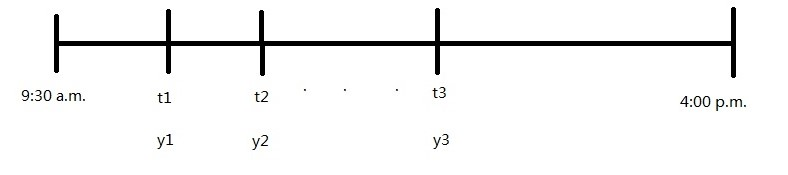
\includegraphics[width=4in]{chapters/chapter_uvts/figures/33d1.jpg}
	\caption{Trading Activities \label{fig:tradeactline}}
	\end{figure}


\section{Trading Decisions as Short-Term Forecast Decisions} 


Most trading decisions generally involve the following considerations
\begin{itemize}
\item How much to trade?
\item When to trade? ie when to enter and when to exit?
\item How to trade? How fast? What is the objective? What are the benchmarks?
\end{itemize}
Answer to these questions involve in some way predicting the market movement and in particular the future (short-term and long-term) price of assets. In the short term it is possible that prices have a tendency to `trend' or exhibit `momentum' but in the long run, prices have a tendency to `mean-revert' as the information about the asset gets incorporated in the price. 


Let $p_{it}$ denote the price of the $i$th asset at time $t$ and let $p_t = (p_{1t},p_{2t},\ldots,p_{nt})$ denote the price vector for `$n$' assets. Let $y_{it}$ denote a vector of characteristics, e.g. volume of transactions, price volatility, number of transactions and the intensity of trading as captured by the average duration between transactions, etc of the $i$th asset at time $t$. These quantities are aggregated from high-frequency data of type given in Table~\ref{tab:CISCO} and illustrated in Figure~\ref{fig:tradeactline} to be used as the characteristics associated with the price changes. In addition, we can also consider factors $f_t = (f_{1t},f_{2t},\ldots,f_{nt})$ that may include market and industry factors as well as asset characteristics such as market capitalization, book-to-market ratio etc. The trading rules can be broadly grouped as follows:
\begin{itemize}
\item[A.] Statistical Arbitrage Rules: $E(p_{i,t+1}\,|\,p_{i,t},p_{i,t-1},\ldots,y_{i,t},y_{i,t-1},\ldots)$
\begin{itemize}
\item[$\bullet$] Predicting the price of $i$th stock at t+1 based on the past trading information; this is sometimes labelled as time series momentum.
\end{itemize}
\item[B.] Momentum: $E(p_{t+1}\,|\,p_{t},p_{t-1},\ldots,y_{t},y_{t-1},\ldots)$
\begin{itemize}
\item[$\bullet$] Predicting the cross-sectional momentum of a subset of stocks based on their past trading characteristics. This is not only useful for portfolio formation and rebalancing, also for pairs trading which is based on tracking two stocks simultaneously so that their divergence can be exploited. 
\end{itemize}
\item[C.] Fair Value: $E(p_{t+1}\,|\,p_{t},p_{t-1},\ldots,V_{t},V_{t-1},\ldots,f_t,f_{t-1},\ldots)$
\begin{itemize}
\item[$\bullet$] Predicting the price using all relevant quantities. Many of these factors can be at a more macro level than the time scale considered for the price prediction, but nevertheless could be useful, as explained in Chapter 3.
\end{itemize}
\end{itemize}
\noindent Thus the price (or alternatively, return) and volatility (or squared return) prediction can be formulated as a time series prediction problem and the common tools such as autoregressive and ARCH models can be used. 


Predicting stock market behavior has been studied extensively starting in the early 20th century. Cowles (1933, 1944)~\cite{cow2,cow1} evaluated the performance of the stock market forecasters. Analyzing the performance of several financial services that made some 7500 recommendations on common stocks over a period, January 1, 1925 to July 1, 1952, it was pointed out the record was worse than the performance of average common stock by 1.43\% annually. Thus `buy-and-hold' strategy out-performed the stock picking strategies of those days. In fact, a much harsher assessment is made: ``A review of the various statistical tests, applied to the records for this period, of these 24 forecasters, indicates that the most successful records are little, if any, better than what might be expected to result from pure chance. There is some evidence, on the other hand, to indicate that the least successful records are worse than what could reasonably be attributed to chance.'' Many of these comments are still valid and have stood the test of the time. Yet, we will demonstrate in this book that there are opportunities for statistical arbitrage. The key is to have access to relevant information and use the appropriate techniques to exploit this in a timely manner. 


\section{Time Series Models for Aggregated Data: Modeling the Mean}

In this section we present a broad overview of the time series models for data aggregated over discrete time intervals. 

\subsection{Stochastic Processes: Some Properties} \hfill

Formally, a discrete time series or stochastic process $Y_1, Y_2, \ldots, \, Y_T$ is a sequence of random variables (r.v.'s) defined on a probability space, and possessing a joint probability distribution, with $Y_t$ denoting the r.v. corresponding to the value of the series at time $t$. A particular sequence of observations of the stochastic process $\{ Y_t, t=1, \ldots,  \, T\}$ is known as a realization of the process. In the analysis of time series we are interested in aspects of the joint probability distribution of collections of random variables such as $Y_1, Y_2, \ldots, \, Y_T$. For such a collection of r.v.'s, the joint distribution function is defined by
	\begin{equation}\label{eqn:feqnfirst}
	F_{12 \ldots T}\left(y_1, y_2, \ldots,  \, y_T\right)= \text{Pr}[Y_1 \leq y_1, Y_2 \leq y_2, \ldots,  	\, Y_T \leq y_T]
	\end{equation}
In general, time series analysis is concerned with determining the properties and identifying the probability structure which generated the observed time series. A general feature of the approach to this analysis is that we do not attempt to study the joint distribution of $Y_1, Y_2, \ldots, \, Y_T$ directly, since this may be too complicated for large $T$, but we study and attempt to describe the probabilistic mechanism which generates the process sequentially through time, and from this to derive the conditional distribution of future observations for purposes of prediction.


Because the means, variances, and covariances are useful summary descriptions of the joint probability distribution of the stochastic process $\{ Y_t, t=1, \ldots,  \, T\}$, we will first consider these quantities. Thus, for any stochastic process $\{Y_t\}$, we define the following functions of $t$:
	\begin{equation}\label{eqn:texteqn}
	\begin{split}
	\text{mean, }\mu(t)&=E(Y_t) \\
	\text{variance, }\sigma^2(t)&=\Var(Y_t)=E[(Y_t-\mu(t))^2] \\
	\text{autocovariance, }\gamma(t,s)&=\Cov(Y_t,Y_s)=E[(Y_t-\mu(t))(Y_s-\mu(s))] \\
	\text{autocorrelation, }\rho(t,s)&=\Corr(Y_t,Y_s)=\dfrac{\gamma(t,s)}{\sigma(t)\sigma(s)}
	\end{split}
	\end{equation}
 Obviously, it is not possible to estimate the many unknown parameters (means, variances, and covariances) under such a general specification from a single realization of $T$ observations. In addition, such generality in the specification of the mean and covariance structure offers no information concerning the prediction of future observations of the process. Hence we must impose some additional structure on the joint distribution of the process in order to substantially reduce the number of unknown parameters, as well as to enable meaningful predictions into the future to be possible. The concept of stationarity of a process is useful in this regard and also serves as a realistic assumption for many types of time series. Stationarity is motivated by the fact that for many time series in practice, segments of the series at different points in time behave similarly, or exhibit homogeneous behavior over time. \\


\noindent \textbf{Stationarity} \\


A time series $\{Y_t\}$ is said to be stationary if for every integer $m$ and any finite set of $m$ time points $t_1, t_2, \ldots, \, t_m$ the set of variables $Y_{t_1}, Y_{t_2}, \ldots, \, Y_{t_m}$ must depend only on the distance between the times $t_1, t_2, \ldots, \, t_m$, rather than on their actual values.  So a stationary process $\{Y_t\}$ tends to behave in a homogeneous manner as it moves through time. The means and variances of the $Y_t$ are the same for all $t$, that is, $E\left(Y_t\right) = \mu$ and  Var$\left(Y_t\right)=\sigma^2$ are constant, for all $t$. So we may express the autocovariance function as 
	\begin{equation}\label{eqn:2gammas}
	\gamma(s)=\Cov(Y_t,Y_{t+s})=E[(Y_t-\mu)(Y_{t+s}-\mu)], \text{ for all }s=0,\pm 1,\cdots
	\end{equation}
Note that by this notation, $\gamma(0) = E[(Y_t-\mu)^2] = \text{Var}(Y_t)$. Also, the \textit{autocorrelation function} of the stationary process may be expressed
        	\begin{equation}\label{eqn:2rhos}
	\rho(s)=\Corr(Y_t,Y_{t+s})= \dfrac{\Cov(Y_t,Y_{t+s})}{\big(\Cov(Y_t)\Cov(Y_t)\big)^{1/2}} = \dfrac{\gamma(s)}{\gamma(0)},  s=0,\pm 1,\cdots
	\end{equation}
$\rho(s)$ will be referred to as the autocorrelation of the process at lag $s$. As we will find, the autocorrelation function (which we will abbreviate as ACF) $\rho(s) = \gamma(s)/\gamma(0)$ of a stationary process $\{Y_t\}$ is a very important tool in describing the characteristics of the process, since it is a convenient summary of the correlation structure of the process over all time lags.  \\


\noindent \textbf{Examples of Stationary Stochastic Processes} 


\begin{ex}[White Noise] \label{ex:whitenoise} Let $\ldots, \epsilon_{-1}, \epsilon_0, \epsilon_1, \ldots$ be a sequence of independent random variables defined on the discrete time points $\ldots,-1,0,1,\ldots$, with mean $E(\epsilon_{t})=0$ and variance $E(\epsilon_{t}^2)=\sigma^2$, for all $t$. Set $Y_t = \mu + \epsilon_t, \, t=0, \pm1, \ldots$. Then $E(Y_t)=\mu$ for all $t$, and since independence implies that the random variables are uncorrelated, we have $\Cov(Y_t,Y_{t+s})=\Var(Y_t)=\sigma^2$ if $s=0$ and $\Cov(Y_t,Y_{t+s})=0$ if $s\neq0$. Thus the process is stationary. Such a process is referred to as purely random process or a \textit{white noise process}, and will be found to be the foundation for the construction of many other processes of interest. 
\end{ex}


\begin{ex}[Moving Average] \label{ex:movingaverage} Let $\{\epsilon_t\}$ be independent r.v.'s as in Example~\ref{ex:whitenoise}, and define a new process $\{Y_t\}$ by
	\[
	Y_t = \mu + \epsilon_t + \epsilon_{t-1}, \qquad t=0, \pm1, \cdots
	\]
where $\mu$ is a constant.  Then $E(Y_t)=\mu$, for all $t$, and
	\[
	\Cov(Y_t,Y_{t+s})=\gamma(s)=
	\begin{cases}
	 2\sigma^2 & \text{if } s=0 \\
	  \sigma^2 & \text{if } s=1 \\
	  0 & \text{if } s>1 \\
	\end{cases}
	\]
which depends only on the time lag $s$ and not on $t$.  Hence the process $\{Y_t\}$ is stationary with ACF $\rho(s)=\gamma(s)/\gamma(0)$ such that $\rho(0)=1$, $\rho(1)=1/2$ and $\rho(s)=0$ for $|s|>1$.
 
            \begin{sidewaysfigure}[hbp] %htbp
                %\centering
                \label{chap2fig2}
                \subfigure[Figure 1a]
                        [Time series plot of $0.5 + \epsilon_t$]
                        {
                        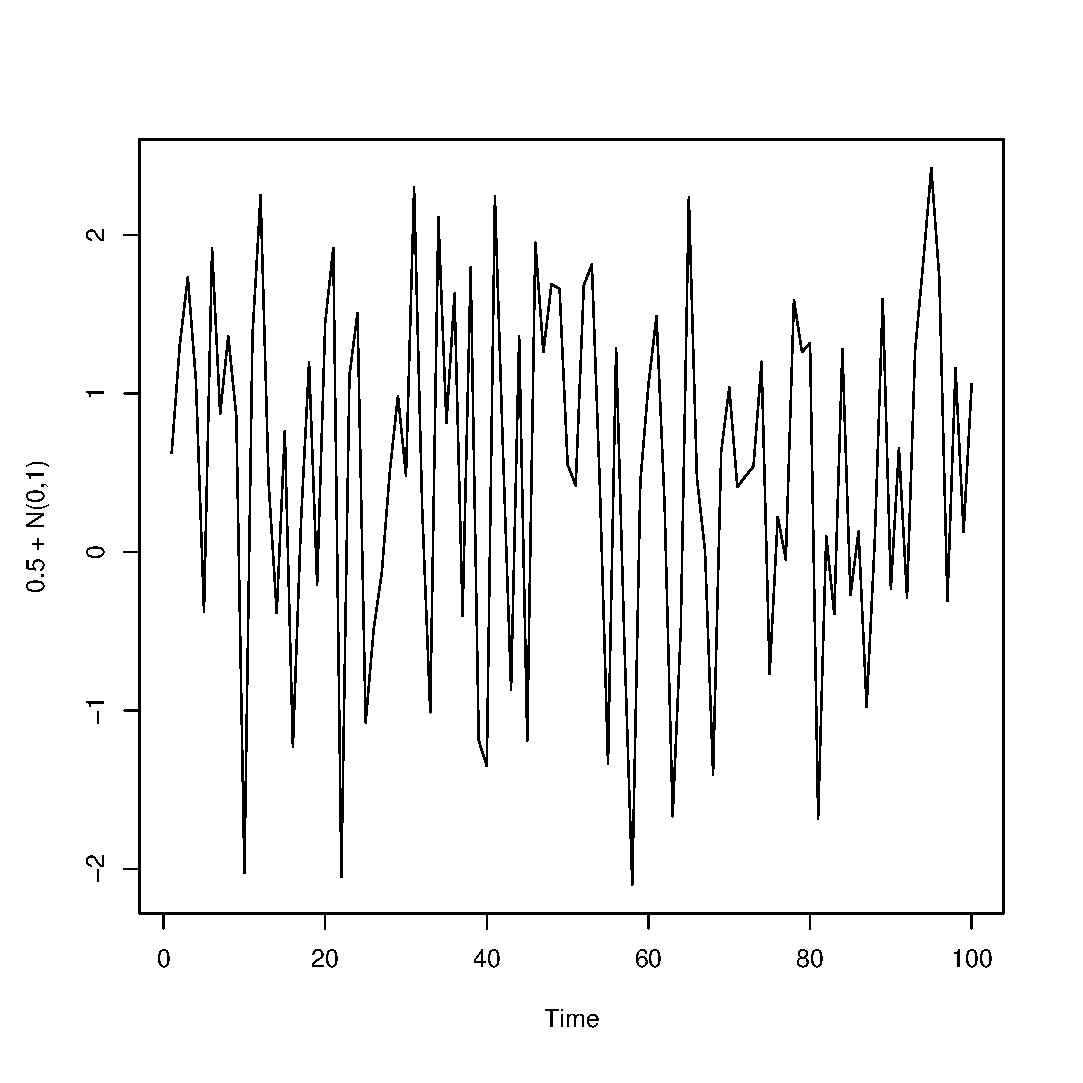
\includegraphics[scale=0.32]{chapters/chapter_uvts/figures/ch1fig1y1ts.eps}
                        }
                        \hfill
                \subfigure[Figure 1b]
                        [ACF]
                        {
                        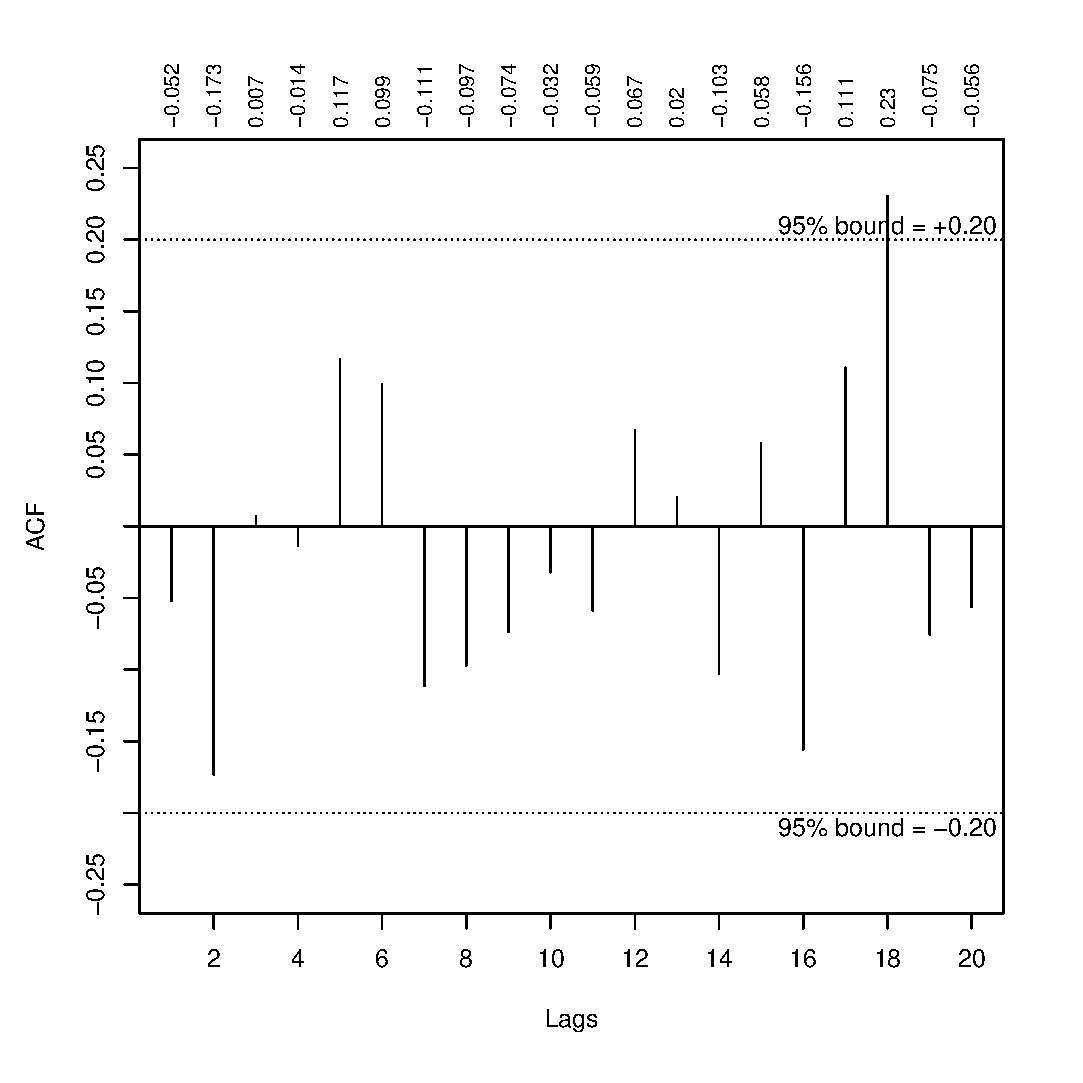
\includegraphics[scale=0.32]{chapters/chapter_uvts/figures/ch1fig1y1acf.eps}

                        }
                        \hfill
                %\subfloat[Figure 1ab][Time Series Plot \& ACF Plot]
                %{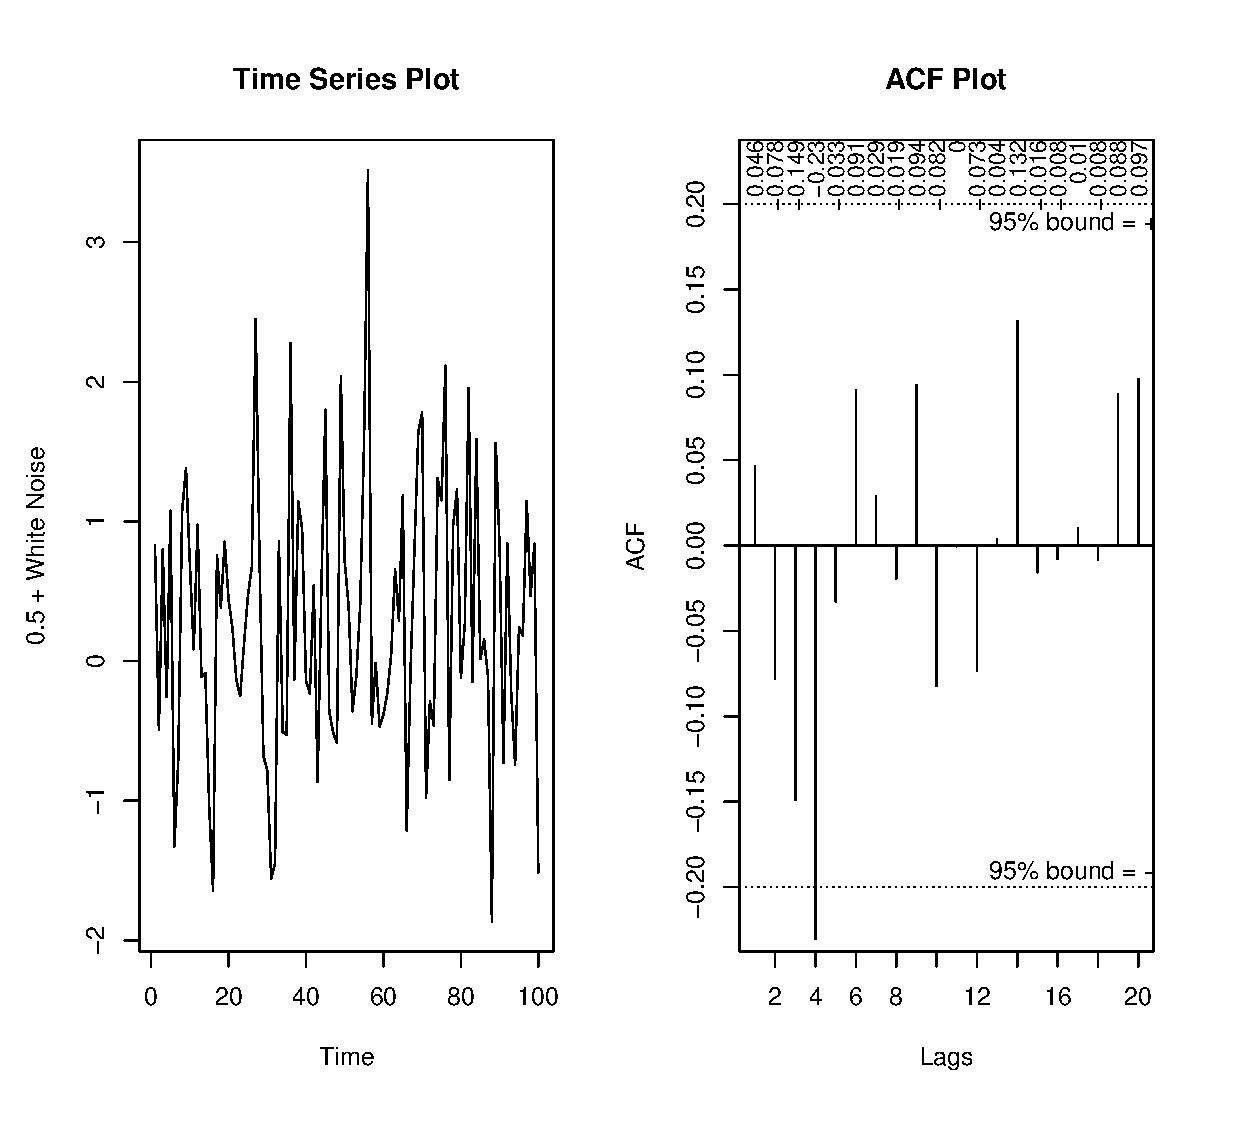
\includegraphics[width=\textwidth, height=0.5\textheight]{ch1fig1y1ab.eps}}
                %\qquad
                \subfigure[Figure 1c]
                        [$Y_t$ vs. $Y_{t-1}$]
                        {
                        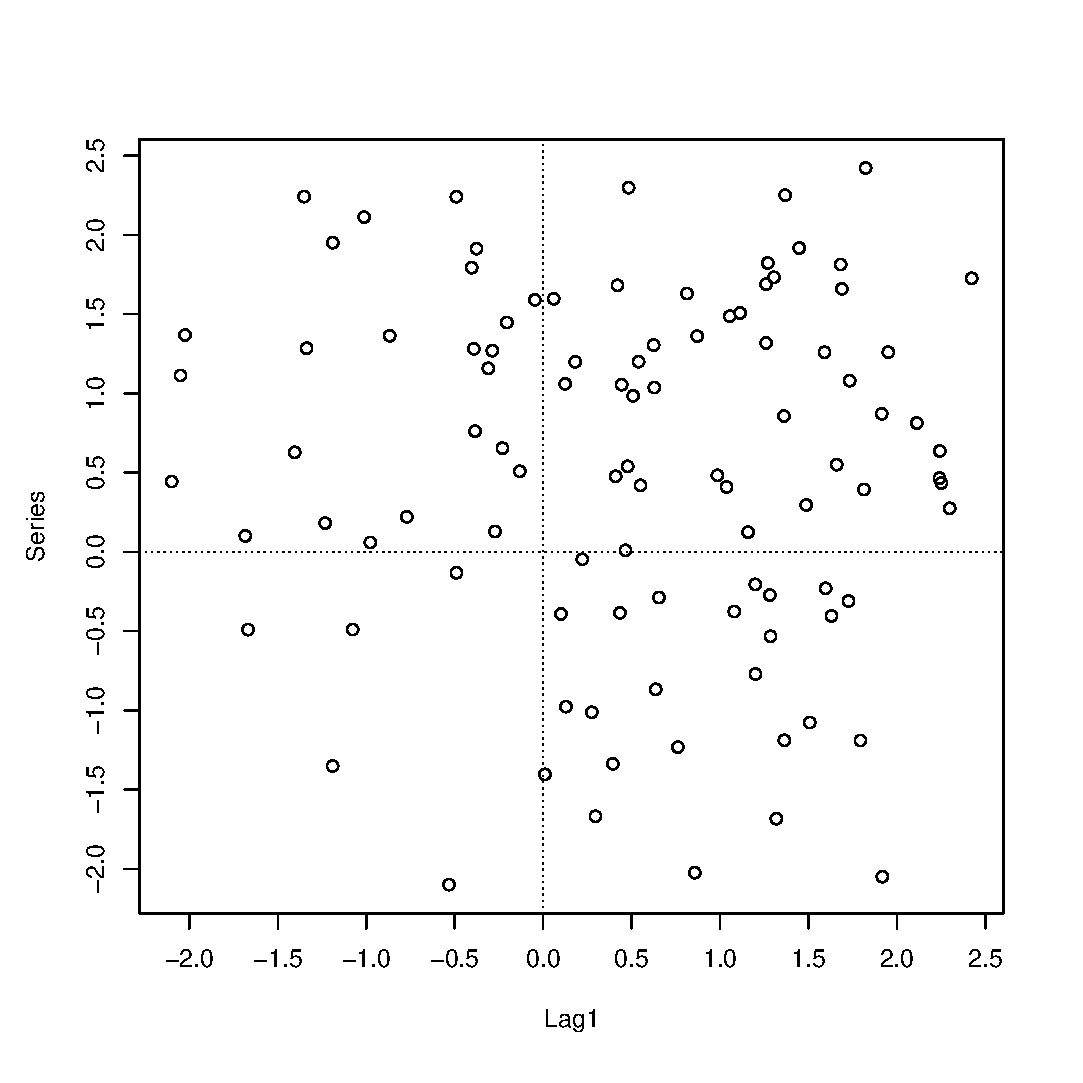
\includegraphics[scale=0.32]{chapters/chapter_uvts/figures/ch1fig1y1lagplot.eps}

                        }
                %%%%%%
                \quad           %\qquad
                %%%%%
                \subfigure[Figure 1d]
                        [Time series plot of $1.0 + \epsilon_t + \epsilon_{t-1}$]
                        {
                        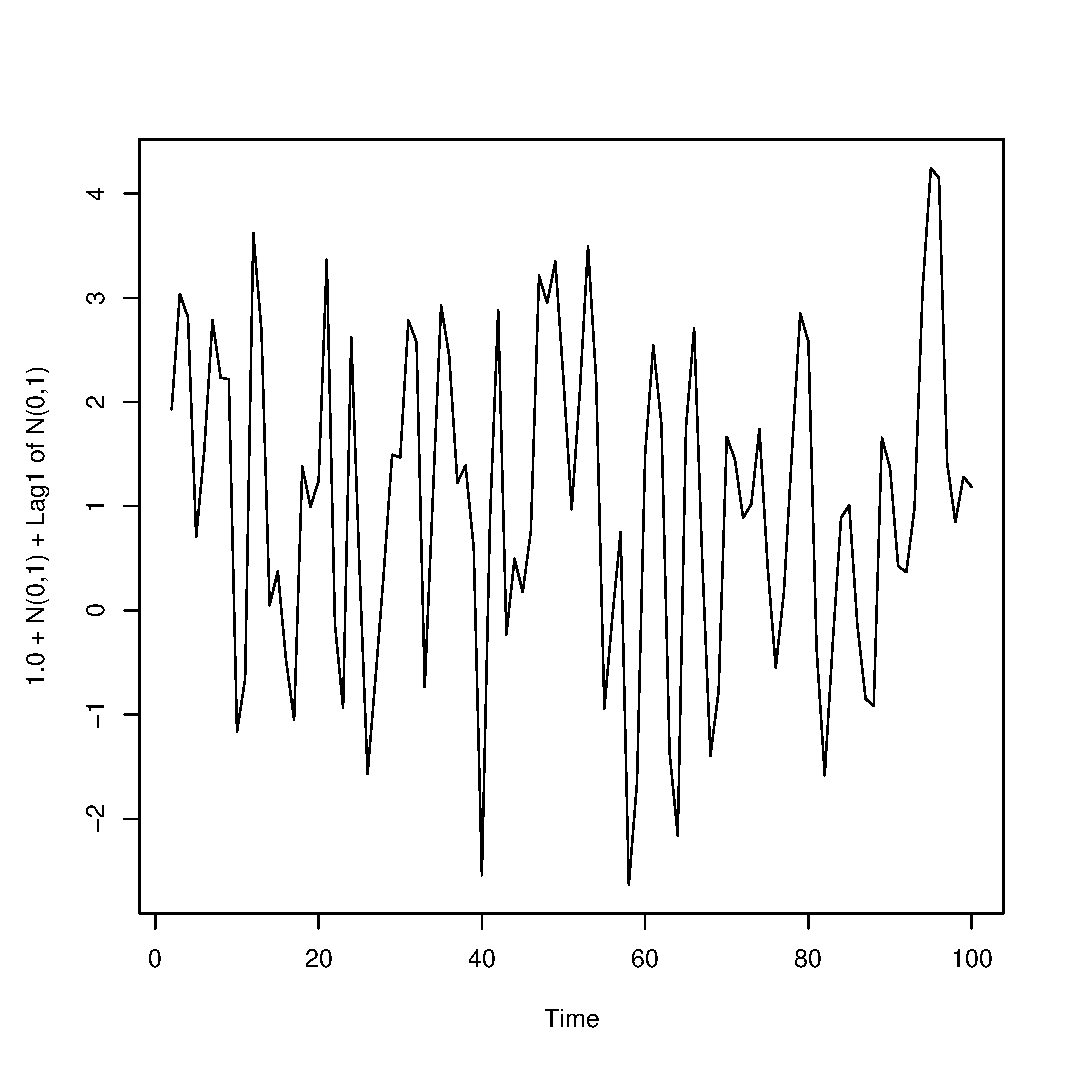
\includegraphics[scale=0.32]{chapters/chapter_uvts/figures/ch1fig1y2ts.eps}

                        }
                        \hfill
                \subfigure[Figure 1e]
                        [ACF]
                        {
                        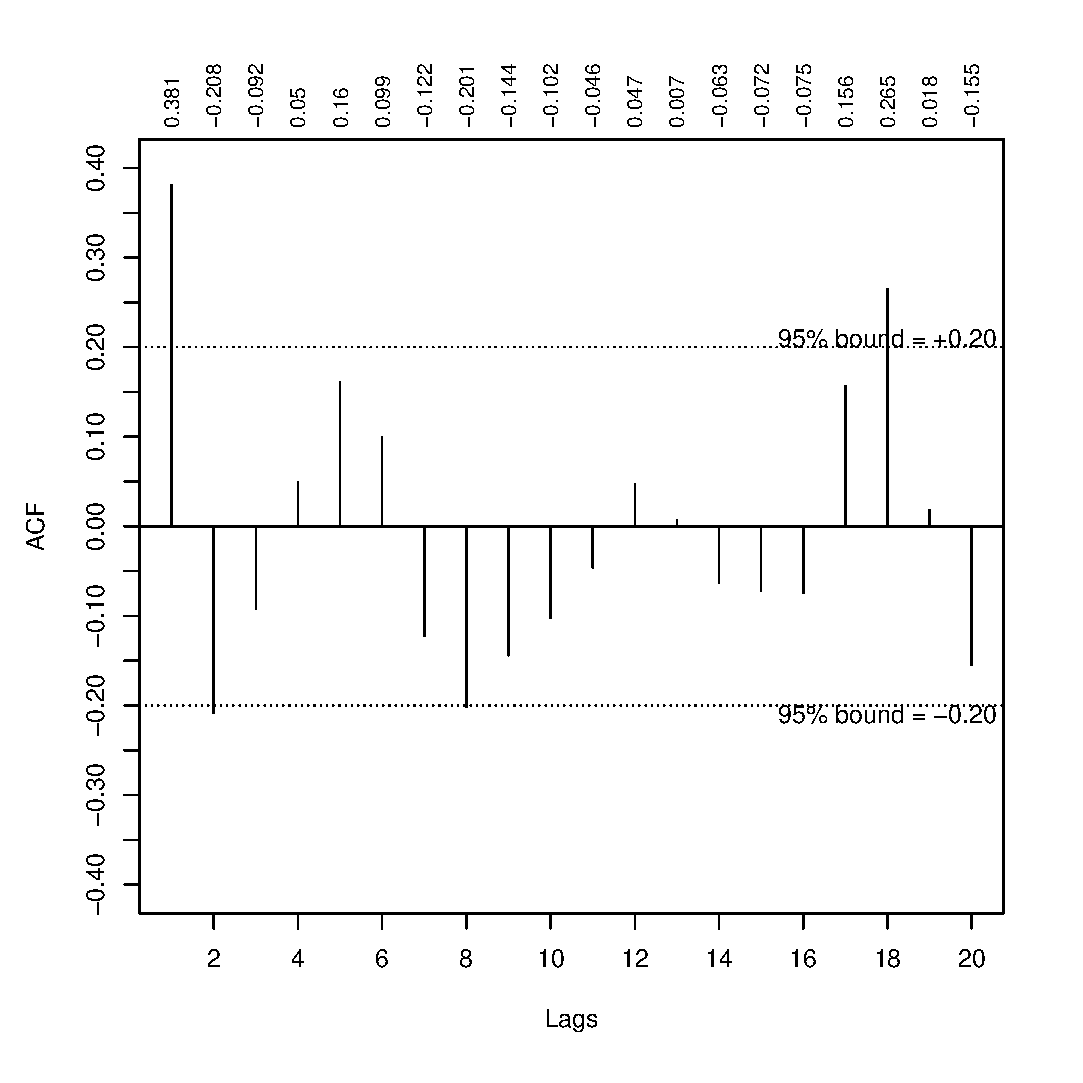
\includegraphics[scale=0.32]{chapters/chapter_uvts/figures/ch1fig1y2acf.eps}

                        }
                        \hfill
                \subfigure[Figure 1f]
                        [$Y_t$ vs. $Y_{t-1}$]
                        {
                        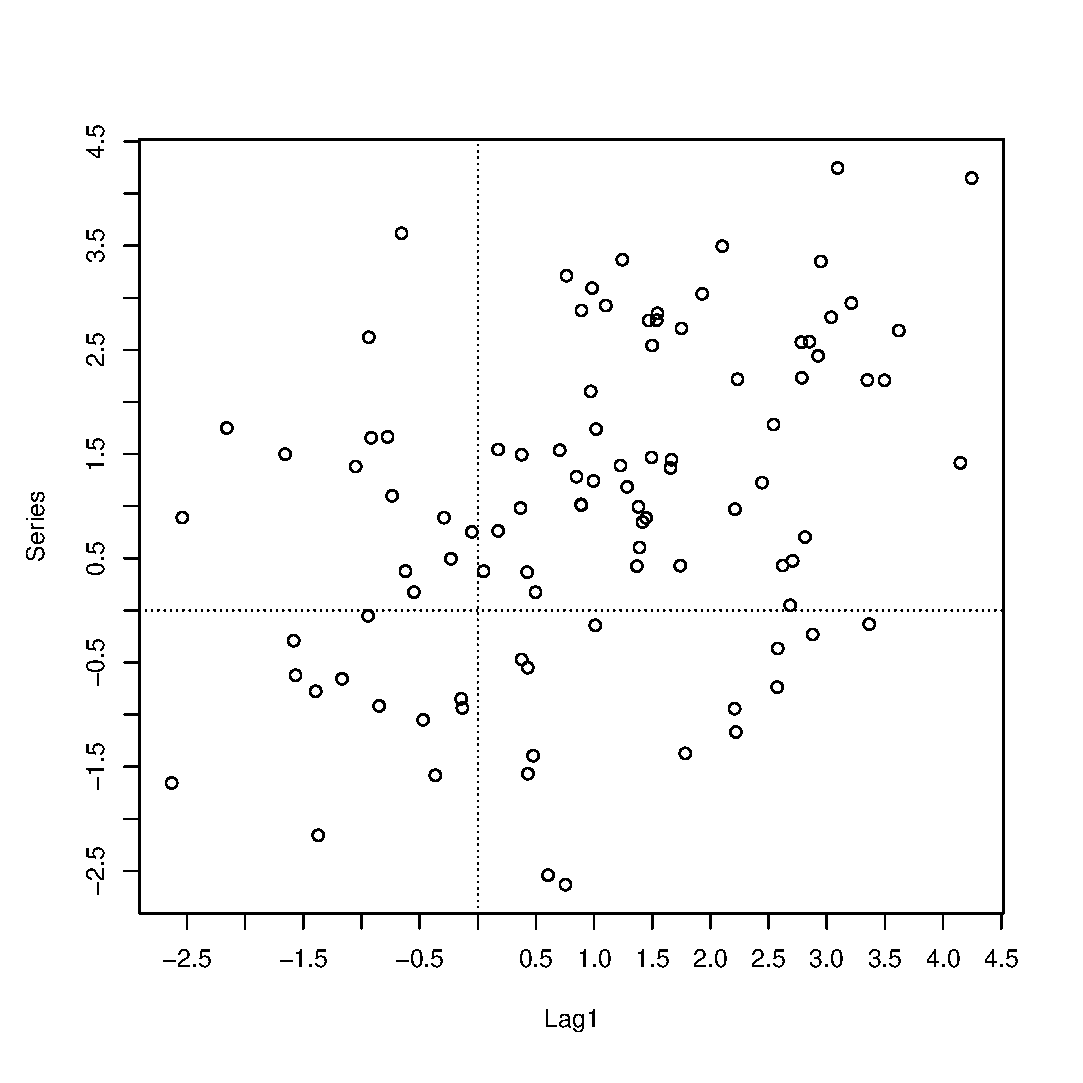
\includegraphics[scale=0.32]{chapters/chapter_uvts/figures/ch1fig1y2lagplot.eps}

                        }
               \caption{Processes \& Diagnostics from $Y_t = 0.5 + \epsilon_t$ and from $Y_t =1.0 + \epsilon_t + \epsilon_{t-1}$\label{fig:sideways}}
            \end{sidewaysfigure}


Figure~\ref{fig:sideways}~(a) shows a time series plot of a computer simulated series of 100 values from a Gaussian white noise process $\{\epsilon_t\}$ with $\sigma^2=1$, while Figure~\ref{fig:sideways}~(b) shows a plot of the corresponding values of the series $Y_t = 1.0 + \epsilon_{t} + \epsilon_{t-1}$ using these same $\{\epsilon_t\}$.  Note the relatively much smoother behavior over time of the data in (b) than in (a), due to the positive autocorrelation at lag one of the process in (b) which tends to make successive values of the series behave more similarly to each other.  Similar to the last example, it is easy to show that the process $\{Y_t\}$ defined by the relation $Y_t = \mu + \epsilon_{t} - \epsilon_{t-1}$ is stationary with autocorrelation function $\rho(0)=1$, $\rho(1)=-1/2$, and $\rho(s)=0$ for $|s|>1$. A plot of a simulated series from this process is given in Figure~\ref{fig:sideways}~(d) where the much ``rougher'' or less smooth behavior over time relative to the behavior  in (a) and (b) due to the addition of extra noise to the model. These figures form the basis of model building and the subsequent diagnostic checks on the fitness of models. 
\end{ex} 


\noindent \textbf{Examples of Nonstationary Stochastic Processes} \\


Many time series that occur in finance do not exhibit stationary behavior.  For example, many stock price series show a trend or change in the mean level over time, reflecting information flow about the stock or investors' behavior. Series also exhibit seasonal behavior, either in the form of nonstationary or deterministic seasonal patterns, both of which need to be distinguished from purely nondeterministic stationary stochastic behavior. Other departures from stationarity include changes in variability of the process over time (nonconstant variance or volatility regimes), abrupt shifts in the mean level, and changes in the autocorrelation structure of the process over time which is a feature of the series which would typically be more difficult to detect.  An important practical matter in the analysis of time series data involves methods of transforming a possibly nonstationary time series into a stationary series, and accounting for and modeling of the nonstationary aspects of the original series.  Many of the methods that are found useful in practice involve considering successive changes or differences over time in the original series to remove the nonstationary features of the series, especially changes in the mean level, or using linear regression techniques to help account for the nonstationary mean behavior.  We will illustrate this with a few simple examples. 


\begin{ex}[Random Walk with a Drift] \label{ex:driftwalk} Let $\{\epsilon_t, \, t=0,1,2, \ldots\}$ be a sequence of independent random variables with mean 0 and variance $\sigma^2$, and define a new process $\{Y_t\}$ recursively by
	\[
	Y_t = Y_{t-1} + \delta + \epsilon_t, \qquad t=0,1,2, \ldots, \quad Y_0 = 0,
	\]
where $\delta$ is a constant.  By successive substitutions in the above relations for $Y_t$, we find that $\{Y_t\}$ can also be expressed as
	\[
	Y_t = \delta \, t + \sum_{j=1}^t \epsilon_j= \delta \, t + \epsilon_{t} + \epsilon_{t-1} + \ldots + \epsilon_{1}, \qquad t=1,2, \ldots .
	\]
Hence we see that $E(Y_t)=\delta t$ and $\Var(Y_t)= \Var(\sum_{j=1}^t \epsilon_j)= \sum_{j=1}^t\Var(\epsilon_j)=t \, \sigma^2$, so that the process $\{Y_t\}$ is not stationary and exhibits change in both mean and variance.  Moreover, for any $s>0$, we find that
	\[
	\Cov(Y_t,Y_{t+s})= \Cov\left(\sum_{j=1}^t \epsilon_j, \sum_{i=1}^{t+s} \epsilon_i\right)= \sum_{j=1}^t\text{Var}(\epsilon_j)= t \, \sigma^2 \, ,
	\]
so that $\Corr(Y_t,Y_{t+s}) = t / \sqrt{t(t+s)} = 1/ \sqrt{1+s/t}$. Note that this correlation is close to one for large $t$ and relatively small $s$, so that nearby values $Y_t$ and $Y_{t+s}$ of the process $\{Y_t\}$ are highly positively correlated.  However, note that the time series of successive changes or \textit{first differences} of the process $\{Y_t\}$, defined by $Z_{t}=Y_{t}-Y_{t-1}$, does form a stationary process, since $Z_{t}=Y_{t}-Y_{t-1} = \delta + \epsilon_t$, a white noise series as in Example~\ref{ex:whitenoise}. Such a process $\{Y_t\}$ whose first differences form a white noise series, is called a random walk process. Time series plots of simulated data from random walk exhibit behavior with little tendency to vary around a fixed constant mean level. The parameter $\delta$ in the random walk model is referred to as the drift in the random walk process. Note the trend behavior in the process with $\delta>0$.
\end{ex}


Of course, a more general class of models is obtained by supposing that a nonstationary process $\{Y_t\}$ is such that its first differences form a stationary process, but not necessarily white noise.  It has been found from practical experience that this type of model is quite useful in producing adequate representations for actual observed financial series in many cases.


\subsection{Some Basic Models and Descriptive Tools} \hfill


Suppose we have a sample realization of $T$ observations $Y_1, Y_2, \ldots, Y_T$ from a stationary process $\{Y_t\}$ which has a mean $\mu=E(Y_t)$, autocovariance function (ACF) $\gamma(s)=\Cov(Y_t,Y_{t+s})$ and autocorrelation function $\rho(s)=\Corr(Y_t,Y_{t+s}) = \gamma(s)/\gamma(0)$. Since the theoretical ACF $\rho(s)$ is such a basic quantity which describes the correlation properties of the process, we are naturally interested in obtaining estimates of $\rho(s)$ from the sample data.


First, a natural estimator of $\mu$ is the sample mean $\overline{Y}=(1/T)\sum_{t=1}^T Y_t$. The most common estimator used for $\gamma(s)$ is the sample autocovariance function defined by
	\[
	\hat{\gamma}(s)= \frac{1}{T} \sum_{t=1}^{T-s} \, \left(Y_{t}-\overline{Y}\right) \left(Y_{t+s}-\overline{Y}\right), \enskip s=0, 1, \ldots
	\]
Usually one only computes $\hat{\gamma}(s)$ for lags $s$ much smaller than $T$, say, $0 \leq s \leq T/4$, since $\hat{\gamma}(s)$ for large lags are typically not very informative or of much interest. Note that $\hat{\gamma}(s)$ has the form of an ordinary sample covariance between the pairs of variables $(Y_t, Y_{t+s})$, except for the use of the common sample mean $\overline{Y}$ for both variables and the divisor $T$ in place of $T-s$.  Note also that $\hat{\gamma}(0) = T^{-1}\sum_{t=1}^T(Y_t-\overline{Y})^2$ represents the sample variance of the data.  The estimator of $\rho(s)$ follows directly from $\hat{\gamma}(s)$ and is given by
	\begin{equation}\label{eqn:hatrho}
         \hat{\rho}(s) = \frac{\hat{\gamma}(s)}{\hat{\gamma}(0)}= \frac{\sum_{t=1}^{T-s} \, \left(Y_{t}-\overline{Y}\right) \left(Y_{t+s}-\overline{Y}\right)}{\sum_{t=1}^T(Y_t-\overline{Y})^2}\, , \enskip s = 0, 1, \ldots 
	\end{equation}
which is called the sample ACF.  The sample ACF will also sometimes be denoted as $\hat{\rho}(s) \equiv r(s)$.


We now briefly discuss a few properties of the sampling distributions of the above estimators, with particular emphasis on the sample ACF $r(s)$.  The mean of $\overline{Y}$ is easily seen to be $E(\overline{Y})=(1/T)\sum_{t=1}^T E(Y_t) = \mu$, so that $\overline{Y}$ is an unbiased estimator of $\mu$.  The variance of $\overline{Y}$ is
	\begin{equation} \label{eqn:var}
	\begin{split}
        \Var\left(\overline{Y}\right)&= \frac{1}{T^2} \Var\left( \sum_{t=1}^T Y_t\right) \\
                &= \frac{1}{T^2} \left[ \sum_{t=1}^T \text{Var} (Y_t) + 2 \sum_{t=1}^{T-1}\sum_{u=1}^{T-t} \Cov(Y_t, Y_{t+u}) \right] \\
                &= \frac{1}{T^2} \left[ T \gamma(0) + 2 \sum_{t=1}^{T-1}\sum_{u=1}^{T-t} \gamma(u) \right] \\
                 &= \frac{\gamma(0)}{T} \left[1 + 2 \sum_{u=1}^{T-1} \frac{T-u}{T}\rho(u)\right]  
        \end{split}              
        \end{equation}
Hence if $\rho(u) \rightarrow 0$ as $u \rightarrow \infty$, then so that $\Var\left(\overline{Y}\right) \rightarrow 0$ as $T \rightarrow \infty$. This implies that $\overline{Y}$ converges in probability to $\mu$ and from Equation~\ref{eqn:var} $\text{Var}\left(\overline{Y}\right) = \gamma(0)/T$ occurs when $\rho(u)=0$ for all $u \neq 0$; that is, when the $Y_t$ are mutually uncorrelated.  Under some mild conditions it can also be shown that $\overline{Y}$ is asymptotically normally distributed as $T \rightarrow \infty$.


The sampling properties of the sample ACF $r(s)$ are quite complicated and exact results are not available except in a few special cases. We indicate one result from Anderson and Walker (1964)~\cite{anderwalk} based on large sample theory. Under linearity of the time series, the joint distribution of $T^{1/2}(r(1)-\rho(1)),\ldots$,  $T^{1/2}(r(k)-\rho(k))$, $k$ fixed, tends to a multivariate normal $N(0, W)$ distribution as $T \rightarrow \infty$ where $W$ is a $k \times k$ matrix with $(i,j)$th element $w_{ij}$ given by
	\begin{equation} \label{eqn:wij}
	\begin{split}
            w_{ij}= \sum_{\nu= -\infty}^\infty \,& [\, \rho(\nu+i)\rho(\nu+j) + \rho(\nu-i)\rho(\nu+j) - 2 \rho(\nu)\rho(j)\rho(\nu+i)  \\
                     &- 2 \rho(\nu)\rho(i)\rho(\nu+j) + 2 \rho(\nu)^2 \rho(i)\rho(j) \, ],  i, j= 1,\ldots, k. ]
        \end{split}
	\end{equation}
Hence for large $T$ we have the approximations $E(r(s)) \approx \rho(s)$, $\Var(r(s)) \approx w_{ss}/T$, $\Cov(r(s), r(u)) \approx w_{su}/T$, and the $r(s)$ are approximately normally distributed. The Equation~\ref{eqn:wij} is also called Bartlett's formula and dates back to 1946.


There are a few special cases of Equation~\ref{eqn:wij} worth noting. In the purely random or white noise case where the $Y_t$ are independent r.v.'s, we then have $\rho(\nu)=0$ for all $\nu \neq 0$ and so the approximations reduce to $E(r(s)) \approx 0$, $\Var(r(s)) \approx 1/T$, $\Cov(r(s), r(u)) \approx 0$, or more exactly, $\Var(r(s)) \approx (T-s)/T^2$. Hence we can use these results to check for ``non-randomness'' of a series of comparing the sample values $r(s)$ at various lags $s=1, \ldots, k$ with the approximate 95\% limits $\pm \, 2 \sqrt{(T-s)/T^2} \approx 2 / \sqrt{T}$ for the normal distribution to see whether the $r(s)$ generally fall within these limits. We will use this test repeatedly as a diagnostic tool for model adequacy. 


For a second case, suppose it is assumed that the theoretical ACF satisfies $\rho(\nu) = 0$ for all $|\nu| > q$.  Then, for any $s>q$ the expression for the approximate variance of $r(s)$ reduces to
	\begin{equation}\label{eqn:varrs}
	\Var(r(s)) \approx \dfrac{1}{T} \sum_{\nu=-q}^q \rho(\nu)^2= \dfrac{1}{T} \left[ 1+ 2 \sum_{\nu=1}^q \rho(\nu)^2 \right], \enskip s>q 
	\end{equation}        
and
	\[
	\Cov(r(s), r(u))\approx \frac{1}{T} \sum_{\nu = -q}^{q} \, \rho(\nu) \rho(\nu -s+u),\enskip s, u > q.
	 \]

As one final special case, suppose the process  has ACF of the simple form (which results from an autoregressive model of order one (AR(1)), defined later) $\rho(\nu) = \phi^{|\nu|}$, $\nu=0, \pm 1, \ldots$, with $|\phi| < 1$. Then
	\[
	\Var(r(s)) \approx \frac{1}{T} \left[\frac{(1+\phi^2)(1-\phi^{2s})}{1-\phi^2} - 2s\phi^{2s}\right],
	\]
and in particular $\text{Var}(r(1)) \approx \frac{1}{T} (1-\phi^2)$.


The plot of ACF for a white noise sequence for a large number of lags may have a few isolated lags lie outside the limits, $\pm \frac{2}{\sqrt{T}}$. But characteristic behavior of nonstationary series is that the sample ACF values $r(s)$ are slow to ``dampen out'' as the lag $s$ increases. \\


\noindent\textbf{Linear Models for Stationary Time Series} \\


A stochastic process $\{Y_t\}$ will be called a \textit{linear process} if it can be represented as the output of a (one-sided) absolutely summable linear filter with white noise input process $\{\epsilon_t\}$; that is,
	\begin{equation}\label{eqn:yt}
          Y_t = \mu + \sum_{j=0}^{\infty}  \psi_j \,  \epsilon_{t-j}
	\end{equation}
where the $\epsilon_t$ are independent with 0 mean and variance $\sigma^2_{\epsilon}$, and $\sum_{j=0}^{-\infty} \, |\psi_j | < \infty$. This process may also be referred to as an infinite moving average process.


We now introduce, for notational convenience, the backward shift operator $B$, defined by the property that $B\,Y_t = Y_{t-1}$ for any time series $\{Y_t\}$. Hence, on successive applications, we obtain $B^j \, Y_t = Y_{t-j}$ and the infinite moving average (\ref{eqn:yt}) may be expressed as
	\[
	Y_t = \mu + \sum_{j=0}^{\infty} \psi_j \,  B^j \, \epsilon_t = \mu + \psi(B) \, \epsilon_t,
	\]
where $\psi(B) = \psi_0 + \psi_1 \, B + \psi_2 \, B^2 + \cdots$ is referred to as the infinite moving average operator. Since the input $\{\epsilon_t\}$ is a stationary process, it follows that $\{Y_t\}$ in (\ref{eqn:yt}) forms a stationary process, with mean $E(Y_t)=\mu$ and autocovariance function
	\begin{equation}\label{eqn:covyt}
	\begin{split}
	\gamma(s)= \Cov(Y_t, Y_{t+s})&=E \left[ \sum_{j=0}^{\infty} \, \sum_{k=0}^{\infty} \psi_j \, \psi_k \, \epsilon_{t-j} \, \epsilon_{t+s-k} \right] \\
	&=\sum_{j=0}^{\infty} \, \sum_{k=0}^{\infty} \psi_j \, \psi_k \, \gamma_{\epsilon}(j-k+s) \\
	&=\sigma^2_{\epsilon} \, \sum_{j=0}^{\infty} \psi_j \, \psi_{j+s},
	\end{split}
	\end{equation}      
since $\gamma_{\epsilon}(s) = \sigma^2_{\epsilon}$ if $s=0$ and $\gamma_{\epsilon}(s) = 0$ if $s \neq 0$, so that $\gamma_{\epsilon}(j-k+s) = 0$ when $k \neq j=s$.
	

The following theorem indicates the generality of the class of linear processes in stationary theory, in the sense that every purely non-deterministic stationary process may be expressed in an infinite moving average representation as in (\ref{eqn:yt}), although the $\epsilon_t$ need not be independent but merely uncorrelated.	


\begin{thm}[Wold's Theorem] \label{thm:wold}
Let $Y_t, t=0, \pm 1, \ldots$, be a purely non-deterministic weakly stationary stochastic process with mean $\mu$. Then $Y_t$ may be expressed as
	\[
	Y_t = \mu + \sum_{j=0}^{\infty} \psi_j \, \epsilon_{t-j},
	\]
with  $\psi_0 = 1$, $\sum_{j=0}^{\infty} \psi_j^2 < \infty$ where the $\epsilon_t$ are uncorrelated random variables with $E(\epsilon_t)=0$ and $\text{Var}(\epsilon_t)=\sigma^2_{\epsilon}$ for all $t$. The r.v. $\epsilon_t$ is called the innovation or random shock at time $t$.
\end{thm}


The general linear representation model given by (\ref{eqn:yt}) although useful for studying the properties of time series models but is not directly useful in practice to represent a stationary process, since it requires the determination of an infinite number of unknown parameters $\psi_1,\psi_2, \ldots$, from a finite record of data. Hence we now consider finite parameter models of the same type which will be useful representations. These models essentially express the infinite number of coefficients $\psi_j$ in terms of a finite number of parameters, and the particular classes of finite parameter models considered are sufficiently general to well approximate the model for any process of the form (\ref{eqn:yt}). \\


\noindent \textbf{Finite Moving Average Processes} \\


A direct way to obtain finite parameter models from the general form (\ref{eqn:yt}) is simply to restrict the $\psi_j$ to be zero beyond some lag $q$. Thus (with a change of notation), a stationary process $\{Y_t\}$ is said to be a \textit{moving average process} of order $q$, which is denoted as MA($q$), if it satisfies
	\begin{equation}\label{eqn:yt2}
	Y_t = \mu + \epsilon_t - \sum_{j=1}^{q} \theta_j \epsilon_{t-j},
	\end{equation}
where the $\epsilon_t$ are independent with mean 0 and variance $\sigma^2$. Using the backward shift operator notation $B$, the MA($q$) model can be expressed as
	\begin{equation*}
	\begin{split}
         Y_t & = \mu + \epsilon_t - \sum_{j=1}^q \theta_j \, B^j \, \epsilon_t \\
                & = \mu + (1 - \theta_1 \, B - \theta_2 B^2  - \cdots - \theta_q \, B^q) \epsilon_t= \mu + \theta(B) \, \epsilon_t,	
	\end{split}
	\end{equation*}
where $\theta(B) = 1 - \sum_{j=1}^q \theta_j \, B^j$.  An MA($q$)  process is always stationary, by Theorem~\ref{thm:wold}, since $\sum_{j=0}^{\infty} |\psi_j|= 1 + \sum_{j=1}^q |\theta_j|$ is always finite. The mean of the process is $\mu = E(Y_t)$, and the autocovariance function is (from (\ref{eqn:covyt}))
	\begin{equation*}
	\begin{split}
            \gamma(s) = \text{Cov}(Y_t, Y_{t+s})&= \sigma^2 (-\theta_s + \theta_1 \, \theta_{s+1} + \cdots + \theta_{q-s} \, \theta_q ) \\
                &= \sigma^2 \sum_{j=0}^{q-s} \theta_j \, \theta_{j+s}, \enskip s = 0, 1, 2, \ldots, q,	
	\end{split}
	\end{equation*}
and $\gamma(s)=0$ for $s>q$, where $\theta_0$ is defined to be $-1$. So in particular, $\gamma(0)= \Var(Y_t) = \sigma^2 (1 + \sum_{j=1}^q \theta_j^2)$. Hence the autocorrelation function of an MA($q$) process (\ref{eqn:yt2}) is
       \begin{equation}\label{eqn:rhos}
	\rho(s) = \dfrac{-\theta_s + \sum_{j=1}^{q-s} \theta_j \, \theta_{j+s}}{1 + \sum_{j=1}^q \theta_j^2}, \enskip s = 0,1,\ldots, q
       \end{equation}
and $\rho(s)=0$ for $s>q$. The prominent feature of the ACF of an MA($q$) process is that it equals zero or ``cuts off'' after a finite number of lags, $q$. Thus in one sense the ``memory'' of an MA($q$) process is $q$ periods long. In practice, useful MA($q$) models are those for which the value of $q$ is typically quite small, such as $q=1,2,$ or $3$.  For financial time series, usually $q=1$ will suffice for modeling, which we will discuss below. 


\begin{ex}[Moving Average Model of Order 1]\label{ex:movingorder1}
The simplest example of a moving average process is that of order one, MA(1), given by
	\[
	Y_t = \mu + \epsilon_t - \theta \epsilon_{t-1}= \mu + (1 - \theta B) \epsilon_t.
	 \]
Its autocovariances are $\gamma(0)= \sigma^2(1+\theta^2)$, $\gamma(1)= -\theta \sigma^2$, and $\gamma(s)=0$ for $s>1$, and hence the ACF is $\rho(1)= -\theta /(1+\theta^2)$, $\rho(s)=0$, $s>1$. It is easy to show that the largest possible value of $\lvert\rho(1)\rvert= \lvert\theta\rvert / (1+\theta^2)$ for an  MA(1) process is $\rho(1)=\pm 0.5$ which occurs when $\theta = \pm 1$. This illustrates that in general there are further restrictions on the autocorrelation function $\rho(s)$ of an MA($q$)  process in addition to $\rho(s)=0$, $s>q$. These restrictions are essentially the result of the requirement that the autocorrelation function $\rho(s)$ of the MA($q$) process be positive semidefinite.
\end{ex}
    

\begin{ex}[Seasonal Moving Average]\label{ex:seasonal} 
For time series which may exhibit seasonal correlation, such as certain financial time series with week-day effect, the following type of special seasonal MA model is useful. Let $S$ denote the number of discrete time periods per seasonal period (for example, $S=4$ for quarterly data of an annual seasonal nature), and define the process $\{W_t\}$ by
	\[	
	W_t = \mu + \epsilon_t - \tau_S \, \epsilon_{t-S}
	\]
Then we find that $\gamma(0)= \sigma^2(1+\tau_S^2)$, $\gamma(S) = - \tau_S / (1+\tau_S^2)$,  and $\rho(j)=0$ for all $j \neq 0, \pm S$. Hence this process exhibits nonzero autocorrelation only at the seasonal lag $S$. This model is known as a seasonal MA model of seasonal order 1 (and period $S$), and its generalizations are useful when modeling seasonal differences $W_t = Y_t - Y_{t-S}$ of an original seasonal time series $\{Y_t\}$.  In the context of financial data, this could be used to model the so called Monday and Friday effects.
\end{ex}      


\begin{ex}[Autoregressive Model of Order 1]\label{ex:autoregor1}
Consider the process (\ref{eqn:yt}) with coefficients given by $\psi_j = \phi^j$, $j=0,1,\ldots$,  for some $\phi$ with $\lvert\phi\rvert<1$. Then the process $Y_t = \mu + \sum_{j=0}^{\infty} \phi^j \, \epsilon_{t-j}$ is stationary, since $\sum_{j=0}^{\infty} \, \lvert\psi_j\rvert= \sum_{j=0}^{\infty} \, \lvert\phi\rvert^j = 1/(1-\lvert\phi\rvert)$ is absolutely convergent for $\lvert\phi\rvert < 1$. From (\ref{eqn:covyt}), the autocovariance function of $\{Y_t\}$ is
	\[
	\gamma(s)= \sigma^2_{\epsilon} \sum_{j=0}^{\infty} \phi^j \, \phi^{j+s}= \sigma^2_{\epsilon} \, \phi^s \sum_{j=0}^{\infty} \phi^{2j}= \frac{\sigma^2_{\epsilon} \, \phi^s}{1 - \phi^2}, \enskip s \geq 0.
	\]
In particular, $\gamma(0) = \Var(Y_t) = \sigma^2_{\epsilon}/(1-\phi^2)$. Hence the autocorrelation function of $\{Y_t\}$ is $\rho(s)= \gamma(s)/\gamma(0)= \phi^s$, $ s \geq 0$ which declines exponentially (geometrically) as the lag $s$ increases.


Note that the process $\{Y_t\}$ defined above actually satisfies the relation $Y_t= \phi \, Y_{t-1} + \delta+\epsilon_t$, $t=\ldots,-1,0,1,\ldots$, with $\delta = \mu(1-\phi)$. This process is called a first-order autoregressive process, and is a special case of the general class of autoregressive processes which is discussed below. Also note that if the value of $\phi$ in the above is taken as  $\phi = 1$, then the arguments for stationarity of $\{Y_t\}$ no longer hold, since $\sum_{j=0}^{\infty} |\psi_j| = 1+1+\cdots$ does not converge. We see that in this case the process is actually a (nonstationary) random walk satisfying the relation  $Y_t = Y_{t-1}+\epsilon_t$, a common representation of the behavior of the stock prices under the efficient marker hypothesis. 
\end{ex}


\noindent\textbf{General Order Autoregressive Processes} \\


Consider the general order AR($p$) process $\{Y_t\}$ defined by
	\begin{equation}\label{eqn:ytsum}
	Y_t = \phi_1Y_{t-1} + \phi_2Y_{t-2} +\cdots + \phi_pY_{t-p} + \delta + \varepsilon_t
	\end{equation}
or, $(1-\phi_1B - \phi_2B^2 - \cdots - \phi_pB^p)Y_t = \delta + \varepsilon_t$. When $p=1, Y_t = \phi Y_{t-1} + \delta + \varepsilon_t$, the ACF, $\rho(v)=\phi^{\lvert \nu \rvert}$ takes the simple form, as observed earlier.


\begin{thm}
If the roots of $\phi(z) = 1- \phi_1z - \cdots - \phi_pz^p = 0$ are greater than one in absolute value (equivalently roots of $m^p - \phi_1m^{p-1} - \cdots - \phi_p = 0$ satisfy $\lvert m_i\rvert<1$), then $\{Y_t\}$ defined by (\ref{eqn:ytsum}) is a stationary AR($p$) process and has a convergent one-sided infinite moving average representation as
	\begin{equation}\label{eqn:ytthm}
	Y_t= \phi(B)^{-1}\delta + \phi(B)^{-1}\varepsilon_t= \mu + \Psi(B)\varepsilon_t= \mu + \sum_{j=0}^\infty\Psi_j\varepsilon_{t-j}
	\end{equation}
where $\mu = E(Y_t) = \delta/(1 - \phi_1 - \cdots - \phi_p)$, $\Psi(B) = \sum_{j=0}^\infty\Psi_jB^j$. 
\end{thm}


The autocovariance $\gamma(s)$ for the AR($p$) process satisfy the \textit{Yule-Walker equations} given by
	\begin{equation*}
	\begin{split}
	\gamma(s)&= \Cov(Y_t,Y_{t-s})= \Cov(\phi_1Y_{t-1} + \cdots + \phi_pY_{t-p} + \delta + \varepsilon_t, Y_{t-s}) \\
& = \phi_1\gamma(s-1) + \phi_2\gamma(s-2) + \cdots + \phi_p\gamma(s-p),\enskip s=1,2,\cdots,
	\end{split}
	\end{equation*}
noting again that $\Cov(\varepsilon_t,Y_{t-s})= 0$, for $s>0$. Dividing by $\gamma(0)$, the ACF $\rho$(s) also satisfies the relations
	\begin{equation}\label{eqn:rhos2}
	\rho(s) = \phi_1\rho(s-1) + \phi_2\rho(s-2) + \cdots + \phi_p\rho(s-p),\enskip s=1,2,\cdots.
	\end{equation}
The Yule-Walker equations (\ref{eqn:rhos2}) for $s=1,2,\ldots,p$ are particularly useful for determining the autoregressive parameters $\phi_1,\cdots,\phi_p$ in terms of the autocorrelations. Note that these equations can be expressed in matrix form as $P_p\phi = \rho$, where
	\begin{equation}\label{eqn:matrix}
	=\begin{bmatrix}
	1 & \rho(1) & \rho(2) & \cdots & \rho(p-1) \\
	\rho(1) & 1 & \rho(1) & \cdots & \rho(p-2)\\
	\vdots & & \ddots & & \vdots \\
	\rho(p-1) & \cdots & & \rho(1) & 1
	\end{bmatrix}, \;
	\phi=\begin{bmatrix} \phi_1 \\ \phi_2 \\ \vdots \\ \phi_p \end{bmatrix}, \;
	\rho=\begin{bmatrix} \rho(1) \\ \rho(2) \\ \vdots \\ \rho(p) \end{bmatrix} 
	\end{equation}
These equations can be used to solve for $\phi_1,\cdots,\phi_p$ in terms of $\rho(1),\cdots,\rho(p)$, with solution $\phi = P_p^{-1}\rho$. Note also, that the variance of the process, $\gamma(0) = Var(Y_t)$, and $\sigma^2= \Var(\varepsilon)$, are related by
	\[
	\gamma(0)= \Cov(Y_t, \phi_1Y_{t-1} + \cdots + \phi_pY_{t-p} + \delta + \varepsilon_t)= \phi_1\gamma(1) + \cdots + \phi_p\gamma(p) + \sigma^2,
	\]
since $\Cov(Y_t, \varepsilon_t)= \sigma^2$. Hence $\sigma^2$ can be determined in terms of $\gamma(0)$ and the autocorrelations $\rho(s)$ through the Yule-Walker equations and use of
	\begin{equation}\label{eqn:ssquared}
	 \sigma^2 = \gamma(0) - (\phi_1\gamma(1) + \cdots + \phi_p\gamma(p)) = \gamma(0)(1 - \phi_1\rho(1) - \cdots - \phi_p\rho(p)).
	\end{equation}


Also note that a measure of the strength of association or ``predictability'' of $Y_t$ based on its past values $Y_{t-1},\cdots,Y_{t-p}$ can be given by the (squared) multiple correlation coefficients of $Y_t$ with $(Y_{t-1},\cdots,Y_{t-p})$, which is $R^2= (\gamma(0) - \sigma^2)/\gamma(0) = 1 - (\sigma^2/\gamma(0)) = \phi_1\rho(1) + \cdots + \phi_p\rho(p)$. Since $\gamma(0)$ represents the ``total'' variance of $Y_t$, and $\sigma^2$ may be interpreted as the ``unexplained'' or error variance (i.e., that portion of the variance not explained by the past values), the quantity $R^2$ has the usual interpretation as in linear regression of representing the proportion of the total variance of the variable $Y_t$ that is explained by (auto)regression on the past values $Y_{t-1},\cdots,Y_{t-p}$. \\


\noindent\textbf{Partial Autocorrelation Function} \\


When an AR model is being fit to observed time series data, the sample version of the Yule-Walker equations (\ref{eqn:rhos2}), (\ref{eqn:matrix}), in which the values $\rho(j)$ are replaced by the sample ACF values r(j), can be solved to obtain estimates $\hat{\phi}_j$ of the autoregressive parameters. However, initially it will not be known which order $p$ is appropriate to fit to the data. The sample partial autocorrelation function (PACF) will be seen to be useful for determination of the appropriate order of an AR process as how the autocorrelation function (ACF) is useful for the determination of the appropriate order of an MA process. First, we discuss the theoretical PACF in general.


Suppose $\{Y_t\}$ is a stationary process, not necessarily an AR process, with ACF $\rho(j)$. For general $k \geq 1$, consider the first $k$ Yule-Walker equations for the ACF associated with an AR($k$) process.
	\begin{equation}\label{eqn:rhoj}
	\rho(j) = \phi_1\rho(j-1) + \phi_2\rho(j-2) + \cdots + \phi_k\rho(j-k),\enskip j = 1, 2,\ldots, k
	\end{equation}
and let $\phi_{1k},\phi_{2k},\ldots,\phi_{kk}$ denote the solution for $\phi_1,\phi_2,\ldots,\phi_k$ to these equations. Given the ACF $\rho(j)$, (\ref{eqn:rhoj}) can be solved for each value $k= 1,2,\ldots$, and the quantity $\phi_{kk}$, regarded as a function of the lag $k$, is called the (theoretical) \textit{partial autocorrelation function} (PACF) of the process $\{Y_t\}$. The values $\phi_{1k}, \phi_{2k},\ldots, \phi_{kk}$ which are the solution to (\ref{eqn:rhoj}) are the regression coefficients in the regression of $Y_t$ on $Y_{t-1},\ldots,Y_{t-k}$; that is, values of coefficients $b_1,\cdots,b_k$ which minimize $E[(Y_t - b_0 - \sum_{i=1}^k b_iY_{t-i})^2]$.


If $\{Y_t\}$ is truly an AR process of order $p$, the $\phi_{kk}$ will generally be nonzero for $k \leq p$, but $\phi_{kk}$ will always be zero for $k>p$. This is so since the ACF $\rho(j)$ actually satisfies the Yule-Walker equations (\ref{eqn:rhoj}) for $k=p$, and hence for any $k>p$ the solution to (\ref{eqn:rhoj}) must be $\phi_{kk}= \phi_1,\ldots, \phi_{pk}= \phi_p$, $\phi_{p+1,k} = 0,\ldots,\phi_{kk} = 0,$ where $\phi_1,\ldots,\phi_p$ are the true AR coefficients. Thus, the PACF $\phi_{kk}$ of an AR($p$) process ``cuts off'' (is zero) after lag $p$, and this property serves to distinguish (identify) an AR($p$) process.


The quantity $\phi_{kk}$ defined above is called the \textit{partial autocorrelation} at lag $k$, since it is actually equal to the partial correlation between the r.v.'s $Y_t$ and $Y_{t-k}$ adjusted for the intermediate variables $Y_{t-1}, Y_{t-2},\ldots,Y_{t-k+1},$ and $\phi_{kk}$ measures the correlation between $Y_t$ and $Y_{t-k}$ after adjusting for the effects of $Y_{t-1}, Y_{t-2},\ldots,Y_{t-k+1}$ (or the correlation between $Y_t$ and $Y_{t-k}$ not accounted for by $Y_{t-1}, Y_{t-2},\ldots,Y_{t-k+1}$). 


Based on a sample $Y_1,\cdots,Y_T$ from a process $\{Y_t\}$, the sample PACF value at lag $k$, $\hat{\phi}_{kk}$, is obtained as the solution to the sample Yule-Walker equations of order $k$,
	\begin{equation}\label{eqn:rjequation}
	r(j) = \hat{\phi}_{tk}r(j-1) + \cdots + \hat{\phi}_{kk}r(j-k),\enskip j = 1, \ldots ,k,
	\end{equation}
\noindent for each $k=1,2,\cdots$. These are the same form as the equations (\ref{eqn:rhoj}) but with sample ACF values $r(j)$ used in place of the theoretical ACF values $\rho(j)$. In matrix notation similar to that used in (\ref{eqn:matrix}), the solution is $\hat{\phi} = R_k^{-1}r$. Now under the assumption that the process $\{Y_t\}$ is an AR of order $p$, the estimated PACF values $\hat{\phi}_{kk}$ for lags $k>p$ are approximately independently and normally distributed for large $T$, with mean $E(\hat{\phi}_{kk})=0$ and St.Dev. $\hat{\phi}_{kk} = 1/\sqrt{T}$ for $k>p$. These facts concerning the sampling properties of the sample PACF $\hat{\phi}_{kk}$ can be used to assess whether the coefficients in estimated AR models may be treated as close to zero after some lag $p$ (e.g. if $\lvert\hat{\phi}_{kk}\rvert < 2/\sqrt{T}$ for $k>p$), and hence can be useful in the selection of an appropriate order $p$ for fitting an AR model to sample data. \\


\noindent\textbf{Linear Models for Nonstationary Time Series} \\


Often, in practice, series $\{Y_t\}$ will be encountered which are nonstationary. One type of nonstationary series that occurs commonly, are series that exhibit some homogeneous behavior over time in the sense that, except for local level or perhaps local level and local trend, one segment of the series behaves much like any other part of the series. In cases where the series $\{Y_t\}$ exhibits such homogeneous nonstationarity, it may be found that the first difference of the series, $(1 - B)Y_t = Y_t - Y_{t-1}$, is a stationary series. For seasonal nonstationary time series that exhibit homogeneous behavior apart from a seasonal mean level or trend, with seasonal period $S$, the seasonal difference of the series, $(1 - B^s)Y_t = Y_t - Y_{t-s}$, may be stationary. More generally, a useful class of models for this type of homogeneous nonstationary time series $\{Y_t\}$ is obtained by assuming that the $d$th difference, $W_t = (1 - B)^d\,Y_t$, is a stationary series, and $W_t$ can be represented by an ARMA($p,q$) model. The most common case is $d=1$, for financial time series. \\


\noindent\textbf{Autoregressive Integrated Moving Average Processes} \\


We consider models for $\{Y_t\}$ such that $W_t = (1 - B)^d Y_t$ is a stationary ARMA$(p,q)$ process. The process $\{Y_t\}$ is then said to be an \textit{autoregressive integrated moving average process} of order $(p,d,q)$, denoted as ARIMA$(p,d,q)$. Since the $d$th differences $W_t$ form an ARMA$(p,q)$ process, they satisfy $\phi(B)W_t = \delta + \theta(B)\varepsilon_t$. So the ARIMA process $Y_t$ is generated by $\phi(B)(1 - B)^dY_t = \delta + \theta(B)\varepsilon_t$, or
	\begin{equation}\label{eqn:b}
	(1 - \phi_1B - \cdots - \phi_pB^p)(1 - B)^dY_t = \delta + (1 - \theta_1B - \cdots - \theta_qB^q)\varepsilon_t,
	\end{equation}
where $\phi(B) = 1 - \phi_1B - \cdots - \phi_pB^p$ and $\theta(B) = 1 - \theta_1B - \cdots - \theta_qB^q$.


We first briefly comment on the use of the term ``integrated'' to describe such a process as given above. Consider the case $d=1$ so that the process $W_t = Y_t - Y_{t-1}$ is a stationary ARMA$(p,q)$ process. Then the stationary series $W_t$ must be summed or ``integrated'' to obtain the process $\{Y_t\}$; that is,
	\[
	Y_t = W_t + Y_{t-1} = W_t + W_{t-1} + Y_{t-2} = \cdots = W_t + W_{t-1} + \cdots + W_1 + Y_0,
	\]
or $Y_t = W_t + W_{t-1} + W_{t-2} + \cdots$. Using the differencing operator notation, we have that $W_t = (1 - B)Y_t$ yields $Y_t = (1 - B)^{-1}W_t = (1 + B + B^2 + \cdots)W_t = \sum_{j=0}^\infty W_{t-j}$. In fact, the summation must be truncated at some finite time in the past with a known initial value. Hence, the process $\{Y_t\}$ is formed by ``integrating'' a stationary ARMA$(p,q)$ process $\{W_t\}$, and so $Y_t$ is called an \textit{integrated process} (of order $d=1$), more precisely, an autoregressive integrated moving average process, ARIMA$(p,1,q)$ in this case with $d=1$. More generally, with $d>1$, the stationary process $W_t = (1 - B)^dY_t$ must be summed $d$ times to obtain the process $Y_t$. Note that the random walk process $Y_t = Y_{t-1} + \delta + \varepsilon_t$ is the simplest example of an integrated process, and is also the most commonly observed. Since then the first differences $W_t = Y_t - Y_{t-1} = \delta + \varepsilon_t$ form a (stationary) white noise process, i.e., the process $\{Y_t\}$ is ARIMA(0,1,0).


The differencing operation is useful in eliminating ``random changes in level'' or ``random trends'' in a (homogeneous) nonstationary series $\{Y_t\}$, thus transforming the series to a stationary series $W_t = Y_t - Y_{t-1}$. Differencing is a more general method of removing trend behavior in a series than to fit a deterministic trend function to the series by regression methods. Differencing is appropriate to apply to processes which contain a stochastic trend component (not a deterministic trend component), and stochastic trend behavior is often more likely to be present in financial time series than deterministic trend behavior.


Some observations are in order. First, if a series does not require differencing, over differencing will lead to unnecessarily more complicated models. Second, the differencing can sometimes wipe out all the information leaving series with white noise behavior. Third, there are identifiability issues in ARMA models; it is possible to model the same series with various ARMA structures, but we will follow the principle of parsimony in modeling. 


\begin{ex}[Autoregressive Integrated Moving Average Model]
Consider a process $Y_t$ that may be thought to be composed of a trend component $U_t$ and a noise component $N_t$, $Y_t = U_t + N_t$, where we assume that the (random) trend component follows a random walk model (possibly with drift), $(1 - B)U_t = \delta + a_t$, and we assume that $N_t$ is a stationary process, to be specific assume that $N_t$ is an AR(1) process $(1 - \phi B)N_t = b_t$, where $\{a_t\}$ and $\{b_t\}$ are independent white noise processes with zero means and variances $\sigma_a^2$ and $\sigma_b^2$, respectively. Then, applying the first differencing operator, we have $(1 - B)Y_t = (1 - B)U_t + (1 - B)N_t = \delta + a_t + (1 - B)N_t$, and hence
	\begin{equation}\label{eqn:bphi}
	\begin{split}
	(1 - \phi B)(1 - B)Y_t&= (1 - \phi B)\delta + (1 - \phi B)a_t + (1 - \phi B)(1 - B)N_t \\
	&= (1 - \phi)\delta + (1 - \phi B)a_t + (1 - B)b_t.
	\end{split}
	\end{equation}
It can be shown that $Z_t = (1 - \phi B)a_t + (1 - B)b_t$ is the sum of two independent MA(1) processes and thus an MA(1) process, so that $Y_t$ is an ARIMA(1,1,1) process. Thus ARIMA $(p, d, q)$ can arise naturally when several stochastic elements with different behaviors are added together.
\end{ex}

This general observation concerning the sum of two ARMA processes gives rise to the following result. 

\begin{thm}[Aggregation]\label{thm:agg}
If $X_t$ is an ARMA$(p_1,q_1)$ process and $Y_t$ is an ARMA$(p_2,q_2)$ process, with $X_t$ and $Y_t$ independent process, then $Z_t = X_t + Y_t$ follows an ARMA$(p,q)$ model, where $p \leq p_1 + p_2$ and $q \leq \max(p_1 + q_2, p_2 + q_1)$.
\end{thm}


These types of models have potential applications in studying aggregate market behavior of several series. Also where the observed series may be viewed as the sum of the true process of interest plus observational error or noise (as in the classical ``signal-plus-noise'' model), and in the use of structural component models where an observed time series is represented as the sum of unobservable components that correspond to factors such as trend, seasonality, stationary variations, and so on. We will provide financial time series examples later in the chapter.


\subsection{Specification and Estimation of ARIMA Models} \hfill


In previous sections, theoretical linear models for stochastic processes and properties implied by these models were discussed. We now consider the problem of identifying appropriate models and fitting them to time series data. The following four steps highlight the basic stages in the proposed model building and testing procedure. Assume that a general class of models has been postulated for consideration for the data, such as the generating class of (linear) ARIMA time series models. Then the four stages that apply for any model building are: 
\begin{enumerate}
\item Model Specification or Identification---specify or identify specific models to be entertained as appropriate, based on preliminary examination of certain fundamental statistical features of the data, such as features of the sample ACF and PACF for time series data.

\item Parameter Estimation---for the specified model or models, estimate parameters in the tentatively entertained models efficiently, usually by the methods of maximum likelihood (ML) or least squares (LS).

\item Model Checking---perform diagnostic checks on the adequacy of the estimated model, usually by examination of various features of the residuals from the fitted model.

\item Model Validation---confirm that the model is appropriate for out-of-sample prediction. When multiple models are tried out on a single set of data, it may result in data snooping bias. By keeping the data for building the model and the data for validating the model separate, we avoid the snooping bias.
\end{enumerate}

If the estimated model is assessed as being adequate, it can then be used for forecasting or other purposes of interest. Otherwise, one would return to step one and specify an alternate model or models for further consideration. We now discuss some aspects of the model specification procedures in some detail, and point out the key features. \\


\noindent \textbf{Model Specification} \\


Given the time series data $Y_1,\ldots,Y_T$, basic time series  plotting of the series is a fundamental step in the initial model building, along with other data plots that might seem informative. We will then consider the sample ACF and PACF of the original series $Y_t$, and if necessary also the sample ACFs and PACFs of certain transformed series derived from the series $Y_t$, such as first and possibly second differences, seasonal differences, logarithms or other instantaneous transformation of the original series, residuals from regression to remove deterministic seasonal component or linear trend, and so on. That is, if the original time series appears to be nonstationary we consider transformations, such as differencing or residuals from regression methods, of the original series which will yield a \textit{stationary} series. More formal procedures to `test' for certain unit-root type nonstationarity can also be considered, and will be discussed later in the context of estimation for AR models.  While dealing with financial time series the following considerations are usually made: for example, $r_t= \text{return} = \ln(P_t)-\ln(P_{t-1})$, where $P_t$ is the price of the stock, the differencing of the log price is naturally considered and for volume $V_t$, because of its size is usually logged $\text{v}_t= \log(V_t)$ to avoid heteroscedasticity.


The sample ACF and PACF of the stationary series are then examined and can be compared against features of the theoretical ACFs and PACFs of various types of ARMA models to find an appropriate model for the observed series on the basis of good correspondence in features between sample and theoretical correlation functions. Of course, the sample ACF values that are defined in (\ref{eqn:hatrho}) are only \textit{estimates} of the theoretical ACF values $\rho(j)$ and hence are subject to sampling errors. Thus, we must recognize that the sample ACF of an observed series will never correspond in all details to an underlying theoretical ACF, and we need to look for correspondence in broad features. To properly interpret the sample ACF $[\hat{\rho}(j)]$, we should recall the basic sampling properties of the estimates $\hat{\rho}(j)$ mentioned earlier. In particular, under the assumption that $\rho(j) = 0$ for all $j > q$, we have $E[\hat{\rho}(j)]=0$ and $\text{St.Dev.}[\hat{\rho}(j)]=\frac{1}{\sqrt{T}}[1 + 2\sum_{i=1}^q\hat{\rho}(i)^2]^{1/2}$ for $j>q$ and the $\hat{\rho}(j)$ are approximately normally distributed, for moderate and large $T$, a result given in (\ref{eqn:wij}).


Similarly, we need to know about the sampling properties of the sample PACF $\{\hat{\phi}_{kk}\}$, where $\hat{\phi}_{kk}$ is obtained as the solution, for the $k$th coefficients, to the sample Yule-Walker equations of order $k$ in (\ref{eqn:rhoj}). It has been proven that under the assumption that the process $\{Y_t\}$ is an AR of order $p$, then the estimated PACFs for lags $p+1$ and higher are approximately independently and normally distributed, with $E[\hat{\phi}_{kk}] = 0$ and $\text{St.Dev.}[\hat{\phi}_{kk}] = 1/\sqrt{T}$ for $k>p$.


These facts may be used to assess whether the last coefficient in an estimated AR model is essentially zero. In particular, the limits $\pm2\,\text{St.Dev.}[\hat{\phi}_{kk}] = \pm2/\sqrt{T}$ can typically be used to assess the `significance' of sample PACF values $\hat{\phi}_{kk}$; if the sample PACF possesses the feature that the sample values $[\hat{\phi}_{kk}]$ are all relatively small (close to zero) compared to $\pm2/\sqrt{T}$ for all $k>p$, where $p$ is a `low' order (such as $p= 1,2,$ or $3$), then an AR model of orders $p$ may be suggested as appropriate.


We review some general characteristics of the sample and theoretical ACF and PACF, which might be useful to keep in mind in the initial model identification step. 

\begin{enumerate}
\item[\textbf{1.}] The sample ACF of a unit-root nonstationary process will generally fail to dampen out sufficiently fast as the lag increases. The process may be nonstationary due to deterministic or stochastic trend in mean, and we might consider first differences of the series or residuals from the regression on a linear trend. The process may also exhibit seasonal nonstationary behavior, in which case seasonal components can be considered. Thus the order of differencing depends on the series being trend or seasonal nonstationary.

\item[\textbf{2.}] The sample ACF $[\hat{\rho}(j)]$ of a typical stationary process should dampen out sufficiently fast; that is, $\hat{\rho}(j) \rightarrow 0$ at a sufficiently fast rate as $j$ increases (subject to sampling error), since the corresponding theoretical ACF $\rho(j)$ of stationary ARMA processes approach zero exponentially fast. We also briefly mention the general behavior of the (stationary) MA$(q)$, AR$(p)$, and ARMA$(p,q)$ processes.

\begin{itemize}
\item MA$(q)$ process has ACF$[\rho(j)]$ that will `cut off' after $q$ lags; that is, $\rho(j) = 0$ for $j>q$, so this will tend to be the behavior of the sample ACF $\hat{\rho}(j)$ from an MA$(q)$ process (subject to sampling variability). For example, the MA(1) process has $\rho(j)=0$ for $j>1$.

\item AR$(p)$ process has ACF$[\rho(j)]$ which can have exponential decay or dampened sinusoidal behavior, or a mixture of both, so this will tend to be the behavior of the sample ACF. For example, the AR(1) process has $\rho(j)=\phi \rho(j-1)$,  or $\rho(j) = \phi^j$, for all $j \geq$ 1.

\item ARMA$(p,q)$ process has ACF $[\rho(j)]$ which can have an irregular pattern for the first $q$ lags and then similar behavior to a corresponding AR$(p)$ process for lags than $q$. For example, the ARMA(1,1) has $\rho(j) = \phi\rho(j-1)$, or $\rho(j)=\phi^{j-1}\rho(1)$, for $j \geq 2$, which is similar behavior to the AR(1) after lag 1.
\end{itemize}

\item[\textbf{3.}] The sample PACF $\hat{\phi}_{kk}$ can be useful to identify the order $p$ of a finite order AR$(p)$ process, since for an AR$(p)$ process we know that the theoretical PACF $\phi_{kk}$ `cuts off' after lag $p$; that is, $\phi_{kk}=0$ for all $k>p$. For the sample PACF $\hat{\phi}_{kk}$ of an AR$(p)$, we have $E[\hat{\phi}_{kk}]=0$ and $\text{St.Dev.}[\hat{\phi}_{kk}]=1/\sqrt{T}$, for $k>p$. The sample PACF may also be helpful in combination with the sample ACF to suggest an MA$(q)$ or ARMA$(p,q)$ model, since for these the PACF $\phi_{kk}$ will not become zero after some distinct (small) lag, but instead its behavior will be dominated by exponential decay or dampened sinusoids or a mixture of both.
\end{enumerate}


Although the sample autocorrelation and partial autocorrelation functions are extremely useful in model identification, there are sometimes cases involving mixed ARMA models where they will not provide unambiguous results. There has been considerable interest in developing additional tools for use at the model identification stage. Interested readers can refer to standard texts in time series such as Shumway and Stoffer (2011)\cite{shumway2011arima}. \\


\noindent\textit{Use of model selection criteria}. Another approach to model selection is the use of information criteria such as AIC proposed by Akaike (1974)~\cite{akaike74} or the BIC of Schwarz (1978)~\cite{sch78}. In the implementation of this approach, a range of potential models is estimated and for each, a criterion such as AIC or BIC (normalized by sample size $T$), given by
	\begin{equation}\label{eqn:aicbic}
	\begin{split}
	\text{AIC}_{p,q}&=\dfrac{-2\log(\text{maximized likelihood})+2n^*}{T} \approx \log \hat{\sigma}_\varepsilon^2 + \dfrac{n^*2}{T} \\
	\text{BIC}_{p,q}&=\log\hat{\sigma}_\varepsilon^2 + \dfrac{n^*\log T}{T} 
	\end{split}
	\end{equation}

is evaluated, where $\hat{\sigma}_\varepsilon^2$, and $n^*=p+q+1$ denote the number of parameters estimated in the model, including constant term. In the above criteria, the first term essentially corresponds to minus $2/T$ times the log of the maximized likelihood, while the second term is a ``penalty factor'' for inclusion of additional parameters in the model. In the information criteria approach, models which yield a minimum value for the criterion are to be preferred, as these criteria penalize for overfitting. \\


\noindent\textbf{Estimation of Model Parameters} \\

\noindent \textbf{Method of Moments} \\


Once the orders $p,d,q$, of an ARIMA model (\ref{eqn:b}), rewritten as 
	\begin{equation}\label{eqn:phiB}
	\phi(B)(1 - B)^dY_t = \theta_0 + \theta(B)\varepsilon_t
	\end{equation}
for the series $Y_1,\cdots,Y_T$ have been tentatively identified, it is often helpful to obtain preliminary (initial) estimates of the parameters $\phi_1,\ldots,\phi_p,\theta_0,\ldots,\theta_q$ and $\sigma^2$ in the model. These may be obtained by the \textit{method of moments} procedure, which is based on the sample ACF $\hat{\rho}(j),j=1,\ldots,p+q$. The method of moments estimates have the appeal of being relatively simple to compute, although these initial estimates are not statistically efficient (except for a pure AR); they can usefully serve as initial values to obtain more efficient estimates using iterative numerical procedures, namely maximum likelihood.


Assuming that $W_t=(1 - B)^dY_t$ follows an ARMA$(p,q)$ model, we know that the ACF $\rho(j)$ of $W_t$ satisfies the ``generalized'' Yule-Walker equations in (\ref{eqn:rhos2}). Hence we can obtain initial estimates for the AR parameters $\phi_1,\ldots,\phi_p$ by solving the sample version of these equations for $j=q+1,\ldots,q+p$,
	\begin{equation}\label{eqn:rhohatsum}
	\hat{\rho}(j) - \sum_{i=1}^p \hat{\phi}_i \hat{\rho}(j-i) = 0, \enskip j=q+1,\cdots,q+p.
	\end{equation}
Note that these equations could also be useful in identifying the orders $(p,q)$ of an ARMA model. Since the mean $\mu_w = E(W_t)$ of the stationary process $W_t$ in (\ref{eqn:phiB}) is $\mu_w = \theta_0/(1-\phi_1-\cdots-\phi_p)$, we estimate $\mu_w$ by sample mean $\hat{\mu}_w = \overline{W}$ and hence the constant term $\theta_0$ by $\hat{\theta}_0 = (1-\hat{\phi}_1-\cdots-\hat{\phi}_p)\hat{\mu}_w$.


Initial estimates of the MA parameters could then be based on the autocovariances of the `derived' MA(q) process, $\overline{W}_t = \phi(B)W_t = \theta_0 + \theta(B)\varepsilon_t$. The autocovariances of $\overline{W}_t$ are related to those of $W_t$ by
	\begin{equation}\label{eqn:gamseq}
	\gamma(s) = \Cov(\overline{W}_t, \overline{W}_{t+s}) = \sum_{i=0}^p \sum_{j=0}^p \phi_i\phi_j\gamma(s+i-j),\enskip s = 0,1,\ldots
	\end{equation}
with $\phi_0 = -1$, where $\gamma(j) = \Cov(W_t, W_{t+j})$. But since $\overline{W}_t = \theta_0 + \theta(B)\varepsilon_t$ also satisfies the MA($q$) model
	\begin{equation}\label{eqn:gamstareq}
	\gamma_*(s) = \sigma_{\varepsilon}^2(-\theta_s + \theta_1\theta_{s+1} + \cdots + \theta_{q-s}\theta_q),\enskip s = 1,2,\ldots,q,
	\end{equation}
with $\gamma_*(0) = \sigma_{\varepsilon}^2(1 + \theta_1^2 + \cdots + \theta_q^2)$. Hence, to obtain initial estimates of $\theta_1,\ldots,\theta_q$ and $\sigma_{\varepsilon}^2$ we first form the estimated autocovariances $\hat{\gamma}_*(s)$ of $\overline{W}_t$ based on (\ref{eqn:futurereffirst}) using the initial $\hat{\phi}_{i}$ and the sample autocovariance $\hat{\gamma}(j)$ of $W_t$. We then substitute the $\hat{\gamma}_*(s)$ for $\gamma_*(s)$ in the equations (\ref{eqn:futurerefsec}), and solve for parameters $\theta_1,\ldots,\theta_q$ and $\sigma_{\varepsilon}^2$. The resulting equations are nonlinear in the $\theta_i$ and hence must be solved by an iterative numerical procedure (except for the MA(1) case where an explicit solution is available).


An alternative, but essentially equivalent way to obtain initial estimates for the MA parameters $\theta_1,\ldots, \theta_q$ and $\sigma_{\varepsilon}^2$ is to consider the first $q+1$ autocovariance equations for the ARMA($p,q$) model,
	\[
	\gamma(j) = \phi_1 \gamma(j-1) + \cdots + \phi_p \gamma(j-p) - \sigma_{\varepsilon}^2 ( \theta_j + \theta_{j+1} \Psi_1 + \cdots + \theta_q \Psi_{q-j} ), \; j = 0,1,\ldots,q
	\]
where $\theta_0 = -1$. Then substitute the initial estimates $\hat{\phi}_1,\ldots,\hat{\phi}_p$ into these equations, along with the sample autocovariance $\hat{\gamma}(0),\ldots,\hat{\gamma}(p)$ of the series $W_t$, and solve for the initial estimates of $\theta_1,\ldots,\theta_q$ and $\sigma_{\varepsilon}^2$. We now illustrate these methods with examples of a few simple models. 


\begin{ex}[AR(1) Model]
 In this case, the only equation needed for the AR parameter $\phi_1$ is the first-order Yule-Walker equation, which gives the estimate $\hat{\phi}_1 = \hat{\rho}(1)$, and then $\gamma(0) = (1- \phi_1^2)\,\gamma(0) \equiv \sigma_{\varepsilon}^2$, so that $\hat{\sigma}_{\varepsilon}^2 = (1 - \hat{\phi}_1^2)\,\hat{\gamma}(0)$ is the corresponding estimate of $\hat{\sigma}_{\varepsilon}^2$.
 \end{ex}


\begin{ex}[ARMA(1,1) Model]
 The equation for $\phi_1$ comes from $\rho(2) = \phi_1 \rho(1)$, so that the moment estimate is $\hat{\phi}_1 = \hat{\rho}(2) / \hat{\rho}(1)$. Then, in one approach, we can form $\hat{\gamma}(0) = (1+\hat{\phi}_1^2)\,\hat{\gamma}(0) - 2\hat{\phi}_1\,\hat{\gamma}(1)$, $\hat{\gamma}(1) = (1+\hat{\phi}_1^2)\,\hat{\gamma}(1) - \hat{\phi}_1\,\hat{\gamma}(0) - (- \hat{\phi}_1\,\hat{\gamma}(2))$, and solve the equations, $\hat{\gamma}(0) = \sigma_{\varepsilon}^2(1 + \theta_1^2), \hat{\gamma}(1) = -\sigma_{\varepsilon}^2\theta_1$. We have $\hat{\rho}(1) \equiv \hat{\gamma}(1)/\hat{\gamma}(0) = -\hat{\theta}_1/(1 + \hat{\theta}_1^2)$, which leads to the solution to a quadratic equation as $\hat{\theta}_1 = (-1 + \sqrt{1-4\hat{\rho}(1)^2}\,) / (2\hat{\rho}(1))$ (provided $|\hat{\rho}(1)| < 0.5$, in which case we get an invertible value with $|\hat{\theta}_1| < 1$, and then $\hat{\sigma}_{\varepsilon}^2 = \hat{\gamma}(0)/(1+\hat{\theta}_1^2)$.
 \end{ex}


In the alternate approach, we consider directly the sample versions of the first two autocovariance equations for the ARMA(1,1) process,
	\[
	\hat{\gamma}(0) - \hat{\phi}_1\hat{\gamma}(1) = \sigma_{\varepsilon}^2[1 - \theta_1(\hat{\phi}_1 - \theta_1)]; \hspace{0.5cm}  \hat{\gamma}(1) - \hat{\phi}_1\hat{\gamma}(0) = -\sigma_{\varepsilon}^2\theta_1
	\]
We can eliminate $\sigma_{\varepsilon}^2$ from the above two equations and obtain the initial estimate $\hat{\theta}_1$ by solving a quadratic equation. Then the initial estimate of $\sigma_{\varepsilon}^2$ is $\hat{\sigma}_{\varepsilon}^2 = [\hat{\gamma}(0) - \hat{\phi}_1\hat{\gamma}(1)]/[1 - \hat{\theta}_1(\hat{\phi}_1 - \hat{\theta}_1)]$. This same procedure would specialize to the MA(1) model, with the simplification that the first step of estimation of $\phi_1$ is eliminated and we use simply $\hat{\gamma}(0) = \sigma_{\varepsilon}^2(1 + \theta_1^2)$ and $\hat{\gamma}(1) = -\sigma_{\varepsilon}^2\theta_1$.


\begin{ex}[AR($p$) Model]
 For the AR($p$) model, the method of moments estimates of the $\phi_1$ parameters come directly from solving the system of the first $p$ sample Yule-Walker equations in \cite{berlo}.

In matrix notation, these equations can be written as $R_p\hat{\phi} = R_p^{-1}r_p$. These estimates are generally known as the \textit{Yule-Walker estimates} for the AR($p$) model. The corresponding estimate of $\sigma_{\varepsilon}^2$ is based on equation $\sigma_{\varepsilon}^2 = \gamma(0)[1 - \phi_1\rho(1) - \cdots - \phi_p\rho(p)]$, so that the estimate is $\hat{\sigma}_{\varepsilon}^2 = \hat{\gamma}(0)[1 - \hat{\phi}_1\hat{\rho}(1) - \cdots - \hat{\phi}_p\hat{\rho}(p)],$ where $\hat{\gamma}(0)$ is the sample variance of the series $W_t$.
\end{ex}


The method of moments was discussed as a method for preliminary parameter estimation and also in connection with model specification. Now we will focus on more efficient estimation methods, and the general approach will be the use of Gaussian maximum likelihood (ML) methods, and the closely related method of least squares estimation. This discussion is made brief as there are excellent books such as Shumway and Stoffer (2011)~\cite{shumway2011arima} on these topics. For ease of presentation, we will first examine ML estimation for pure autoregressive models, and extend to the general ARMA model in later sections because certain estimation features are relatively simple for the AR model compared to the general ARMA model. It must be noted that the least-squares estimator does not guarantee that the roots of the characteristic function lie outside the unit circle, but the Yule-Walker estimator does. \\


\noindent\textbf{Conditional Likelihood Estimation} \\


We consider parameter estimation for the AR($p$) process with mean $\mu$, or constant term $\delta$.
	\begin{equation}\label{eqn:ytseqagain}
	Y_t = \delta + \sum_{i=1}^p\phi_iY_{t-i} + \varepsilon_t, \text{ or }Y_t - \mu = \sum_{i=1}^p\phi_i(Y_{t-i} - \mu) + \varepsilon_t,
	\end{equation}
where $\delta = \mu(1 - \phi_1 - \cdots - \phi_p)$, and we assume the $\varepsilon_t$ are i.i.d. normal N$(0,\sigma^2)$. Given a sample realization of $T$ observations $Y_1,Y_2,\cdots,Y_T$, the conditional likelihood function (i.e., the conditional p.d.f of $Y_{p+1},\cdots,Y_T$, given the first $p$ observations $Y_1,\cdots,Y_p$, or say given $Y_p = (Y_1,\cdots,Y_p)'$) is given by
	\[
	\begin{split}
	f(Y_{p+1},\cdots,Y_T \,|\, Y_p;\mu,\phi,\sigma^2)&=\\ 
	\frac{1}{(2\pi\sigma^2)^{(T-p)/2}} \exp\bigg[-\frac{1}{2\sigma^2}\sum_{t=p+1}^T \big(Y_t - \mu - &\phi_1(Y_{t-1} - \mu) - \cdots  - \phi_p(Y_{t-p} - \mu) \big)^2 \bigg] 
	\end{split}
	\]
where $\phi$ denotes $(\phi_1,\ldots,\phi_p)$. The \textit{conditional maximum likelihood estimates} (CMLE) of $\mu$, $\phi$ and $\sigma^2$ are values of the parameters that maximize the conditional likelihood function.


First consider the AR(1) case. Then the conditional (on knowing $y_1$) sum of squares function to be minimized is
	\[
	S_*(\mu,\phi) = \sum_{t=2}^T \big(Y_t - \mu - \phi(Y_{t-1} - \mu) \big)^2 = \sum_{t=2}^T (Y_t - \delta - \phi Y_{t-1})^2
	\]
To minimize, we find the derivatives with respect to $\mu$ and $\phi$. Taking $\overline{Y}_{(0)} = \frac{1}{T-1} \sum_{t=2}^T Y_t$ and $\overline{Y}_{(1)} = \frac{1}{T-1} \sum_{t=2}^T Y_{t-1}$, the least squares estimates (LSE) of $\phi$ and $\delta = \mu(1 - \phi)$ are given by
	\[
	\hat{\phi} = \dfrac{\sum_{t=2}^T(Y_t - \overline{Y}_{(0)})(Y_{t-1} - \overline{Y}_{(1)})}{\sum_{t=2}^T(Y_{t-1} - \overline{Y}_{(1)}^2)} ,  \enskip \hat{\delta} = \overline{Y}_{(0)} - \hat{\phi}\overline{Y}_{(1)}
	\]
Now since $\overline{Y}_{(1)} \approx \overline{Y}_{(0)} \approx \overline{Y}$, where $\overline{Y} = (1/T)\sum_{t=1}^T Y_t$ is the overall sample mean, we have approximately that $\hat{\mu} \approx \overline{Y}$, which is an intuitively appealing estimator. Then using $\hat{\mu} \approx \overline{Y}$ we obtain
	\begin{equation}\label{eqn:anotherhatphi}
	\hat{\phi} = \frac{\sum_{t=2}^T(Y_t - \overline{Y})(Y_{t-1} - \overline{Y})}{\sum_{t=2}^T(Y_{t-1} - \overline{Y})^2}
	\end{equation}
This estimator $\hat{\phi}$ is exactly the estimator one would obtain if the AR equation (adjusted for the overall sample mean $\overline{Y}$) $Y_t - \overline{Y} = \phi(Y_{t-1} - \overline{Y}) + \varepsilon_t, t = 2,\cdots,T$, is treated as an ordinary regression with $Y_{t-1} - \overline{Y}$ as the ``independent'' variable. A further approximation that is noted from \cite{campbellgross} is $\hat{\phi}=\hat{\rho}(1)$,
which is also an appealing estimator since $\rho(1) = \phi$ for the AR(1) process. This estimator of $\hat{\phi}$ is called the Yule-Walker estimator since it is the solution to the first order sample Yule-Walker equation for $p=1$. 


Higher order AR($p$) processes may also be estimated by conditional least squares in a straight forward manner. The estimates are simply obtained by ordinary least squares regression of the ``dependent'' variable $Y_t$ on the ``independent'' variables $Y_{t-1},\cdots,Y_{t-p}$ and a constant term. This can be obtained equivalently by ordinary least squares regression in terms of the ``mean-adjusted'' variables $Y_{t-i} - \overline{Y}$, where $\overline{Y}= 1/(T - p)\sum_{t=p+1}^T Y_{t}$. Similar to the ``regression'' method one fits the data to the model $Y_t - \overline{Y} = \phi_1(Y_{t-1} - \overline{Y}) + \cdots + \phi_p(Y_{t-p} - \overline{Y}) + \varepsilon_t, t = p+1,\cdots,T$, treating this as if it were an ordinary linear regression with ``dependent'' variable $Y_t - \overline{Y}$ and ``independent'' variables $Y_{t-i} - \overline{Y}, i = 1,\ldots,p$. Except for the approximation $\hat{\mu} = \overline{Y}$, this approach will produce the conditional least squares estimates. A second approximate method consists of solving the first $p$ sample Yule-Walker equations for $\hat{\phi}_1,\ldots,\hat{\phi}_p$. In matrix notation these sample Yule-Walker equations are $R_p\hat{\phi} = r$ with solution $\hat{\phi} = R_p^{-1}r$, which is the Yule-Walker estimator of $\phi$.


For moderately large sample size $T$, both conditional least squares estimation (``regression'' methods) and Yule-Walker estimation will give approximately the same estimated values of $\phi_1,\ldots,\phi_p$. This is because the sample sums of squares and cross-products that are involved in both estimation methods differ only by ``end-effects'' involving the treatment of the first and/or last few observations in the series. That is, in the ``regression'' method the estimator is $\hat{\phi} = (X'X)^{-1}X'Y = C_{*}^{-1}c_*$, where
	\[
	X=
	\begin{bmatrix}
	Y_p - \overline{Y} & Y_{p-1} - \overline{Y} & \cdots & Y_1 - \overline{Y} \\
	\vdots & \vdots & \ddots & \vdots \\
	Y_{T-1} - \overline{Y} & Y_{T-2} - \overline{Y} & \cdots & Y_{T-p} - \overline{Y}
	\end{bmatrix}, \;
	Y=
	\begin{bmatrix}
	Y_{p+1} - \overline{Y} \\
	\vdots \\
	Y_T - \overline{Y}
	\end{bmatrix}.
	\]
with $C_*= (1/T)X'X$ and $c_*= (1/T)X'Y$. Now, for example, the diagonal elements of $C_*$ are equal to $1/T$ times $\sum_{t=p+1}^T(Y_{t-1} - \overline{Y})^2, \sum_{t=p+1}^T(Y_{t-2} - \overline{Y})^2,\cdots,\sum_{t=p+1}^T(Y_{t-p} - \overline{Y})^2$, which are all nearly equal to $c(0) = (1/T)\sum_{t=1}^T(Y_t - \overline{Y})^2$, and similar for the cross-product terms. Also, the elements of $c_*$ are equal to $1/T$ times $\sum_{t=p+1}^T(Y_{t-1} - \overline{Y})(Y_t - \overline{Y})$, $\sum_{t=p+1}^T(Y_{t-2} - \overline{Y})(Y_t - \overline{Y})$, $\cdots$, $\sum_{t=p+1}^T(Y_{t-p} - \overline{Y})(Y_t - \overline{Y})$, which are nearly equal to $c(1),c(2),\ldots,c(p)$, respectively. Hence, $C_*$ and $c_*$ differ from $C = c(0)R$ and $c = c(0)r = [c(1),c(2),\cdots,c(p)]'$ by only small ``end-effects'' which should be negligible for large $T$. Therefore, the LSE $\hat{\phi} = C_*^{-1}c_*$ and the Yule-Walker estimator $\hat{\phi} = C^{-1}c = R^{-1}r$ will be very similar. Generally, LS estimators are preferred over YW estimators since they tend to have better ``finite-sample'' properties, especially for AR models that are nearly nonstationary (i.e., have roots of $\phi(B)$ close to the unit circle).


The (conditional) least squares estimator of $\sigma^2 = Var(\varepsilon_t)$ is given by
	\[
	\hat{\sigma}^2 = \frac{1}{T - p}\sum_{t=p+1}^T \hat{\varepsilon}_t^2 = \frac{1}{T - p}\sum_{t=p+1}^T(Y_t - \hat{\delta} - \hat{\phi}_1Y_{t-1} - \cdots - \hat{\phi}_pY_{t-p})^2
	\]
From standard results concerning the residual sum of squares from least squares linear regression.
	\[
	\begin{split}
\hat{\sigma}^2 &= \frac{1}{T - p}\, (Y - X\hat{\phi})'(Y - X\hat{\phi}) = \frac{1}{T - p} \, [Y'Y - \hat{\phi}'X'X\hat{\phi} \,] \\
	&= \frac{1}{T - p} \left[\sum_{t=p+1}^T(Y_t - \overline{Y})^2 - Tc_*'C_*^{-1}c_* \right] \approx c(0) - c'C^{-1}c,
	\end{split}
	\]
so we also have the approximation $\hat{\sigma}^2 = c(0)(1 - \hat{\phi}'r) = c(0)\,[1 - \sum_{i=1}^p\hat{\phi}_ir(i)]$. Note that this form of $\hat{\sigma}^2$ is the same as the relation for $\sigma^2$ in terms of theoretical autocorrelations, $\sigma^2 = \gamma(0)\,[1 - \sum_{i=1}^p\phi_i\rho(i)]$.


Now for large sample size $T$, much of the classical linear regression sampling theory can be applied to the estimation in the AR($p$) situation. Thus, for the LS estimator and for the Yule-Walker estimator (which are asymptotically equivalent to each other as $T \to \infty$), it can be proven that the distribution of $\sqrt{T}\,(\hat{\phi} - \phi)$ converges as $T \to \infty$ to the multivariate normal distribution $N(0,\sigma^2\,\Gamma_p^{-1})$, a multivariate normal with mean 0 and covariance matrix $\sigma^2\,\Gamma_p^{-1}$, where $\Gamma_p \equiv \gamma(0)P_p$, where $P_p$ is defined in (\ref{eqn:matrix}). Thus, for large $T$, we can use the approximation that $\hat{\phi}$ is distributed as $N(\phi,(\sigma^2/T)\,\Gamma_p^{-1})$. The approximate covariance matrix of $\hat{\phi}$ is estimated by $\widehat{\Cov}(\hat{\phi}) = (\hat{\sigma}^2/T\ast c(0) )R^{-1} = (\hat{\sigma}^2/T)C^{-1} = \hat{\sigma}^2(X'X)^{-1}$. For a simple example, in the AR(1) case, the LS or Yule-Walker estimator $\hat{\phi} = r(1) = \hat{\rho}(1)$ has an approximate normal distribution with mean $\phi = \rho(1)$ and variance $Var(\hat{\phi}) = (\sigma^2/T)[\gamma(0)]^{-1} = (1/T)(\sigma^2/\gamma(0)) = (1/T)(1 - \phi^2)$, since $\gamma(0) = \sigma^2/(1 - \phi^2)$ for an AR(1) process, and $\Var(\hat{\phi})$ is estimated by $(1 - \hat{\phi}^2\hspace{0.01cm})/T$.


Maximum likelihood and least squares estimation are much more computationally difficult for a mixed ARMA($p,q$) model, $Y_t - \sum_{i=1}^p \phi_i Y_{t-i} = \delta + \varepsilon_t - \sum_{i=1}^q\theta_i\varepsilon_{t-i}$, than for a pure AR($p$) model because the log-likelihood and the sum of squares are more complicated (non-quadratic) functions of the unknown parameters $\phi_1,\ldots,\phi_p,\theta_1,\ldots,\theta_q, \delta$, and $\sigma^2$. The main difference between ML and the conditional likelihood method is how the initial values are treated. Under ML, their distributions are incorporated in the estimation but under conditional likelihood, they are taken to be given or fixed. We will be brief on this topic.


For computational convenience, in the conditional ML (or conditional LS) estimation approach, for a sample $Y_1, Y_2,\cdots,Y_T$, one conditions on the first $p$ observations $Y_1,Y_2,\cdots,Y_p$ and also on $q$ ``starting values'' $\varepsilon_p^0, \varepsilon_{p-1}^0,\ldots,\varepsilon_{p+1-q}^0$ for the needed initial $\varepsilon_t$'s. Given these values, the remaining $\varepsilon_t$'s can be computed recursively as
	\[
	\varepsilon_t^0 = Y_t - \sum_{i=1}^p\phi_iY_{t-i} - \delta + \sum_{i=1}^q\theta_i\varepsilon_{t-i}^0, \quad t= p+1,\cdots,T
	\]
and the conditional log-likelihood function is given by
	\begin{equation}\label{eqn:llowstar}
	l_*(\phi,\theta,\delta,\sigma^2) = -\frac{T - p}{2} \log(\sigma^2) - \frac{1}{2\sigma^2}S_*(\phi,\theta,\delta),
	\end{equation}
where $S_* = S_*(\phi,\theta,\delta) = \sum_{t=p+1}^T\varepsilon_t^{02}$ is the condition sum of squares function. The conditional MLE or conditional LSE of $\phi,\theta$ and $\delta$ are the values which minimizes $S_*$, and the corresponding estimate of $\sigma^2$ is $\hat{\sigma}^2 = [1/(T - p)]\sum_{t=p+1}^T \hat{\varepsilon}^{02} = [1/(T - p)]S_*(\hat{\phi},\hat{\theta},\hat{\delta})$, where the residual $\hat{\varepsilon}_t^0$ are computed from the LSE's $\hat{\phi}_i,\hat{\theta}_i,$ and $\delta$ and the starting values. In the conditional approach, the most common procedure is to set $\varepsilon_p^0 = 0,\ldots,\varepsilon_{p+1-q}^0 = 0$, that is, use zero starting values for the initial $\varepsilon_t$'s. A nonlinear least squares numerical procedure such as Gauss-Newton or Newton-Raphson is used to find the values which minimize $S_*$. These methods are iterative and are based on a linear approximation of a nonlinear model. Interested readers should refer to the classical texts in this area.


We briefly present the results with the two most applicable models in finance.


\begin{ex}[MA(1) Model)]
Let $Y_t = \varepsilon_t - \theta\varepsilon_{t-1}$, write $Z_t = -\partial\varepsilon_t/\partial\theta$ that satisfies the relation $\partial\varepsilon_t/\partial\theta = \varepsilon_t + \theta\partial\varepsilon_{t-1}/\partial\theta$, or $Z_t = \theta Z_{t-1} - \varepsilon_t, t = 1,2,\ldots,T$. This can be computed recursively from the starting values $\varepsilon_0^o = 0, Z_0 = 0$ and the $\varepsilon_t^o$. Then we have $\hat{\theta} = \theta_0 + \sum_{t=1}^T\overline{Z}_t\overline{\varepsilon}_t^o/\sum_{t=1}^T\overline{Z}_t^2$, with $\Var(\hat{\theta}) = \hat{\sigma}^2/\sum_{t=1}^T\overline{Z}_t^2$. Note that in theory, the stochastic process $\{Z_t\}$ follows an AR(1) model, $(1 - \theta B)Z_t = -\varepsilon_{t-1}$, so $V = E(Z_t^2) = \sigma^2/(1 - \theta^2)$, and we have $\Var(\hat{\theta}) = (\sigma^2/T)V^{-1} = (1 - \theta^2)/T$.
\end{ex}


\begin{ex}[MA(1,1) Model]
 With $Y_t - \phi Y_{t-1} = \varepsilon_t - \theta\varepsilon_{t-1}$, the derivatives $Z_{1t} = -\partial\varepsilon_t/\partial\phi$ and $Z_{2t} = -\partial\varepsilon_t/\partial\theta$ are determined recursively from the relations
	\[
	\frac{\partial\varepsilon_t}{\partial\phi} = -Y_{t-1} + \theta\, \frac{\partial\varepsilon_{t-1}}{\partial\phi}, \enskip \frac{\partial\varepsilon_t}{\partial\theta} = \varepsilon_{t-1} + \theta \, \frac{\partial\varepsilon_{t-1}}{\partial\theta},
	\]
or $Z_{1t} = \theta Z_{1,t-1} + Y_{t-1}, Z_{2t} = \theta Z_{2,i-1} - \varepsilon_{i-1}, t= 2,\cdots,T$, with $Z_{11} = Z_{21} = 0$. Notice that the stochastic processes $\{Z_{1t}\}$ and $\{Z_{2t}\}$ satisfy $(1 - \theta B)Z_{1t} = Y_{t-1} = (1 - \phi B)^{-1}(1 - \theta B)\varepsilon_{t-1}$, or $(1 - \phi B)Z_{1t} = \varepsilon_{t-1}$, and $(1 - \theta B)Z_{2t} = -\varepsilon_{t-1}$, so that $\{Z_{1t}\}$ and $\{Z_{2t}\}$ are both AR(1) processes with related white noise inputs. Hence we find that $E(Z_{1t}^2) = \sigma^2/(1 - \phi^2), E(Z_{2t}^2) = \sigma^2/(1 - \theta^2)$, and $E(Z_{1t}Z_{2t}) = -E\left(\sum_{t=0}^\infty\phi^i\varepsilon_{t-1-i} \cdot \sum_{j=0}^\infty\theta^j\varepsilon_{t-1-j}\right) = -\sigma^2\sum_{i=0}^\infty\phi^i\theta^i = -\sigma^2/(1 - \phi\,\theta)$. Thus the large sample approximate covariance matrix of the MLE $\hat{\beta} = (\hat{\phi},\hat{\theta})'$ is
	\[
	\Cov(\hat{\phi}, \hat{\theta}) \approx \frac{\sigma^2}{T} V^{-1} = \frac{1}{T} 
	\begin{pmatrix}
	\dfrac{1}{1-\phi^2} & \dfrac{-1}{1-\phi \theta} \\
	\dfrac{-1}{1-\phi \theta} & \dfrac{1}{1-\theta^2}
	\end{pmatrix}
	\]
Note that when $\phi = \theta$ the asymptotic variances of $\hat{\phi}$ and $\hat{\theta}$ become infinite. This is because in this case the common factor $(1- \phi B) = (1 - \theta B)$ cancels from both sides of the ARMA(1,1) model equation, which reduces to $Y_t = \varepsilon_t$, a white noise process. Thus there are no ``true'' values for the parameter $\phi$ and $\theta$ when $\phi = \theta$, their common value is actually arbitrary, and cannot be estimated. This is an example of what is known as parameter redundancy (or parameter non-identifiability), and can arise when one attempts to ``overfit'' an ARMA model using too large a value for both $p$ and $q$. \\
\end{ex}


\noindent\textbf{Model Diagnostics} \\


As several models can be entertained from the specification tools such as ACF and PACF, one quick way to check if all the informative dependencies are captured is to use the model residuals and examine if these residuals reflect the features that are assumed. One key feature is the assumption of independence that can be tested through ACF. Another feature is the constancy in the variance which again can be examined by the plot of squared residuals versus time scale and the time dependence by the ACF of the squared residuals. Thus residuals or functions of the residuals play an important role in model diagnostics. \\


\noindent \textbf{Model Validation} \\


The debate on the evaluation of a model for its consistency with the data at hand or its forecasting power is a long-standing one. The risk of overfitting a model purely by data exploration will be exposed through poor performance in forecasting. There is a chance to fit the features of the data that may be unique but may not be present in the future. We will follow in general the principle of parsimony; that is develop models with a few parameters that can adequately represent the data. 


Ideally we should have two random samples from the same population; a training set and a test set. Because of the chronological nature of the time series, usually the training set precedes in time the test set. Thus if $y_t, t=1,2,\ldots,n_1,n_1+1,\ldots,n_1+n_2$ and if the model is built on `$n_1$' observations and the last `$n_2$' observations are used for model validation, it is usual to compare the prediction mean square error (PMSE),
	\begin{equation}\label{eqn:pmse}
	\text{PMSE} = \sum_{t=1}^{n_2} \frac{(y_{n_1+t} - \,\hat{y}_{n_1+t})^2}{n_2}
	\end{equation}
with the MSE of the fitted model. While other forms of cross-validation methods are applicable to non-dependent data, for time series data, to apportion the data into data sets with non-overlapping behavior requires knowing in the first place what the appropriate model is. So we suggest simply using the out of sample method.


\subsection{Testing for Nonstationary (Unit Root) in ARIMA Models} \hfill


As noted, initially the decision concerning the need for differencing is based, informally, on features of the time series plot of $Y_t$ and of its sample autocorrelation function (eg. failure of the $\rho(k)$ to dampen out sufficiently quickly). This can be evaluated further based on efficient estimation of model parameters as discussed earlier. However, it must be borne in mind that distribution theory for estimates of parameters differs markedly between stationary and nonstationary models. This has led to an interest in more formal inference procedures concerning the appropriateness of a differencing operator (or a unit root in the AR operator) and distribution theory for parameter estimates in unit root nonstationary time series models.


Consider first the simple AR(1) model $Y_t = \phi Y_{t-1} + \varepsilon_t, t = 1,2,\cdots,T,$ $Y_0 = 0$, and consider testing for a random walk model; that is, $\phi = 1$. The (conditional) least squares (LS) estimator of $\phi$ is given by
	\begin{equation}\label{eqn:futurereffirst}
	\hat{\phi} = \dfrac{\sum_{t=2}^T Y_{t-1}Y_t}{\sum_{t=2}^T Y_{t-1}^2} = \phi + \dfrac{\sum_{t=2}^T Y_{t-1}\varepsilon_t}{\sum_{t=2}^T Y_{t-1}^2}
	\end{equation}
In the stationary case with $|\phi| < 1$, $\{Y_t\}$ has the representation $Y_t = \sum_{i=0}^\infty\phi^i\varepsilon_{t-i}$ with constant variance $\Var(Y_t) = \gamma(0) = \sigma^2/(1-\phi^2)$. Hence, as indicated earlier, $T^{1/2}(\hat{\phi} - \phi) = T^{-1/2}\sum_{t=2}^T Y_{t-1}\varepsilon_t/T^{-1}\sum_{t=2}^TY_{t-1}^2$ has an approximate normal distribution with zero mean and variance $(1 - \phi^2)$, since $T^{-1/2}\sum_{t=2}^T Y_{t-1}\varepsilon_t \xrightarrow{D} N(0,\sigma^2\gamma(0))$ and $T^{-1}\sum_{t=2}^TY_{t-1}^2 \xrightarrow{P} \gamma(0)$ as $T \to \infty$. However, when $\phi = 1$, so $Y_t = \sum_{j=0}^{t-1}\varepsilon_{t-j} + Y_0$ in the (truncated) integrated form, with $\Var(Y_t) = E(Y_t^2) = t\sigma^2$, it can be shown that $T(\hat{\phi} - 1) = T^{-1}\sum_{t=2}^T Y_{t-1}\varepsilon_t/T^{-2}\sum_{t=2}^T Y_{t-1}^2 = O_p(1)$, bounded in probability as $T \rightarrow \infty$, with both the numerator and denominator possessing nondegenerate and nonnormal limiting distributions. Hence, in the nonstationary case the estimator $\hat{\phi}$ approaches its true value $\phi = 1$ with increasing sample size $T$ at a faster rate than in the stationary case.


A representation for the limiting distribution of $T(\hat{\phi} - 1)$ has been given by Dickey and Fuller (1979)~\cite{dickey1979}, such that
	\begin{equation}\label{eqn:futurerefsec}
	T(\hat{\phi} - 1) \xrightarrow{D} \frac{1}{2}(\Lambda^2 - 1)/\Gamma
	\end{equation}
where $(\Gamma,\Lambda) = (\sum_{i=1}^\infty\gamma_i^2Z_i^2, \sum_{i=1}^\infty2^{1/2}\gamma_iZ_i)$, with $\gamma_i = 2(-1)^{i+1}/[(2i - 1)\pi]$, and the $Z_i$ are i.i.d. $N(0,1)$ distributed r.v.'s.
Tables for the percentiles of the limiting distribution of $T(\hat{\phi} - 1)$ have been given by Fuller (1996)~\cite{fuller1996}. Also, the ``Studentized'' statistic
	\begin{equation}\label{eqn:hattaunew}
	\hat{\tau} = \dfrac{\hat{\phi} - 1}{s_{\varepsilon}\left(\sum_{t=2}^T Y_{t-1}^2\right)^{-1/2}}
	\end{equation}
where $s_\varepsilon^2 = (T - 2)^{-1}(\sum_{t=2}^T Y_t^2 - \hat{\phi}\sum_{t=2}^T Y_{t-1}Y_t)$ is the residual mean square, has been considered. The limiting distribution of the statistic $\hat{\tau}$ has been derived, and tables of the percentiles of this distribution under $\phi = 1$ are given in Fuller (1996)~\cite{fuller1996}. The test rejects $\phi = 1$ when $\hat{\tau}$ is ``too negative.''


For higher order AR($p+1$) model $Y_t = \sum_{j=1}^{p+1}\varphi_jY_{t-j} + \varepsilon_t$, it is seen that the model can be expressed in an equivalent form as $W_t = (\rho - 1)Y_{t-1} + \sum_{j=1}^p\phi_jW_{t-j} + \varepsilon_t$, where $W_t = Y_t - Y_{t-1}, \rho - 1 = -\varphi(1) = \sum_{j=1}^{p+1}\varphi_j - 1$, and $\phi_j = -\sum_{i=j+1}^{p+1}\varphi_i$. Hence, the existence of a unit root in the AR operator $\varphi(B)$ is equivalent to $\rho = \sum_{j=1}^{p+1}\varphi_j = 1$. So, based on this last form of the model, let $(\hat{\rho} - 1,\hat{\phi}_1,\ldots,\hat{\phi}_p)$ denote the usual least squares regression estimates for the model, 
	\begin{equation}\label{eqn:wtnew}
	W_t  = (\rho - 1)Y_{t-1} + \sum_{j=1}^p\phi_jW_{t-j} + \varepsilon_t 
	\end{equation}
Then, under the unit root model where $\rho = 1$ and $\phi(B)$ is stationary, it has been shown by Fuller (1996, Th. 10.1.1 and Cor. 10.1.1.1)~\cite{fuller1996} that $(\hat{\rho} - 1)/[s_\varepsilon(\sum_{t=p+2}^TY_{t-1}^2)^{-1/2}]$ has the same limiting distribution as the statistic $\hat{\tau}$ in (\ref{eqn:hattaunew}) for the AR(1) case, while $(T- p - 1)(\hat{\rho} - 1)c$, where $c = \sum_{j=0}^\infty\psi_j$, with $\psi(B) = \phi^{-1}(B)$, has approximately the same distribution as the statistic $T(\hat{\phi} - 1)$ for the AR(1) case. Also, it follows that the statistic, denoted as $\hat{\tau}$, formed by dividing $(\hat{\rho} - 1)$ by its ``usual estimated standard error'' from the least squares regression will be asymptotically equivalent to the statistic $(\hat{\rho} - 1)/[s_{\varepsilon}(\sum_{t=p+2}^T Y_{t-1}^2)^{-1/2}]$, and hence will have the same limiting distribution as the statistic $\hat{\tau}$ for the AR(1) case.


The test statistic $\hat{\tau}$ formed in the above manner can be used to test the hypothesis that $\rho = 1$ in the AR($p+1$) model. The above methods extend to the case where a constant term is included in the least squares regression estimation, with the statistic analogous to $\hat{\tau}$ denoted as $\hat{\tau}_\mu$. Thus, for example, in the AR(1) model $Y_t = \phi Y_{t-1} + \theta_0 + \varepsilon_t$, one obtains the LSE,
	\begin{equation}\label{eqn:hatphinewest}
	\hat{\phi}_{\mu} = \dfrac{\sum_{t=2}^T(Y_{t-1} - \overline{Y}_{(t)})(Y_t - \overline{Y}_{(0)})}{\sum_{t=2}^T(Y_{t-1} - \overline{Y}_{(1)})^2}
	\end{equation}
where $\overline{Y}_{(i)} = (T - 1)^{-1}\sum_{t=2}^TY_{t-i}$, $i = 0,1$. The corresponding test statistic for $\phi = 1$ in the AR(1) case is
	\begin{equation}\label{eqn:anotherhattau}
	\hat{\tau}_\mu = (\hat{\phi}_\mu - 1)/[s_{\varepsilon}(\sum_{t=2}^T(Y_{t-1} - \overline{Y}_{(1)})^2)^{-1/2}]
	\end{equation}
and percentiles of the distribution of $\hat{\tau}_\mu$ and when $\phi = 1$ are given in Table~\ref{tab:percentiles}.


These test procedures and other similar ones have also been extended for testing for unit roots in univariate ARIMA models have been given by Dickey, Bell, and Miller (1986)~\cite{dickey1986}.


\begin{ex}[To difference or not] 
To illustrate here, we consider briefly the quarterly series of U.S. Commercial Paper interest rates for 1953--1970 in Figure 2.3. The series is identified as ARIMA(2,1,0), and unconditional least squares estimation gave 
	\[
	W_t = (1 - B)Y_t = 0.739W_{t-1} - 0.424W_{t-2}.
	\]
When conditional LS estimation of an AR(3) model for $Y_t$, as represented in (\ref{eqn:wtnew}), was performed, the results were $W_t = -0.0147Y_{t-1} + 0.741W_{t-1} - 0.399W_{t-2} + \hat{\delta} + \varepsilon_t$, and the estimate $\hat{\rho} - 1 = -0.0147$ had estimated standard error of 0.0246. Clearly the test statistic $\hat{\tau} = -0.60$ is not significant, and there is no cause to doubt the need for first differencing of the series $Y_t$ (i.e., that there is a unit root for $Y_t$).

	\begin{table}[!ht]
	\centering
	\caption{Approximate percentiles \label{tab:percentiles}}
	\begin{tabular}{crrrrrrrr}
	& \multicolumn{7}{c}{Probability of a Smaller Value} \\
	& 0.01 & 0.025 & 0.05 & 0.10 & 0.90 & 0.95 & 0.975 & 0.99 \\ \hline
	$\hat{\tau}$ & $-2.58$ & $-2.23$ & $-1.95$ & $-1.62$  &0.89 & 1.28 & 1.62 & 2.00 \\
	$\hat{\tau}_\mu$ & $-3.43$ & $-3.12$ & $-2.86$ & $-2.57$ & $-0.44$ & $-0.07$ & 0.23 & 0.60
	\end{tabular}
	\end{table}

The use of the unit root test statistics will become apparent when we discuss pairs trading based on co-integration (see Chapter 3). A precondition for forming co-integrated pairs is that each series must be non-stationary on its own. 
\end{ex}


\subsection{Forecasting for ARIMA Processes} \hfill


Given a realization of ARIMA($p,d,q$) process through time t, $\{Y_s, s\leq t\}$, we consider the problem of forecasting of future values $Y_{t+l}, l = 1,2,\cdots$. For this purpose, it is assumed that the model for $\{Y_t\}$ is known exactly including the values of the model parameters. Although, in practice, the model must be specified and the parameters estimated from available sample data, errors due to estimation of parameters will not have too much effect on forecast properties for sufficiently large sample sizes. Also, the practical problem of future values based on the finite past sample data $Y_1,\cdots,Y_T$ will be considered briefly, but results based on the infinite past data assumption usually provide an adequate approximation to the finite past data prediction problem. \\


\noindent \textbf{Minimum Mean Squared Error Prediction} \\


Before presenting details of forecasting for ARIMA processes, we review some basic principles concerning prediction in a more general context. Let $Y$ be a r.v. and let $X = (X_1,\ldots,X_p)'$ be an $p$-dimensional random vector related to $Y$, and consider the problem of predicting (estimating) the unknown value of $Y$ by some function of $X$, say $\hat{Y} = g(x)$. The mean squared error (MSE) of a predictor $\hat{Y}$ is $E[(Y - \hat{Y})^2]$. We refer to the minimum mean squared error (minimum MSE) predictor of $Y$ as that function $\hat{Y} = g^*(X)$ such that, among all possible functions of $X$, $\hat{Y}$ minimizes the MSE $E[(Y - \hat{Y})^2]$. Then it is well-known that the \textit{minimum mean squared error} predictor is given by $\hat{Y} = E(Y|X)$, the conditional expectation of $Y$ given $X$, with prediction error $e = Y - \hat{Y} = Y - E(Y|X)$. One can also restrict prediction to consider only linear functions of X, and hence consider the minimum MSE \textit{linear} predictor as the linear function $\hat{Y}^* = a + b' X$ which minimizes the prediction MSE among all linear functions of $X$. It is well-known that the minimum MSE linear predictor is
	\begin{equation}\label{eqn:2yhatstar}
	\hat{Y}^* = \mu_y + \Sigma_{yx}\,\Sigma_{xx}^{-1}(X - \mu_x)
	\end{equation}
with the prediction error $e^* = Y - \hat{Y}^*$ having mean zero and prediction MSE (variance)
	\begin{equation}\label{eqn:2varestar}
	\Var(e^*) = \Var(Y - \hat{Y}^*) = \sigma_y^2 - \Sigma_{yx}\,\Sigma_{xx}^{-1}\,\Sigma_{xy}
	\end{equation}
where $\mu_y = E(Y), \mu_x = E(X)$, $\sigma_y^2 = \Var(Y)$, $\Sigma_{yx} = \Cov(Y,X)$, and $\Sigma_{xx} = \Cov(X)$. Note $\Sigma_{yx}$ is a $1 \times p$ row vector and $\Sigma_{xx}$ is a $p \times p$ variance-covariance matrix. Moreover, if the prediction error $e^* = Y - \hat{Y}^*$ of the best linear predictor is such that $E(e^*|X) = 0$ (e.g., if $e^*$ is independent of X), then $\hat{Y}^*$ is also the minimum MSE predictor, i.e. $\hat{Y}^* = \hat{Y} = E(Y|X)$ is a linear function of X and the prediction error $e = e^* = Y - \hat{Y}$ has variance Var$(e^*)$ as given above in (\ref{eqn:2varestar}). \\


\noindent\textbf{Forecasting for ARIMA Processes and Properties of Forecast Errors} \\


For forecasting in the time series setting, we assume that the process $\{Y_t\}$ follows an ARIMA$(p,d,q)$ model, $\phi(B)(1 - B)^dY_t = \theta(B)\varepsilon_t$, and we assume the white noise series $\varepsilon_t$ are mutually independent random variables. We are interested in forecasting the future value $Y_{t+l}$ based on observations $Y_t,Y_{t-1},\cdots$. From the result in previous section, the minimum MSE forecast of $Y_{t+l}$ based on $Y_t,Y_{t-1},\cdots$, which we will denote as $\hat{Y}_t(l)$, is such that $\hat{Y}_t(l) = E(Y_{t+l}\,|\,Y_t,Y_{t-1},\cdots)$. The prediction $\hat{Y}_t(l)$ is called the lead $l$ or $l$-step ahead forecast of $Y_{t+l}$, $l$ is the lead time, and $t$ is the forecast origin.


To obtain a representation for $\hat{Y}_t(l)$, recall the ARIMA process has the ``infinite'' MA form $Y_t = \psi(B)\varepsilon_t = \sum_{i=0}^{\infty}\psi_i\varepsilon_{t-i},$ and hence a future value $Y_{t+l}$ at time $t+l$, relative to the current time or ``forecast origin'' t, can be expressed as
	\begin{equation}\label{eqn:2ytl}
	Y_{t+l} = \sum_{i=0}^\infty\psi_i\varepsilon_{t+l-i} = \sum_{i=0}^{l-1}\psi_i\varepsilon_{t+l-i} + \sum_{i=l}^\infty\psi_i\varepsilon_{t+l-i}.
	\end{equation}
The information contained in the past history of the $Y_t's, \{Y_s, s \leq t\}$, is the same as that contained in the past random shocks $\varepsilon_t's$ (because the $Y_t$'s are generated by the $\varepsilon_t$'s). Also, $\varepsilon_{t+h}$, for $h > 0$ is independent of present and past values $Y_{t},Y_{t-1},\cdots$, so that $E(\varepsilon_{t+h}\,|\,Y_t,Y_{t-1},\cdots) = 0, h>0$. Thus
	\begin{equation}\label{eqn:2yhatt}
	\hat{Y}_t(l) = E(Y_{t+l}|Y_t,Y_{t-1},\cdots) = E(Y_{t+l}|\varepsilon_t,\varepsilon_{t-1},\cdots) = \sum_{i=l}^\infty\psi_i\varepsilon_{t+l-i},
	\end{equation}
using the additional property that $E(\varepsilon_{t+l-i}\,|\,\varepsilon_t,\varepsilon_{t-1},\cdots) = \varepsilon_{t+l-i}$ if $i \geq l$. The $l$-step ahead prediction error is given by
	\[
	e_t(l) = Y_{t+l} - \hat{Y}_t(l) = \sum_{i=0}^{l-1}\psi_i\varepsilon_{t+l-i}.\
	\]
So we have $E[e_t(l)]=0$ and the mean squared error or variance of the $l$-step prediction error is
	\begin{equation}\label{eqn:2sigmasq}
\sigma^2(l) = \Var(e_t(l)) = E[e_t^2(l)] = \Var(\sum_{i=0}^{l-1}\psi_i\varepsilon_{t+l-i}) = \sigma^2\sum_{i=0}^{l-1}\psi_i^2,
	\end{equation}
with St.Dev. $(e_t(l)) = \sigma(l) = \sigma(1 + \psi_1^2 + \cdots + \psi_{l-1}^2)^{1/2}$. Note, in particular, that for $l = 1$ step we have $e_t(1) = Y_{t+1} - \hat{Y}(1) = \varepsilon_{t+1}$ with error variance $\sigma^2 = \Var(\varepsilon_{t+1})$, so that the white noise series $\varepsilon_t$ can also be interpreted as the one-step ahead forecast errors for the process. Under the normality assumption that the $\varepsilon_t$ are normally distributed as i.i.d. N($0, \sigma^2$), the $l$-step ahead forecast errors $e_t(l) = Y_{t+l} - \hat{Y}_t(l) = \sum_{i=0}^{l-1}\psi_i\varepsilon_{t+l-i}$ will also be normally distributed with mean 0 and variance $\sigma^2(l) = \sigma^2\sum_{i=0}^{l-1}\psi_i^2$. Hence, the conditional distribution of $Y_{t+l}$, given $Y_t,Y_{t-1},\cdots$, is normal with mean $\hat{Y}_t(l)$ and variance $\sigma^2(l)$.


For forecasting purposes, the variance $\sigma^2(l)$ of the $l$-step forecast error provides a measure of the degree of accuracy of the point forecast $\hat{Y}_t(l)$. Along with the point forecast $\hat{Y}_t(l)$, we need to provide prediction intervals for the future observations $Y_{t+l}$ so that the degree of uncertainty of the point forecasts is properly reflected. From the preceding paragraph, it follows that the standardized variable $Z_t(l) = e_t(l)/\sigma(l)= (Y_{t+l} - \hat{Y}_t(l))/\sigma(l)$ is distributed as standard normal N(0,1), which is also the conditional distribution of this variable, given $Y_t, Y_{t-1},\cdots$. Then, for example, from $0.90 = R[-1.65 < Z_t(l) < 1.65] = P[\hat{Y}_t(l) - 1.65\,\sigma(l) < Y_{t+l} < \hat{Y}_t(l) + 1.65\,\sigma(l)]$, it follows that a 90\% prediction interval (interval forecast) for $Y_{t+l}$ is given by $\hat{Y}_t(l) \pm 1.65\sigma(l)$, where $\sigma(l) = \sigma(\sum_{i=0}^{l-1}\Psi_i^2)^{1/2}$. Prediction intervals for other desired levels of confidence, 100(1 - $\alpha$)\%, can be constructed similarly. Of course, in practice, estimates of $\sigma^2$ and of the weights $\psi_i$ based on the estimates $\hat{\phi}_i$ and $\hat{\theta}_i$ of parameters in the ARIMA model obtained from the sample data will actually be used in estimating the standard deviation $\sigma(l)$ of the forecast errors and in forming the prediction intervals. \\


\noindent\textbf{Eventual Forecast Function for ARIMA Processes} \\


It can be shown that the forecast function $\hat{Y}_t(l)$, considered as a function of the lead time $l$ with the origin t fixed, satisfies the linear difference equation
	\begin{equation}\label{eqn:2twoyhat}
	\hat{Y}_t(l) = \sum_{i=1}^{p+d}\phi_i\hat{Y}_t(l-i) + \delta,\hspace{0.2cm}for\hspace{0.2cm}l > q.
	\end{equation}
We can express this relation as $\phi^*(B)\,\hat{Y}_t(l) = \delta$, for $l > q$, where the backshift operator $B$ operates on the lead time $l$, with origin $t$ fixed. Hence for $l > q-p-d$, the function $\hat{Y}_t(l)$, which will be referred to as the \textit{eventual forecast function}, has the features of solution to the difference equation of order $p+d$. So, in general, as a function of $l$, $\hat{Y}_t(l)$ can consist of a mixture of polynomial terms, exponential decaying terms, and damped (and undamped) sinusoidal terms. The exact form of $\hat{Y}_t(l)$ is determined by the roots of the polynomial associated with the generalized AR operator $\phi^*(B) = \phi(B)(1 - B)^d$. 


\begin{ex}[IMA(1,1) Model]
 Let $Y_t - Y_{t-1} = \delta + \varepsilon_t - \theta\varepsilon_{t-1}$. Then, from (\ref{eqn:2ytl})--(\ref{eqn:2yhatt}), the forecasts are $\hat{Y}_t(1) = Y_t + \delta -\theta\varepsilon_t$, $\hat{Y}_t(2) = Y_t(1) + \delta = Y_t -\theta\varepsilon_t + 2\delta$, and in general,
	\[
	\hat{Y}_t(l) = \hat{Y}_t(l-1) + \delta = Y_t - \theta\varepsilon_t + \delta(l) = \hat{Y}_t(1) + \delta(l-1),\quad l= 1,2,\ldots
	\]
So the ``eventual'' forecast function $\hat{Y}_t(l)$ is a straight line with a deterministic (fixed) slope $\delta$, and an ``adaptive'' intercept $\hat{Y}_t(1) - \delta = Y_t - \theta\varepsilon_t$ which is random and is adaptive to the process values which occur through time t. The variance of the $l$-step ahead forecast error $e_t(l)$ is $\sigma^2(l) = \sigma^2(1 + (l-1)(1-\theta)^2), l\geq1$. Hence, we see that the values $\sigma^2(l)$ increase without bound as the lead time $l$ increases, which is a general feature for (nonstationary) ARIMA processes with $d > 0$. Also notice from the infinite AR form of the model (with $\delta = 0$) with AR coefficients $\pi_i = (1-\theta\,)\theta^{i-1}, i\geq1, Y_{t+1} = (1-\theta)\sum_{i=1}^\infty\theta^{i-1}Y_{t+1-i} + \varepsilon_{t+1}$, we have the representation $\hat{Y}_t(1) = (1-\theta)\sum_{i=1}^\infty\theta^{i-1}Y_{t+1-i}$. This provides the exponential smoothing, or exponentially weighted moving average (EWMA), form of the one-step forecast $\hat{Y}_t(1)$ in the IMA(1,1). This model with a short term drift is of immense interest in modeling the stock prices.
\end{ex}


\subsection{State-Space Modeling} 


There has been much recent interest in the representation of ARIMA models in the state-space form, for purpose of forecasting, as well as for model specification and maximum likelihood estimation of parameters. This approach helps to update the model coefficients as and when new data arrives. 


The state-space models were initially developed by control systems engineers to measure a signal contaminated by noise. The signal at time ``$t$'' is taken to be a linear combination of variables, called state variables that form the so called state vector at time, $t$. The key property of the state vector is that it contains the minimum set of information from past and present data but the future behavior of the system is independent of the past value and depends only on the present values. Thus the state vector evolves according to the Markov property. The state equation is stated as,
	\begin{equation}\label{eqn:2zt}
	Z_t = \Phi_tZ_{t-1} + a_t
	\end{equation}
and observation equation
	\begin{equation}\label{eqn:2yt}
	Y_t = H_tZ_t + N_t
	\end{equation}
where it is assumed that $a_t$ and $N_t$ are independent white-noise processes; $a_t$ is a vector white noise with covariance matrix $\Sigma_a$ and $N_t$ has variance $\sigma_N^2$. The matrix $\Phi_t$ in (\ref{eqn:2zt}) is an $r \times r$ transition matrix and $H_t$ in (\ref{eqn:2yt}) is a $l \times r$ vector, which are allowed to vary in time.


We will consider the state-space form of an ARIMA$(p,d,q)$ process $\phi(B)Y_t = \theta(B)\,\varepsilon_t$, define the forecasts $\hat{Y}_t(j) = E(Y_{i+j}\,|\,Y_t,Y_{t-1},...)$ for $j= 0,1,\ldots,r$, with $r= \max(p+d,q+1)$, and $\hat{Y}_t(0) = Y_t$.


From the updating equations $\hat{Y}_{t+1}(l) = \hat{Y}_t(l+1) + \psi_l\varepsilon_{t+1}= \hat{Y}_t(l + 1) + \psi_l\, [Y_{t+1} - \hat{Y}_t(1)]$ for the general ARIMA model, we have that $\hat{Y}_t(j - 1)= \hat{Y}_{t-1}(j) + \psi_{j-1}\varepsilon_t$, $j = 1,2,\ldots,r-1$. Also for $j= r>q$, observe that $\hat{Y}_t(j-1)= \hat{Y}_{t-1}(j) + \psi_{j-1}\varepsilon_t = \sum_{i=1}^{p+d}\phi_i\hat{Y}_{t-1}(j - i) + \psi_{j-1}\varepsilon_t$. So we define the ``state'' vector at time $t$, $Z_t$, with $r$ components as $Z_t = (Y_t, \hat{Y}_t(1),\cdots,\hat{Y}_t(r-1))'$. Then from the above relations we find that $Z_t$ satisfies the equations
	\[ 
	Z_t = \begin{bmatrix}
                        0 & 1 & 0 & \cdots & 0 \\
                        0 & 0 & 1 & \cdots &  0 \\
                        \vdots & \vdots &\ddots  &  &  \vdots \\
                        0 & 0 &  & \ddots &  1 \\
                        \phi_r & \phi_{r-1} & \cdots & \cdots &  \phi_1
                    \end{bmatrix}
                    \,Z_{t-1} + 
                    \begin{bmatrix}
                    1\\ \vdots \\ \vdots \\ \psi_{r-1}
                    \end{bmatrix}
                    \,\varepsilon_t
                    \]
where $\phi_i = 0$ if $i > p + d$. So we have
	\begin{equation}\label{eqn:2secondzt}
	Z_t = \Phi Z_{t-1} + \Psi\varepsilon_t
	\end{equation}
together with the observation equation
	\begin{equation}\label{eqn:2thirdzt}
	Z_t = Y_t + N_t = [1,0,\ldots,0] \,Z_t + N_t = H Z_t + N_t
	\end{equation}
where the additional noise $N_t$ would be present only if the ARIMA process $\{Y_t\}$ is observed subject to additional noise; otherwise we simply have $Z_t \equiv Y_t = HZ_t$. The above two equations constitute what is known as a state-space representation of the ARIMA model. We note that there are many other constructions of the state vector $Z_t$ that will give rise to state-space equations of the general form of (\ref{eqn:2zt})--(\ref{eqn:2yt}); that is, the state-space form of an ARIMA model is not unique.

Observe, in applications the matrices $\Phi_t$ and $H_t$ are constant matrices, $\Phi \equiv \Phi_t$ and $H \equiv H_t$ for all $t$, that do not depend on $t$, as in the state-space form (\ref{eqn:2secondzt})--(\ref{eqn:2thirdzt}) of the ARIMA model. In this case the system or model is said to be time-invariant. A nice feature of expressing a model in state-space form is that an updating procedure can be readily used when a new observation becomes available to revise the current state vector and to produce forecasts. These forecasts in general tend to fare better. 

For the state-space model, define the finite sample estimates of the state vector $Z_{t+1}$ based on observations $Y_t,\cdots,Y_l$ over the finite past time period, as
	\[
	\hat{Z}_{t+l|t} = E[Z_{t+l}|Y_t,\cdots,Y_l],\text{ with } V_{t+l|t} = E[(Z_{t+l} - \hat{Z}_{t+l|t})(Z_{t+l} - \hat{Z}_{t+l|t})'].
	\]
A convenient computational procedure, known as the \textit{Kalman filter equations}, is then available to obtain the current estimate $\hat{Z}_{t|t}$, in particular. It is known that, starting from some appropriate initial values $Z_0 \equiv \hat{Z}_{0|0}$ and $V_0 \equiv V_{0|0}$, the optimal filtered estimate, $\hat{Z}_{t|t}$, is given through the following recursive relations:
	\begin{equation}\label{eqn:2hatz}
	\hat{Z}_{t|t} = \hat{Z}_{t|t-1} + K_t(Y_t - H_t\hat{Z}_{t|t-1})
	\end{equation}
where $K_t= V_{t|t-1} H_t'[H_t V_{t|t-1} H_t' + \sigma_N^2]^{-1}$ with $\hat{Z}_{t|t-1} = \Phi_t \hat{Z}_{t-1|t-1},V_{t|t-1} = \Phi_t V_{t-1|t-1} \Phi_t' + \Sigma_{a}$ and $V_{t|t} = [I - K_tH_t] V_{t|t-1} = V_{t|t-1} - V_{t|t-1} H_t' [H_t V_{t|t-1} H_t' + \sigma_N^2]^{-1} H_t V_{t|t-1}$ for $t=1,2,\cdots$.


In (\ref{eqn:2yt}), the quantity $\varepsilon_{t|t-1}= Y_t - H_t \hat{Z}_{t|t-1} \equiv Y_t - \hat{Y}_{t|t-1}$ is called the (finite sample) innovation at time $t$, because it is the new information provided by the measurement $Y_t$ which was not available from the previous observed (finite) history of the system. The factor $K_t$ is called the ``Kalman gain'' matrix. The filtering procedure in (\ref{eqn:2hatz}) has the recursive ``prediction-correction'' or ``updating'' form, and the validity of these equations as representing the minimum mean square error predictor can readily be verified through the principles of ``updating''. For example, verification of (\ref{eqn:2hatz}) follows from the principle, for linear prediction, that
	\[
	\begin{split}
	E[Z_t\,|\,Y_t,\ldots,Y_1]&= E[Z_t|Y_t - \hat{Y}_{t|t-1},Y_{t-1},\cdots,Y_1] \\
	&= E[Z_t\,|\,Y_{t-1},\cdots,Y_1] + E[Z_t \,|\, Y_t - \hat{Y}_{t|t-1}],
	\end{split}
	\]
since $\varepsilon_{t|t-1} = Y_t - \hat{Y}_{t|t-1}$ is independent of $Y_{t-1},\ldots,Y_1$. From (\ref{eqn:2hatz}) it is seen that the estimate of $Z_t$ based on observations through time $t$ equals the prediction of $Z_t$ from observations through time $t-1$ updated by the factor $K_t$ times the innovation $\varepsilon_{t|t-1}$. The quantity $K_t$ can be interpreted as the regression coefficients of $Z_t$ on the innovation $\varepsilon_{t|t-1}$, with $\Var(\varepsilon_{t|t-1}) = H_t V_{t|t-1} H_t' + \sigma_N^2$ and $\Cov(Z_t,\varepsilon_{t|t-1})= V_{t|t-1}H_t'$ following directly from (\ref{eqn:2thirdzt}) since $\varepsilon_{t|t-1} = H_t (Z_t - \hat{Z}_{t|t-1}) + N_t$. Thus, the general \textit{updating relation} is $\hat{Z}_{t|t} = \hat{Z}_{t|t-1} + \Cov(Z_t,\varepsilon_{t|t-1})\{\Var(\varepsilon_{t|t-1})\}^{-1}\varepsilon_{t|t-1}$, where $\varepsilon_{t|t-1} = Y_t - \hat{Y}_{t|t-1}$, and the relation in $V_t$ is the usual updating of the error covariance matrix to account for the new information available from the innovation $\varepsilon_{t|t-1}$, while the \textit{prediction relations} (\ref{eqn:2hatz}) follow directly from (\ref{eqn:2secondzt}). In general, forecasts of future state values are available directly as $\hat{Z}_{t+l|t} = \Phi_{t+l} \hat{Z}_{t+l-1|t}$ for $l = 1,2,\ldots$ with the covariance matrix of the forecast errors generated recursively essentially through (\ref{eqn:2pteq}) as $V_{t+l|t} = \Phi_{t+l}V_{t+l-1|t} \Phi_{t+l}' + \Sigma_a$. Finally, forecasts of future observations $Y_{t+l}$ are then available as $\hat{Y}_{t+l|t} = H_{t+l} \hat{Z}_{t+l|t}$, since $Y_{t+l|t} = H_{t+l} Z_{t+l} + N_{t+l}$, with forecast error variance $v_{t+l|t} = E[(Y_{t+l} - \hat{Y}_{t+l|t})^2] = H_{t+l}V_{t+l|t}H_{t+l}' + \sigma_N^2$.


For ARIMA models, with state-space representation (\ref{eqn:2secondzt})--(\ref{eqn:2thirdzt}) and $Y_t = HZ_t$ with $H = [1,0,\ldots,0]$, this Kalman filtering procedure constitutes an alternate method to obtain exact finite sample forecasts, based on data $Y_t,Y_{t-1},\cdots,Y_1$, for future values in the ARIMA process, subject to specification of appropriate initial conditions to use in the terms in (\ref{eqn:2hatz}). For stationary zero-mean processes $Y_t$, the appropriate initial values are $\hat{Z}_{0|0} = 0$, a vector of zeros, and $V_{0|0} = \Cov(Z_0) \equiv V_*$, the covariance matrix of $Z_0$ which can easily be determined under stationarity through the definition of $Z_t$. Specifically, since the state vector $Z_t$ then follows the stationary vector AR(1) model $Z_t = \Phi Z_{t-1} + \psi\varepsilon_t$, its covariance matrix $V_*= \Cov(Z_t)$ satisfies $V_*= \Phi V_*\Phi' + \sigma_{\varepsilon}^2\Psi\Psi'$, which can be readily solved for $V_*$. For nonstationary ARIMA processes, additional assumptions need to be specified. The ``steady-state'' values of the Kalman filtering procedure $l$-step ahead forecasts $\hat{Y}_{t+l|t}$ and their forecast error variances $v_{t+l|t}$, which are rapidly approached as $t$ increases, will be identical to the expressions given previously, $\hat{Y}_t(l)$ and $\sigma^2(l) = \sigma^2(1 + \sum_{i=1}^{i-1}\psi_{i}^2)$


In particular, for the ARIMA process in state-space form, we can obtain the exact (finite sample) one-step ahead forecasts $\hat{Y}_{t-1}(1) = E[Y_t\,|\,Y_{t-1},\ldots,Y_1] = H \hat{Z}_{t|t-1}$, and their error variances $v_{t|t-1} = H V_{t|t-1} H'$, conveniently through the Kalman filtering equation (\ref{eqn:2hatz}). This can be particularly useful for evaluation of the Gaussian likelihood function, based on $T$ observations $Y_1,\cdots,Y_T$ from the ARIMA process, applied to the problem of maximum likelihood estimation of model parameters.

This state-space approach to exact likelihood function determination has also been shown to be quite useful in dealing with estimation problems for ARMA models when some values $Y_t$ of the series are not observed, that is, there are missing values among the sequence of $Y_t$ values.

An alternative set-up, alternative to (\ref{eqn:2thirdzt}) and (\ref{eqn:2hatz}) is to assume that the deviations in the observation and transition equations are related. With the observation equation stated in (\ref{eqn:2yt}), the transition equation is modified as 
	\begin{equation}\label{eqn:223zt}
	Z_t = \Phi Z_{t-1} + \alpha N_t 
	\end{equation}
This model studied in Ord, Koehler, and Snyder (1997)~\cite{ord1997estimation} with a single source of error $(N_t)$ is shown to be closely related to various exponential smoothing procedures. There are other formulations of state-space models, such as structural models by Harvey (1989)~\cite{harvey1989kalman} and dynamic linear models of West and Harrison (1997)~\cite{west1997} that are found to be useful for model building.


\section{Stylized Models for Asset Returns}


It is generally known that the securities market is extremely efficient in reflecting information about stocks: When new information arrives, it gets incorporated in the price without delay. Thus the efficient market hypothesis, is widely accepted by financial economists. It is implied that neither technical analysts that study the past prices in an attempt to predict future prices nor fundamental analysts of financial information related to company earnings and asset values would carry any advantage over the returns obtained from a randomly selected portfolio of individual stocks.


The efficient market hypothesis is usually associated with the idea of the ``random walk'', which implies that all future price changes represent random departures from past prices. As stated in Malkiel (2012)~\cite{malkiel}: ``The logic of the random walk is that if the flow of information is unimpeded and information is immediately reflected in stock prices, then tomorrow's price change will reflect only tomorrow's news and will be independent of the price changes today. But news by definition is unpredictable, and, thus resulting price changes must be unpredictable and random.''


The random walk (RW) model (Example~\ref{ex:}) without the drift term can be stated as:
	\begin{equation}\label{eqn:2pteq}
	p_t = p_{t-1} + \varepsilon_t
	\end{equation}
where $\varepsilon_t \sim N(0,\sigma^2)$ i.i.d and $p_t = \ln{(P_t)}$. Note as observed earlier this model is a particular case of AR(1) model if the constant term is assumed to be zero and the slope, $\phi$, is assumed to be one. Thus, the RW model is a non-stationary model and considering $\varepsilon_t = p_t - p_{t-1}=r_t$ is the differencing of the series, $p_t$, makes the series $\varepsilon_t$ stationary. Note $r_t \approx \frac{P_t - P_{t-1}}{P_{t-1}}$ and the returns are purely random and are unpredictable. The decision concerning the need for differencing is based, informally, on the features of time series plot of $p_t$, its sample autocorrelation function; that is, its failure to dampen out sufficiently quickly. \\


\noindent\textbf{Testing for a RW model:} Consider the AR(1) model $p_t = \phi p_{t-1} + \varepsilon_t$, $t = 1,\ldots,T$ and $p_0$ is fixed; we want to test $\phi = 1$. The details of this test are given in Section 2.3.4, along with the table of the percentiles of the distribution of the test statistics. While the results for testing for non-stationarity for higher order autoregressive models were discussed earlier, the price series once differenced does not generally exhibit autocorrelation structure that requires modeling beyond AR(1).


It will become obvious in subsequent discussions, that in order to exploit any pattern in the returns, one has to look beyond linear time dependencies. We observe a series of established stylized facts regarding price (return). \\


\noindent\textbf{Stylized fact 1: Absence of Autocorrelation in returns:} Linear autocorrelations are often insignificant for a lower frequency data. 


To illustrate the main ideas, we consider the exchange rate between USD and GBP; these are daily closing rates from Jan 4, 1999 to Sept 16, 2013. The time series plot of the data in (Figure~\ref{fig:exchrate}) clearly indicates that the price is non-stationary and it is confirmed by the never dying autocorrelation function in (Figure~\ref{fig:exchrate}). The LS estimate of $\hat{\phi}= 0.9996$ and $s_e= 0.00958$ and $\sum_{t=2}^Tp_{t-1}^2= 10431$, provides a value of $\hat{\tau} = -0.001$ from (\ref{eqn:hattaunew}) which confirms that the series is a RW. The differenced series, $r_t = \ln{(p_t)} - \ln{(p_{t-1})}$ is plotted in (Figure~\ref{fig:exchrate}) and its autocorrelation function is given in (Figure~\ref{fig:exchrate}). Thus it would appear that return series is a white noise process.


Many industry analysts tend to look at not just the closing price but also the so called price bars that consist of open, high, low and close prices. Select averages over these four quantities are monitored to study the stock momentum. Two such quantities are pivot, the average of high, low and close prices; and mid-range, the average of high and low prices. The plot of the pivot for the exchange rate is overlaid on the closing price in Figure~\ref{fig:timegbp}. It is not easy to distinguish between the two series from this plot, but an important property of the (aggregated) pivot series is worth noting here. The autocorrelation of the returns dated on pivot series at lag 1 is quite significant (Figure~\ref{fig:timegbp}). This happens mainly due to `aggregation' of data as observed by Working (1960)~\cite{working1960note} and by Daniels (1966)~\cite{daniels1966autocorrelation}. Working (1960) \cite{working1960note} shows that if the average is computed over `$m$' terms in each time segment (in this illustration, a day) the first order correlation is $\frac{(m^2-1)}{2(2m^2+1)}$. When $m= 3$, we can expect the lag 1 autocorrelation to be about 0.21. Daniels (1966)~\cite{daniels1966autocorrelation} observes that we could expect
lag 1 autocorrelation in the order of 0.4 for the mid-range series. Thus, the main point of this discussion is that the aggregation of prices (which is the basis of several low-frequency analysis) induces the autocorrelation, but it has nothing to do with reflecting market efficiency.
	\begin{figure}[!ht]
	\centering
	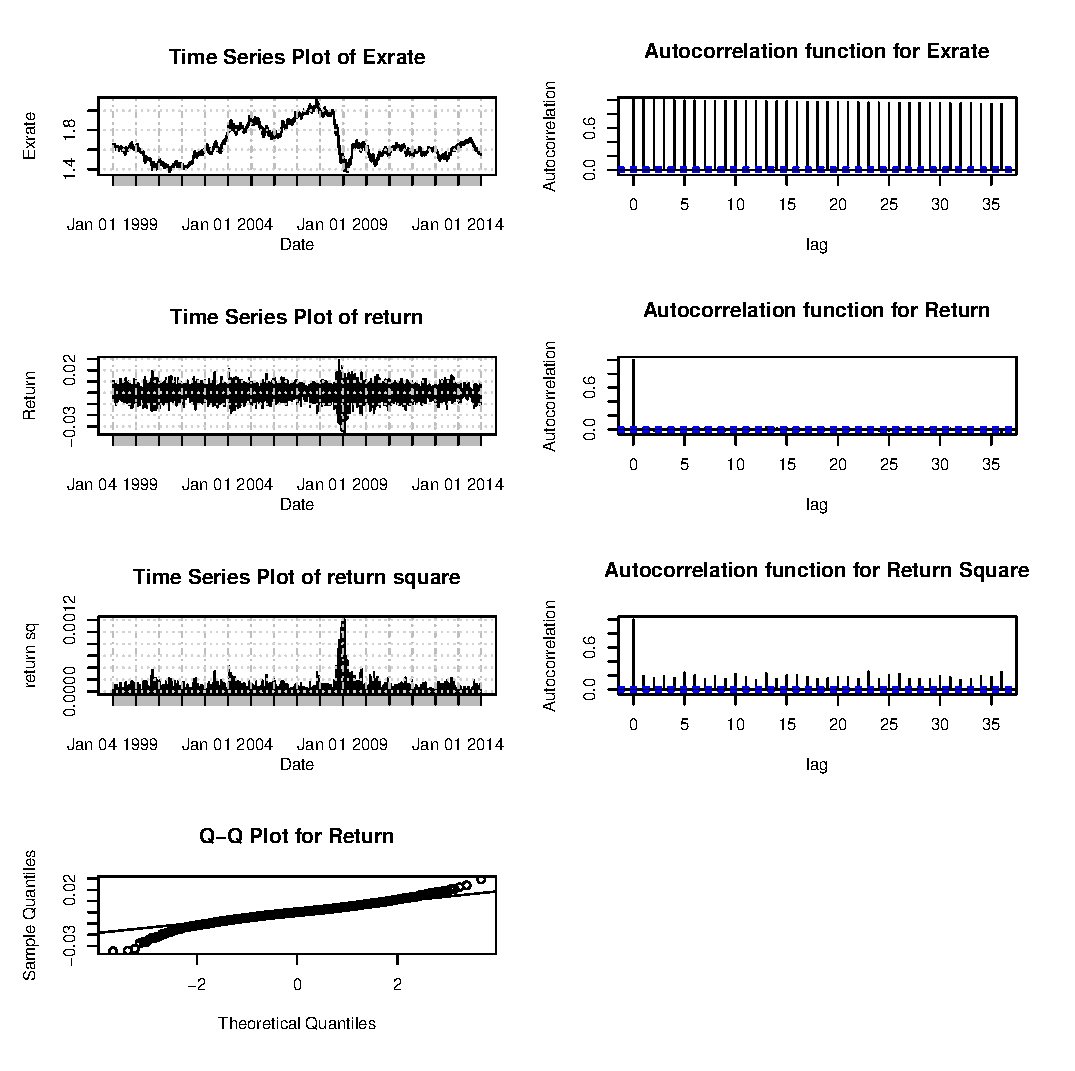
\includegraphics[width=\textwidth]{chapters/chapter_uvts/figures/31graphs.eps}
	\caption{Exchange rate related plots.\label{fig:exchrate}}
	\end{figure}

	\begin{figure}[!ht]
	\centering
	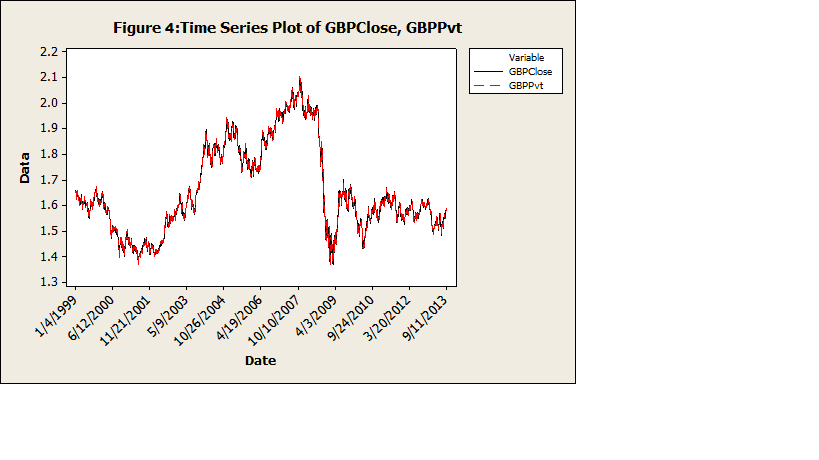
\includegraphics[width=\textwidth]{chapters/chapter_uvts/figures/Sec2-4Fig4.png}
	\caption{Times series plot of GBPClose, GBPPvt. \label{fig:timegbp}}
	\end{figure}
	
	\begin{figure}[!ht]
	\centering
	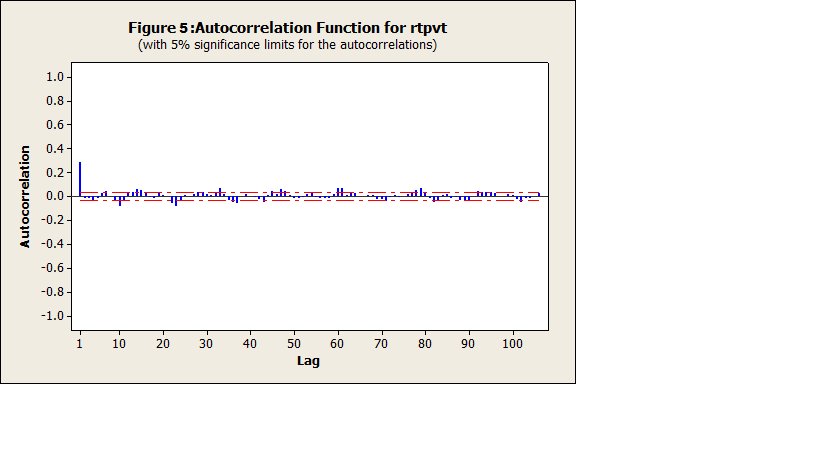
\includegraphics[width=\textwidth]{chapters/chapter_uvts/figures/Sec2-4Fig5.png}
	\caption{Autocorrelation function for rtpvt \label{fig:autocorrtpvt}}
	\end{figure}
An assumption of the random walk model that is often made is that the errors (returns)
follow a normal distribution. But in practice, the errors (or returns) tend to have heavier tails than the normal. We suggest using the quantile-quantile plot which is quite sensitive to even modest deviations from normality and also a test based on the properties of normal distribution. An omnibus test based on the skewness ($=0$ for normal) and the kurtosis ($=3$ for normal) is Jarque-Bera test:
	\begin{equation}\label{eqn:2JB}
	\text{JB }= n\left(\frac{\widehat{\text{SK}}^2}{6} + \frac{(\hat{K} - 3)^2}{24}\right) \sim \chi_2^2
	\end{equation}
where $\text{SK}\text{(ewness)}= E(\frac{X-\mu}{\sigma})^3, \text{K}\text{(urtosis)} = E(\frac{X-\mu}{\sigma})^4$. The corresponding sample numbers are substituted in JB (see Jarque and Bera (1980)\cite{jarque80}). The probability (Q--Q) plot of $r_t = \ln{(p_t)} - \ln{(p_{t-1})}$ as given in Figure 3 clearly indicates that the distribution has somewhat heavy tails. For this data $\widehat{SK} = -0.31$ and $\hat{K} = 3.67$ resulting in $\text{JB}= 129.7$ with $n= 3236$, thus rejecting the normal distribution. \\


\noindent\textbf{Stylized fact 2:} Heavy Tails: The returns are likely to display a heavy
tailed distribution such as a power-law or Pareto. \\


\noindent\textbf{Stylized fact 3:} Asymmetry: When prices fall, they tend to fall faster
than they tend to rise, thus drawdowns tend to be larger than upward rises. \\


These stylized facts are particularly important for risk management of strategies, and how they could be incorporated in trading decisions is still a subject of much research and will be discussed later.


\section{Time Series Models for Aggregated Data: Modeling the Variance}


In the ARMA$(p,q)$ model $\phi(B)Y_t= \delta + \theta(B) \,\varepsilon_t$ for series $\{Y_t\}$, when the errors $\varepsilon_t$ are \textit{independent} r.v.'s (with the usual assumptions of zero mean and constant variance $\sigma^2$), an implication is that the \textit{conditional} variance of $\varepsilon_t$ given the past information is a constant not depending on the past. This, in turn, implies the same feature for $l$-step ahead forecast errors $e_t(l) = \sum_{i=0}^{l-1}\psi_i\varepsilon_{t+l-i}$. However, in some settings, particularly for data from finance, the variability of errors may exhibit dependence on the past variability. Modeling the variance, which is essential for studying the risk-return relationship is an important topic in finance. \\


\noindent \textbf{Autoregressive Conditional Heteroscedastic (ARCH) Models} \\


The autoregressive conditional heteroscedastic (ARCH) models were originally proposed by Engle (1982)~\cite{engle1982}, Engle and Kraft (1983)~\cite{engle1983}, to allow for the conditional error variance in an ARMA process to depend on the past squared innovations, rather than be a constant as in ARMA models with independent errors. For example, an AR$(p)$ process with ARCH$(q)$ model errors is given as $Y_t = \sum_{i=1}^p\phi_iY_{t-i} + \delta + \varepsilon_t$, where,
	\begin{equation}\label{eqn:2ht}
	\begin{split}
	E&(\varepsilon_t\,|\,\varepsilon_{t-1},\varepsilon_{t-2},\cdots)= 0 \text{ and} \\
	h_t&= \Var(\varepsilon_t \,|\, \varepsilon_{t-1},\varepsilon_{t-2},\cdots) = E(\varepsilon_t^2\,|\,\varepsilon_{t-1},\varepsilon_{t-2},\ldots) = \omega_0 + \sum_{i=1}^q\omega_i\varepsilon_{t-i}^2
	\end{split}
	\end{equation}
with $\omega_0 > 0$ and $\omega_i \geq 0$ for $i= 1,\ldots,q$. In the generalized ARCH (GARCH) model, introduced by Bollerslev (1986)~\cite{bollerslev1986}, it is assumed that
	\begin{equation}\label{eqn:2secondht}
	h_t = E(\varepsilon_t^2|\varepsilon_{t-1},\varepsilon_{t-2},\cdots) = \omega_0 + \sum_{i=1}^q\omega_i\varepsilon_{t-i}^2 + \sum_{i=1}^k\beta_ih_{t-i},
	\end{equation}
where $\beta_i \geq 0$ for all $i = 1,\ldots,k$. Much subsequent research on and applications of the ARCH and GARCH models have occurred since the original research papers.


Let us briefly discuss some basic results and implications of the ARCH and GARCH models. The errors $\varepsilon_t$ in the model have zero mean, since $E(\varepsilon_t) = E[E(\varepsilon_t\,|\,\varepsilon_{t-1}\cdots)] = 0$, and they are serially uncorrelated; that is, $E(\varepsilon_t\varepsilon_{t-j}) = 0$ for $j \not= 0$ (since for $j > 0$, for example, $E(\varepsilon_t\varepsilon_{t-j}) = E[E(\varepsilon_t\varepsilon_{t-j}\,|\,\varepsilon_{t-1}\cdots)] = E[\varepsilon_{t-j}E(\varepsilon_t\,|\,\varepsilon_{t-1}\cdots)] = 0$). But the $\varepsilon_t$ are not mutually independent r.v.'s since they are inter-related through their conditional variances (i.e., their second moment). We will also assume that the $\varepsilon_t$ have equal unconditional variances, $\Var(\varepsilon_t) = \sigma^2$, for all $t$, so they are weakly stationary. Consider, then, the simple case of the first-order ARCH or ARCH(1) model,
	\begin{equation}\label{eqn:2htE}
	h_t = E(\varepsilon_t^2|\varepsilon_{t-1},\cdots) = \omega_0 + \omega_1\varepsilon_{t-1}^2,
	\end{equation}
Assuming that $\omega_1 < 1$ ($\omega_0$ and $\omega_1 \geq 0$ is always assumed), the \textit{unconditional} variance of $\varepsilon_t$ is $\sigma^2= \Var(\varepsilon_t) = \frac{\omega_0}{1 - \omega_1}$, since $\sigma^2 = E(\varepsilon_t^2) = E[E(\varepsilon_t^2|\varepsilon_{t-1},\cdots)] = E[\omega_0 + \omega_1\varepsilon_{t-1}^2] = \omega_0 + \omega_1\sigma^2$. Therefore, the conditional variance of $\varepsilon_t$ can be written as
	\begin{equation}\label{eqn:2htw}
	h_t = \omega_0 + \omega_1\varepsilon_{t-1}^2 = \sigma^2(1 - \omega_1) + \omega_1\varepsilon_{t-1}^2 = \sigma^2 + \omega_1(\varepsilon_{t-1}^2 - \sigma^2),
	\end{equation}
or in the form of deviation from the unconditional variance as $h_t - \sigma^2= \omega_1(\varepsilon_{t-1}^2 - \sigma^2)$. So the conditional variance will be above the unconditional variance whenever $\varepsilon_{t-1}^2$ exceeds its unconditional variance $\sigma^2$. If $\varepsilon_t$ were conditionally normally distributed, given the past, the fourth unconditional moment $E(\varepsilon_t^4)$ will exceed $3\sigma^4$ (the value in the normal distribution), so that the marginal distribution of $\varepsilon_t$ will exhibit fatter tails that the normal distribution. Conditional variances of multi-step ahead forecast errors can also be established to depend on the past squared errors. These basic results indicated for the ARCH(1) model also tend to hold for the higher order ARCH$(q)$ models. A basic impact of the ARCH errors in a process is in assessment of the accuracy of forecast, since the forecast errors will have conditional variances (given the past) that depend on the past. This allows for formation of correct and more informative (conditional) prediction intervals that would be obtained under the usual assumption that conditional error variances were constant independent of the past.


Now consider briefly the popular GARCH(1,1) model, $h_t = E(\varepsilon_t^2|\varepsilon_{t-1},\cdots) = \omega_0 + \omega_1\varepsilon_{t-1}^2 + \beta_1h_{t-1}$. Similar to the result for the ARCH(1) model, assuming that $\omega_1 + \beta_1 < 1$, it is readily shown that the unconditional variance of $\varepsilon_t$ is equal to $\sigma^2 = Var(\varepsilon_t) = \omega_0/[1 - (\omega_1 + \beta_1)]$. Let $v_t = \varepsilon_t^2 - h_t$, so that the r.v.'s $v_t$ have zero mean, and they are serially uncorrelated since
	\[
	\begin{split}
	E((\varepsilon_t^2 - h_t)(\varepsilon_{t-j}^2 - h_{t-j}))&= E[ E\{(\varepsilon_t^2 - h_t)(\varepsilon_{t-j}^2 - h_{t-j}) \,|\,\varepsilon_{t-1},\cdots\}] \\
	&= E[(\varepsilon_{t-j}^2 - h_{t-j}) E\{(\varepsilon_t^2 - h_t) \,|\,\varepsilon_{t-1},\cdots\}] = 0.
	\end{split}
	\]
Then, since $h_t = \varepsilon_t^2 - v_t$, note that the GARCH(1,1) model can be rearranged as $\varepsilon_t^2 - v_t = \omega_0 + \omega_1\varepsilon_{t-1}^2 + \beta_1(\varepsilon_{t-1}^2 - v_{t-1})$, or
	\begin{equation}\label{eqn:2ept}
	\varepsilon_t^2 = \omega_0 + (\omega_1 + \beta_1)\varepsilon_{t-1}^2 + v_t - \beta_1v_{t-1},
	\end{equation}
This form reveals that the process of squared errors, $\{\varepsilon_t^2\}$, follows an ARMA(1,1) model with uncorrelated innovations $v_t$ (however, the $v_t$ are conditionally heteroscedastic and more strongly are Martingale differences. Although this process looks like a linear process, it is not, since $ \{v_t\}$ are uncorrelated but dependent). This fact motivates the use of the ACF and PACF of the squares $\varepsilon_t^2$ for model specification and for basic preliminary checking for the presence of ARCH/GARCH effects in the errors $\varepsilon_t$. In practice, a starting point would be examination of the sample ACF and PACF of the squared residuals $\hat{\varepsilon}_t^2$, where $\hat{\varepsilon}_t$ are residuals obtained from fitting of a usual ARMA$(p,q)$ model (e.g., McLeod and Li, 1983~\cite{mcleod1983}). The correspondence between ARCH and ARMA is further noted via the condition, $0<\sum_{i=1}^q \omega_i<1$, that implies the roots of its characteristic equation lie outside the unit circle (like a causal ARMA).


For maximum likelihood (ML) estimation of models with ARCH or GARCH errors, assuming that $\varepsilon_t$ is conditionally normally distributed as $N(0,h_t)$, we have the log-likelihood function (apart from some initial conditions) given by $\log(L) = -\frac{T}{2} \log(2\pi) - \frac{1}{2}\sum_{t=1}^T \log(h_t) - \frac{1}{2}\sum_{t=1}^T \varepsilon_t^2/h_t$. Maximum likelihood estimation procedures, properties of the estimators, and Lagrange multiplier (LM) and likelihood ratio (LR) procedures for testing for the presence of ARCH effects in the conditional variances of the $\varepsilon_t$ have been considered by Engle (1982)~\cite{engle1982} and Weiss (1984) \cite{weiss1984}, among others.


As there are other excellent sources to learn about ARCH and GARCH models (see Tsay (2010)~\cite{tsay}, Ch 3), we have limited our discussion to some basic details. \\


\noindent\textbf{Preliminary Testing for ARCH Effect:} The test is the omnibus test similar to Ljung-Box test that examines the presence of autocorrelation up to certain number of lags, which is equivalent to testing, $H_0: \alpha_1 = \alpha_2 \cdots = \alpha_q = 0$ in the model
	\begin{equation}\label{eqn:2eptsq}
	\varepsilon_t^2 = \alpha_0 + \alpha_1\varepsilon_{t-1}^2 + \cdots + \alpha_q\varepsilon_{t-q}^2 + a_t
	\end{equation}
where $a_t$ is white noise series; note that $\{a_t\}$ does not need to follow a normal distribution. The usual $F$-test used in regression can be applied here; Let $R^2$ be the coefficient of determination that result from (\ref{eqn:}) when $\hat{\varepsilon}_t$'s are used; then
	\begin{equation}\label{eqn:2F}
	F = \frac{R^2/q}{(1 - R^2)/(T - 2q - 1)} \sim \chi^2/q
	\end{equation}
We use $\chi^2$ instead of $F$ due to the fact that $\varepsilon_t$'s are estimated quantities. More informally, one could use the ACF of $\hat{\varepsilon}_t^2$ and if any of the autocorrelations are out of the normal bounds, $\pm 2/\sqrt{T}$, we may examine further for ARCH effects. \\


\noindent\textbf{GARCH vs ARCH:} While ARCH models care for the time dependence in volatilities and have elegant properties such as having excessive kurtosis (matching the empirical finding related to asset returns), they tend to overpredict the volatility and treat both negative and positive, $\varepsilon_t$'s symmetrically. To overcome some of these issues and as well as to come up with a more parsimonious representation (as in AR vs ARMA considerations) GARCH models stated in (\ref{eqn:2ept}) are proposed. \\


\noindent\textbf{IGARCH:} The variance can persist for extended periods and can change at different time spans, thus leading to non-stationary behavior. In the GARCH(1,1) model, it is possible that $w_1 + \beta_1 = 1$, so that IGARCH(1,1) (Integrated GARCH) can be written as
	\begin{equation}\label{eqn:2eptsqrt}
	\varepsilon_t = \sqrt{h_t} \cdot a_t,\qquad h_t = w_0 + w_1h_{t-1} + (1 - w_1)\varepsilon_{t-1}^2
	\end{equation}
If $h_t$ is proxied by $\varepsilon_t^2$, the above model leads to $\varepsilon_t^2 - \varepsilon_{t-1}^2 = w_0 + w_1(\varepsilon_{t-1}^2 - \varepsilon_{t-2}^2)$, which is similar in form to non-stationary autoregressive model. In practice because of level shifts in volatility, IGARCH appears to be a natural model to fit. Because the IGARCH(1,1) is similar to ARIMA(0,1,1), the model can be taken as an exponential smoothing model for the $\varepsilon_t^2$ series; By iterative substitutions, we can show that
	\begin{equation}\label{eqn:2ht1w}
	h_t = (1 - w_1)(\varepsilon_{t-1}^2 + w_1\varepsilon_{t-2}^2 + w_1^2\varepsilon_{t-3}^2 \cdots)
	\end{equation}
where $w_1$ can be taken as a discount factor. \\


\noindent\textbf{Prediction Performance of GARCH:} The predictive power of GARCH based on ex-post forecast evaluation criteria tend to suggest that the model provide poor forecasts, although the in-sample parameter estimates turn out to be highly significant. As Andersen and Bollerslev (1998)~\cite{andersen1998} note, in the model (\ref{eqn:2ept}), the latent volatility, $h_t$, evolves over time. The approach to evaluate the performance of the model for $h_t$ via $\hat{\varepsilon}_t^2$ is not appropriate. While $\hat{\varepsilon}_t^2$ provides an unbiased estimate of $h_t$, it is a noisy measurement due to idiosyncratic error terms associated with it; these error terms maybe due to the result of compounding frictions in the trading process. This will be clarified when we discuss the analysis of high-frequency data. \\


\noindent \textbf{Time--Varying ARCH Processes (tvARCH):} The underlying assumptions of ARCH models is stationarity and with changing pace of economic conditions the assumption of stationarity is not appropriate for modeling financial returns over long intervals. We may obtain a better fit by relaxing the assumption of stationarity. Dahlhaus and Subba Rao (2006)~\cite{dahlhaus2006} generalize the ARCH model with time-varying parameters:
	\begin{equation}\label{eqn:2eptsqrtht}
	\varepsilon_t = \sqrt{h_t}\cdot a_t,\quad h_t = w_0(t) + \sum_{j=1}^{\infty}w_j(t)\varepsilon_{t-j}^2
	\end{equation}
which $a_t$'s are i.i.d. with mean zero and variance, one. By rescaling the parameters to unit intervals, the tvARCH process can be approximated by a stationary ARCH process. A broad class of models resulting from (\ref{eqn:}) can be stated as:
	\begin{equation}\label{eqn:2eptN}
	\varepsilon_{t,N} = \sqrt{h_{t,N}}\cdot a_t,\quad h_{t,N} = w_0\left(\frac{t}{N}\right) + \sum_{j=1}^pw_j \left(\frac{t}{N}\right) \varepsilon_{t-j,N}^2
	\end{equation}
for $t= 1,2,\ldots,N$. This model captures the slow decay of the sample autocorrelations in squared returns that is commonly observed in financial data which is attributed to the long memory of the underlying process. But tvARCH$(p)$ is a non-stationary process that captures the property of long memory.


Fryzlewicz, Sapatinas and Subba Rao (2008)~\cite{fryzlewicz2008} propose a kernel normalized-least squares estimator which is easy to compute and is shown to have good performance properties. Rewriting (\ref{eqn:2eptN}) as
	\begin{equation}\label{eqn:2eptNsq}
	\varepsilon_{t,N}^2 = w_0\left(\frac{t}{N}\right) + \sum_{j=1}^p w_j\left(\frac{t}{N}\right)\varepsilon_{t-j,N}^2 + (a_t^2 - 1)h_{t,N}^2
	\end{equation}
in the autoregressive form, the least squares criterion with the weight function, $k(u_0,\chi_{k-1,N})$, where $\chi_{k-1,N}' = (1,\varepsilon_{k-1,N}^2,\ldots,\varepsilon_{k-p,N}^2)$ is
	\begin{equation}\label{eqn:2Lt0}
	L_{t_0,N}(\alpha) = \sum_{k=p+1}^N \frac{1}{b_N} \;w\left(\frac{t_0-k}{b_N}\right) \frac{\left(\varepsilon_{k\cdot N}^2 - \alpha_0 - \sum_{j=1}^p\alpha_j\varepsilon_{k-j\cdot N}^2\right)^2}{k(u_0, \chi_{k-1\cdot N})^2}
	\end{equation}
Minimizing (\ref{eqn:2Lt0}) yields, $\hat{a}_{t_0,N} = R_{t_0,N}^{-1}r_{t_0,N}$ where
	\begin{center}
	\begin{flalign}\label{eqn:2Rt0}
	&& R_{t_0,N}&= \sum_{k=p+1}^N \frac{1}{b_N}\ ; w\left(\frac{t_0-k}{b_N}\right) \frac{\chi_{k-1\cdot N}\chi_{k-1\cdot N}'}{k(u_0,\chi_{k-1\cdot N})^2} && \notag \\
	\text{and} && \phantom{x} & \phantom{x} && \\
	&& r_{t_0,N} &= \sum_{k=p+1}^N\frac{1}{b_N}\; w\left(\frac{t_0-k}{b_N}\right)\frac{\varepsilon_{k\cdot N}^2\chi_{k-1\cdot N}}{k(u_0,\chi_{k-1\cdot N})^2} && \notag
	\end{flalign}
	\end{center}
The kernel $w$ is a function defined on $[-\frac{1}{2},\frac{1}{2}]$ which is of bounded variation. The choice of weight function suggested is as follows: it is motivated by the differing variances at various values of $k$. Estimate,
	\begin{center}
	\begin{flalign}\label{eqn:2skN}
	&& \hat{\mu}_{t_0,N}&= \sum_{k=1}^N\frac{1}{b_N} \; w\left(\frac{t_0 - k}{b_N}\right)\varepsilon_{k\cdot N}^2 && \notag \\
	\text{and} && \phantom{x} & \phantom{x} && \\
	&& s_{k-1\cdot N} &= \sum_{j=1}^p\varepsilon_{k-j\cdot N}^2 && \notag
	\end{flalign}
	\end{center}
and use $k_{t_0,N}(s_{k-1},N) = \hat{\mu}_{t_0,N} + s_{k-1\cdot N}$ as the weight function. Thus the estimation is a two-stage scheme. For the bandwidth selection, the cross-validation method based on a subsample of the observations is suggested.


The methodology presented here is useful because of the changing nature of financial volatility. Real data applications will be discussed in Chapter 3.


\section{Stylized Models for Variance of Asset Returns}


Volatility has many important implications in finance. It is one of the most commonly
used risk measure and plays a vital role in asset allocation. The estimate of volatility of an asset is obtained using the prices of stock or options or both. Three different measures that are normally studied are stated below:
\begin{itemize}
\item Volatility is the conditional standard deviation of daily or low frequency returns.

\item Implied volatility is derived from options price under some assumed
relationship between the options and the underlying stock prices.

\item Realized volatility is an estimate of daily volatility using high frequency
intraday returns.
\end{itemize}
In this section we will mainly focus on the first item and the others will be discussed in a later section on high frequency data.


Consider $r_t = \ln{(p_t) - \ln{(p_{t-1})}}$, return of an asset. We observed that `$r_t$' exhibits no serial correlation. This does not imply that the series `$r_t$' consists of independent observations. The plot of $r_t^2$ given in Figure~\ref{fig:} clearly indicates that volatility tends to cluster over certain time spans. The autocorrelations in Figure~\ref{fig:} confirms that there is some time dependence for the volatility. In fact, there is some long range dependence that spans up to sixty days. \\


\noindent\textbf{Stylized fact 4:} Volatility clustering: High volatility events tend to cluster in time and this can be measured through positive correlations that exist over several lags.


To formally model the volatility, recall the conditional mean and the conditional variance of the return, $r_t$, are: $\mu_t = E(r_t \,|\,F_{t-1}),\sigma_T^2 = \Var(r_t\,|\,F_{t-1}) = E((r_t - \mu_t)^2\,|\,F_{t-1})$.


We have observed for the exchange rate series that $\mu_t \approx$ constant and is generally
close to zero. But $\sigma_t^2$ clusters around certain time spans and modeling variation
in $\sigma_t^2$ is typically done through ARCH/GARCH models and also through
stochastic volatility models. The stochastic volatility models have the advantage of modeling jumps in prices that are also often used in derivative pricing. To begin with, we can test for the heteroscedasticity using the test in (\ref{eqn:2F}) or one of the following which are all equivalent asymptotically:
\begin{itemize}
\item \textbf{Ljung-Box Omnibus Test:}
	\begin{equation}\label{eqn:2Qk}
	Q_k = T(T+2) \cdot \sum_{j=1}^k\frac{(\hat{e}^{j})^2}{T - j} \sim \chi_{k-m}^2
	\end{equation}
where $\hat{e}^{(j)}$ is the $j$th lag autocorrelation of $r_t^2$; $m$ is the number of independent parameters. Here $H_0: \rho_1 = \rho_2 = \cdots \rho_k = 0$.

\item \textbf{Lagrange Multiplier Test:} Regress $r_t^2$ on $r_{t-1}^2,\ldots,r_{t-q}^2$ and obtain $R^2$ the coefficient of determination; Test the $H_0$: Slope coefficients are all zero, by
	\begin{equation}\label{eqn:2TstarR}
	T \cdot R^2 \sim \chi_q^2
	\end{equation}
\end{itemize}
These tests were carried out on the exchange rate data; Table~\ref{tab:box} has the result of Ljung-Box Test: 
\begin{table}[!ht]
\centering
\caption{Ljung-Box Chi-Square Statistics for Exchange rate data \label{tab:box}}
	\begin{tabular}{ccccc}
	 h & 12 & 24 & 36 & 48 \\ \hline
	$Q_h$ & 73.2 & 225.7 & 463.4 & 575.7 \\ \hline
	df & 6 & 18 & 30 & 42 \\ \hline
	$p$-value & 0.000 & 0.000 & 0.000 & 0.000 \\
\end{tabular}
\end{table}


The Lagrange Multiplier test with $q=5$ also gives $R^2= 0.065$, that $T\cdot R^2= 243.6$ and compared with $\chi_5^2$ table values has $p$-value $\approx$ 0. These results clearly confirm that there is some time dependence in the volatility.


Among the conditional heteroscedasticity models ARCH/GARCH that were discussed in the last section, GARCH is simple to use and also results in more parsimonious modeling. Therefore, we present only the estimated GARCH model here. For exchange rate data, the estimated GARCH model is $\hat{\sigma}_t^2 = 2.61 \times 10^{-7} + 0.037r_{t-1}^2 + 0.95\hat{\sigma}_{t-1}^2$. Observe that the coefficients $r_{t-1}^2$ and $\hat{\sigma}_{t-1}^2$ add up to unity approximately and thus indicating the volatility is best modeled through IGARCH, which seems to hold generally for many asset volatilities.


\section{A Model for Volume-Volatility Relationship}


While the price information via returns and the volatility can be modeled through methods described earlier, it has become important to incorporate other relevant trading data to augment the trading strategies. To that effect, we want to seek some guidance from economic theory how that information is linked to price movements.

In the market microstructure theory, it is assumed that price movements occur primarily due to the arrival of new information and this information is incorporated efficiently into market price. Other variables such as trading volume, bid-ask spread and market liquidity are observed to be related to the volatility of the returns. Early empirical studies have documented a positive relationship between daily trading volume and volatility (See Clark (1973)~\cite{clark}). Epps and Epps (1976)~\cite{epps} and Tauchen and Pitts (1983)~\cite{tauchenpitts} assume that the volume and price are driven by the underlying `latent' information ($I$) and provide a theoretical framework to incorporate this information. Assuming that there are fixed number of traders who trade in a day and the number of daily equilibria, $I$ is random because the number of new pieces of information is random, the return and the volume are written as a bivariate normal mixture model with the same mixing variable $I$. Conditional on $I$:
	\begin{equation}\label{eqn:2rtVt}
	\begin{split}
	 r_t&= \sigma_1\sqrt{I_t}Z_{1t} \\
	 V_t&= \mu_VI_t + \sigma_2\sqrt{I_t}Z_{2t}
	 \end{split}
	 \end{equation}
where $Z_{1t}$ and $Z_{2t}$ are standard normal variables and $Z_{1t}, Z_{2t}$, and $I_t$ are mutually independent. Thus the volatility-volume relationship,
	\begin{equation}\label{eqn:2covVt}
	\begin{split}
	\Cov(r_t^2,V_t)& = E(r_{t}^2V_t) - E(r_t^2) \,E(V_t) \\ 
	&= \sigma_1^2\mu_V \Var(I_t) > 0
	\end{split}
	\end{equation}
is positive due to the variance in $I_t$. If there is no new information or if there is no variation in the mixing variable, $\Var(I_t)= 0$ and thus the relationship vanishes. The theory of arrival rates suggest a
Poisson distribution and based on empirical evidence, the lognormal distribution is taken to be a candidate for distribution of mixing variable, $I_t$. The parameters of the model in (\ref{eqn:2rtVt}) are estimated through maximum likelihood. Gallant, Rossi and Tauchen (1992)~\cite{grt} using a semi-parametric estimate of the joint density of $r_t$ and $V_t$ conduct a comprehensive study of NYSE data from 1925 to 1987. The following summarizes their findings: \\


\noindent\textbf{Stylized Facts 5 (Volume--Volatility Relationship):} 

\begin{itemize}
\item  Positive correlation between conditional volatility and volume.

\item Large price movements are followed by high volume.

\item Conditioning on lagged volume substantially attenuates the leverage (which is an asymmetry in the conditional variance of current price change against past price change) effect.

\item After conditioning on lagged value, there is a positive risk-return relation.
\end{itemize}


Andersen (1996)~\cite{andersen} modifies the model (\ref{eqn:2rtVt}) by integrating the microstructure
setting of Glosten and Milgrom (1985)~\cite{glostenmilgrom} with the stochastic volatility, that is built on weaker conditions on the information arrival process. While the first equation in (\ref{eqn:2rtVt}) remains the same, the volume $V_t$ has informed and noise components, $V_t = IV_t + NV_t$. Noise trading component, $NV_t$ is taken as a time homogeneous Poisson process, $P_0(m_0)$. Therefore, the systematic variation in trading is mainly due to informed volume. Then $IV_t|I_t \sim \text{Poisson}(I_t\mu)$ and thus
	\begin{equation}\label{eqn:2VtIt}
	V_t|I_t \sim \text{Poisson}(m_0 + I_t m_1)
	\end{equation}
It is easy to see $\Cov(r_t^2,V_t) = \sigma^2m_1 \Var(I_t) > 0$ under this setting as well. These models clearly indicate that the intraday return volatility and volume processes jointly contain predictable elements.


There are other studies that focus on the trading volume and returns relationship and we mention only a select few here. Campbell, Grossman, and Wang (1993)~\cite{campbellgross} demonstrate for individual large stocks and stock indices the first-order daily auto-correlation in the returns tend to decline with volume. The authors develop a theoretical model where the economy has two assets, risk-free asset and a stock and there are two types of investors, one with constant risk aversion and the other with risk aversion changing over time. Under this set-up, it is implied that a decline in a stock price on a high-volume day is more likely than a decline on a low-volume day to be associated with an increase in the expected stock return.


Gervais, Kaniel, and Mingelgrin (2001)~\cite{gervais2001high} investigate the role of trading activity in providing information about future prices. It is shown that periods of extremely high (low) volume tend to be followed by positive (negative) excess returns. The formation period for identifying extreme trading volume is a day or a week, but the effect lasts at least twenty days and holds across all stock sizes. To test if this information can be used profitably, the authors construct a trading strategy, by sending buy (sell) limit orders at the existing bid (ask) price, at the end of the formation period. If the orders are not taken, they are converted into market orders at the closing. The strategy is shown to result in profits, in particular with the small-medium firm stocks, after adjusting for the transaction costs. The model used for the empirical framework is the vector autoregressive model discussed later, with an addition of a set of exogenous control variables:
	\begin{equation}\label{eqn:2Ytphi}
Y_t = \Phi_0+\sum_{j=1}^p\Phi_jY_{t-j}+\sum_{l=1}^LB_lX_{t-l}+\epsilon_t
	\end{equation}


The components of $Y_t$ include stock or market related variables such as detrended log of stock turnover, the stock return and the value weighted market return. The control variables are market volatility based on the daily return standard deviation and the dispersion which is the cross-sectional standard deviation of the security returns. The impulse response functions are used to aggregate the overall relationship among the endogenous variables. Statman, Thorley, and Vorkink (2006)~\cite{statman2006investor} show that the trading volume is dependent on past returns over many months and it is argued that this may be due to the overconfidence of the investors.


These and other studies generally confirm the information content of the volume and turnover of stocks traded; strategies to exploit these, especially in a high frequency context, will be examined in Chapter 3. We will discuss how intra-day flow of volume can be related to price changes. 


In algorithmic trading a key ingredient of many strategies is forecast of intra-day volume. Typically a parent order is split into several child orders and the timing of the submission of child orders could depend on the volume forecast for an interval of time that is considered for trading. Brownless, Cipollini and Gallo (2011)~\cite{brownless} provide prediction model for intra-day volume. This will be described in detail in the next chapter.


\section{Regime Switching and Change-Point Models}


It has been long noted in finance that there are two kinds of recurrences in stock prices: underreaction and overreaction to a series of good or bad news. The securities that have a good record for an extended period tend to become overpriced and have low returns subsequently. Barberis, Shleifer and Vishny (1998)~\cite{vishny} present a model where investor believes that the returns can arise from one of two regimes although returns follow random walk: mean-reverting or trending. The transition probabilities are taken to be fixed and the regime is more likely to stay the same rather than to switch. But the investor's beliefs are updated as and when the returns data are observed. It is presumed that in many instances, we may not discern these shifts directly whether or when they occur but instead can draw probabilistic inference based on the observed behavior posthumously. Hamilton (2016)~\cite{jdham} reviews models for regime-switching applied in several contexts in macroeconomics, building upon the elegant model introduced in Hamilton (1989)~\cite{89ham}. Here in this section, we will cover only studies that are relevant to finance applications, particularly relevant to trading that exploit anomalies. 


Consider the model,
	\begin{equation}\label{eqn:modelham}
	y_t = \mu_{s_t} + \epsilon_t, \quad s_t=1,2
	\end{equation} 
where $y_t$ is the observed variable, such as asset return and $s_t$ represents two distinct regimes and $\epsilon_t$'s are i.i.d.$\sim N(0,\sigma^2)$. Let $\{F_{t-1}\}$ be the information set available as of `$t-1$'. The transition between the regimes is taken to be Markovian,
	\begin{equation}\label{eqn:markprob}
	\text{Prob}(s_t=j \;|\; s_{t-1}=i, F_{t-1})= p_{ij}, \quad i,j=1,2
	\end{equation}
thus leading to an AR(1) model for $\mu_{s_t}$ as
	\begin{equation}\label{eqn:must}
	\mu_{s_t} = \phi_0 + \phi_1 \mu_{s_{t-1}} + a_t
	\end{equation}
where $a_t$ by definition can take four possible values depending upon $s_t$ and $s_{t-1}$. Here $\phi_0=p_{21}\mu_1 + p_{12} \mu_2$ and $\phi_1=p_{11}-p_{21}$. Note the model for $y_t$ in (\ref{eqn:modelham}) is the sum of an AR(1) process and white noise, then from Theorem~\ref{thm:agg}, $y_t \sim$ ARMA(1,1); but because of discrete nature of `$a_t$', (\ref{eqn:modelham}) is a non-linear process. Note that the unknown parameters are $(\mu_1,\mu_2,\sigma,p_{11},p_{22})'=\lambda$ and they can be estimated via maximum likelihood as follows: note $y_t|(s_t=j,F_{t-1})\sim N(\mu_j,\sigma^2)$. The predictive density of $y_t$ is given as,
	\begin{equation}\label{eqn:predden}
	f(y_t \;|\; F_{t-1})= \sum_{i=1}^2 \text{Prob}(s_t=i \;|\; F_{t-1}) \, f(y_t \;|\; s_t=i, F_{t-1})
	\end{equation}
and estimate of $\lambda$ is obtained by maximizing the likelihood function $L(\lambda)=\sum_{t=1}^T \log f(y_t \;|\; F_{t-1}, \lambda)$. Two useful quantities are: \\


\noindent Predicted regime: 
	\begin{equation}\label{eqn:predreg}
	\text{Prob}(s_t=j \;|\; F_{t-1})= p_{1j} \text{Prob}(s_{t-1}=1 \;|\; F_{t-1}) + p_{2j} \,\text{Prob}(s_{t-1}=2 \;|\; F_{t-1})
	\end{equation}
\noindent Optimal forecast:
	\begin{equation}\label{eqn:optfore}
	E(y_t \;|\; F_{t-1})= \sum_{i=1}^2 (\phi_0+\phi_1 \mu_i) \text{Prob}(s_{t-1}=i \;|\; F_{t-1}).
	\end{equation}
The forecast for `$k$' period ahead can be stated as:
	\begin{equation}\label{eqn:period}
	E(y_{t+k} \;|\; F_{t-1}) = \mu+\phi_1^k \sum_{i=1}^2 (\mu_i-\mu)\, \text{Prob}(s_t=i \;|\; F_{t-1})
	\end{equation}
where $\mu=\phi_0/(1-\phi_1)$.


The basic model has been extended to cover multiple regimes and to vector processes. Interested readers should refer to Hamilton (2016)~\cite{jdham} and references therein. Ang and Timmermann (2012)~\cite{timmerman} discuss a model that accounts for changes not only in the mean but also in variances and autocorrelations:
	\begin{equation}\label{eqn:varautoy}
	y_t= \mu_{s_t} + \phi_{s_t} y_{t-1} + \epsilon_t
	\end{equation}
where $\epsilon_t$'s are independent $\sim N(0,\sigma_{s_t}^2)$. Using the data on excess S\&P500 returns, FX returns, etc., it is identified that there are volatility regimes, but no level shifts.


Hamilton (1990)~\cite{90ham} proposes using EM (Expectation-Maximization) algorithm (Dempster, Laird and Rubin (1977)~\cite{dempster}) to obtain the maximum likelihood estimate, instead of recursive filter approach (see Hamilton (1989)~\cite{89ham} to optimize the loglihood of (\ref{eqn:predden}), updated with $y_t$. Note by Bayes' Theorem
	\begin{equation}\label{eqn:bayes}
	\text{Prob}(s_t=j \;|\; F_t) = \dfrac{\text{Prob}(s_t=j \;|\; F_{t-1}) \, f(y_t\;|\; s_t=j, F_{t-1})}{f(y_t \;|\; F_{t-1})}
	\end{equation}
To get an estimate of $p_{ij}$ in step `$l+1$', use 
	\begin{equation}\label{eqn:hatpijl}
	\hat{p}_{ij}^{(l+1)}= \dfrac{\sum_{t=1}^{T-1} \text{Prob}(s_t=i, s_{t+1}=j \;|\; F_t, \hat{\lambda}^{(l)})}{\sum_{t=1}^{T-1} \text{Prob}(s_t=i \;|\; F_t, \hat{\lambda}^{(l)})}
	\end{equation}
and with these estimates obtain the ML estimates of the rest of the parameters ($\mu_1$, $\mu_2$, and $\sigma$) by maximizing the likelihood function. More details can be found in Hamilton (1990)~\cite{90ham}.


There is a vast literature on Bayesian approach to this problem, see for example, Chib (1998)~\cite{chib} and subsequent publications that followed. An interesting application is given in Pastor and Stambaugh (2001)~\cite{pastor}. Lai and Xing (2013)~\cite{laixing} study a general model, somewhat similar to (\ref{eqn:varautoy}):
	\begin{equation}\label{eqn:arxgarch}
	\text{ARX-GARCH:} \quad y_t= \beta_t' x_t + v_t \sqrt{h_t} \, \epsilon_t
	\end{equation}
where $h_t\sim$ GARCH$(p,q)$ and $\beta_t$ and $v_t$ are piecewise linear. Using the weakly returns of S\&P500 index, AR(1)-GARCH(1,1) model is attempted and it is identified that 1998--2003 had higher volatility. Figure~\ref{fig:sp500} provides the plot of closing price, returns, volatility and volume data. 


	\begin{figure}[!ht]
	\centering
	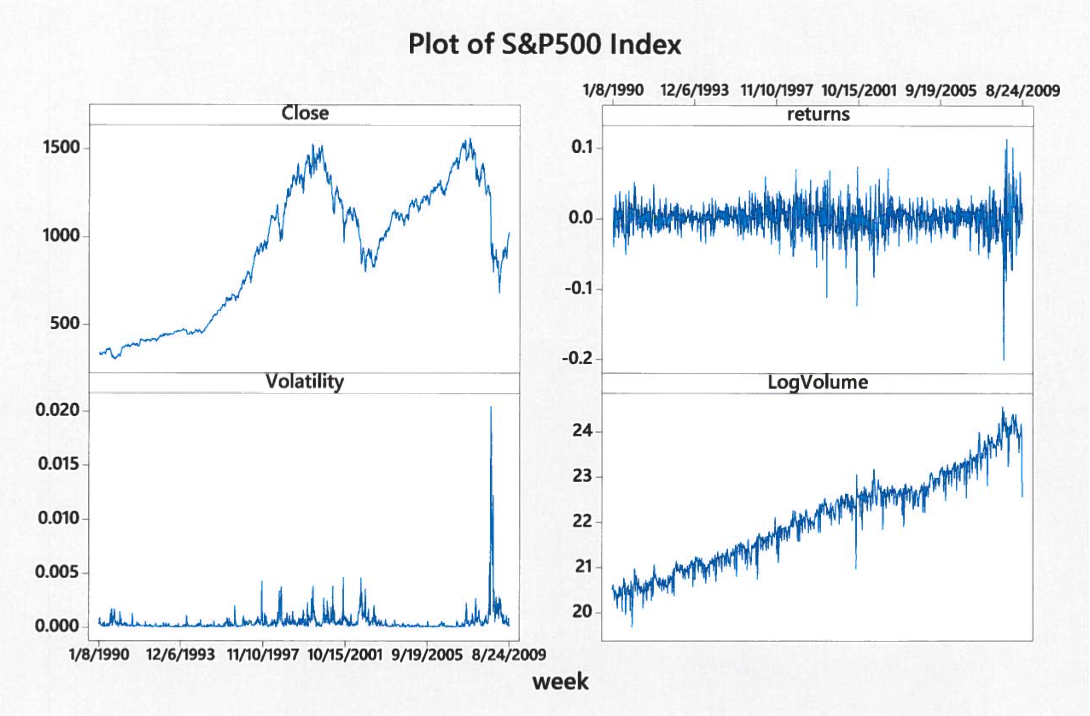
\includegraphics[width=\textwidth]{chapters/chapter_uvts/figures/sp500.png}
	\caption{Plot of S\&P 500 Index. \label{fig:sp500}}
	\end{figure}


In most of the applications of the above regime-switching models, particularly in finance, the plots of relevant quantities clearly reveal the pattern and these models provide a way to confirm the level and size shifts. We want to conclude this section with some simple ideas borrowed from the area of statistical process control. Recall that if the market is efficient, the return $r_t=\ln P_t - \ln P_{t-1}\sim $ IID $(\mu_t, \sigma^2)$, but $\mu_t=\delta$ when $t\geq t_0$ and zero elsewhere. The cumulative sum chart (CUSUM) to detect the positive and negative mean shift are based on recursive calculations:
	\begin{equation}\label{eqn:cdouble}
	\begin{split}
	c_t^+&=\max(0,c_{t-1}^+ + (r_t-k)) \\
	c_t^-&=\min(0,c_{t-1}^- - (r_t-k))
	\end{split}
	\end{equation}
where $k=\delta/2$. The chart signals as sown as $c_t^+$ reaches `$h$'---a decision point set by the user. Jiang, Shu and Apley (2008)~\cite{shuap} modify (\ref{eqn:cdouble}) with exponentially weighted moving average (EWMA) type of estimates that is adaptive in nature. It can be stated as,
	\begin{equation}\label{eqn:elma}
	s_t^+=\max\left(0,s_{t-1}^+ + w(\hat{\delta}_t)\left(r_t - \frac{\hat{\delta}_t}{2}\right)\right)
	\end{equation}
where $w(\hat{\delta}_t)$ is a weight function; a simple weight function $w(\hat{\delta}_t)=\hat{\delta}_t$ is suggested. The $\delta_t$ is updated as 
	\begin{equation}\label{eqn:updatedelt}
	\hat{\delta}_t=(1-\lambda)\, \hat{\delta}_{t-1} + \lambda r_t
	\end{equation}
The adaptive CUSUM chart is effective at detecting a range of mean shift sizes. Similar results for the variance need to be worked out.


In practical applications of these regime-shifting models, it is not easy to discuss between a single ??? and persistent level shift. Valid measures that can distinguish these two situations on a timely basis could be very valuable to a trader. 





\section{Multiple Time Series Modeling and Co-integration}

\subsection{Introduction}


Multiple time series analysis is concerned with modeling and estimation of dynamic relationships among m related time series $y_{1t},\ldots,y_{mt}$, based on observations on these series over $T$ equally spaced time points $t=1,...,T$, and also between these series and potential exogenous time series variables $x_{1t},\ldots,x_{nt}$, observed over the same time period. We shall explore the use of these techniques in statistical arbitrage in leveraging multiple markets in Chapter 3. We first introduce a general model for multiple time series modeling, but will specialize to vector autoregressive (VAR) models for more detailed investigation. As some concepts are similar to those of the univariate models discussed in Section 2.3, the presentation will be brief.


Let $Y_t=(y_{1t},\ldots, y_{mt})'$ be an $m \times 1$ multiple time series vector of response variables and let $X_t=(x_{1t}, \ldots, x_{nt})'$ be an $n \times 1$ vector of input or predictor time series variables. Let $\epsilon_t$ denote an $m \times 1$ white noise vector of errors, independently distributed over time with $E(\epsilon_t)=0$ and $\Cov(\epsilon_t)=\Sigma_{\epsilon\epsilon}$, a positive-definite matrix. We consider the multivariate time series model
	\begin{equation}\label{eqn:2ytcs}
	Y_{t} = \sum_{s=0}^{p}C_sX_{t-s}+\epsilon_t 
	\end{equation}
where the $C_s \text{ are } m\times n$ matrices of unknown parameters. In the general setting, the `input' vectors $X_t$ could include past (lagged) values of the response series $Y_t$. In the context of trading $Y_t$ could denote the prices of related assets, $X_{t-s}$ could represent the past values of $Y_t$ and the values of volume, volatility, market, industry factors, etc. Note that the model (\ref{eqn:2ytcs}) can be written in the form of a multivariate regression model. An important issue that arises in the multiple series modeling is as follows: even for moderate values of the dimensions $m$ and $n$, the number of parameters that must be estimated in model (\ref{eqn:2ytcs}), when no constraints are imposed on the matrices $C_s$ can become quite large. Because of the potential complexity of these models, it is often useful to consider canonical analyses or other dimension reduction procedures such as reduced-rank regression methods described in Reinsel and Velu (1998)~\cite{velurein}. This may also lead to more efficient models due to the reduction in the number of unknown parameters.


The class of models stated in (\ref{eqn:2ytcs}) is rather flexible and provides many options for modeling multivariate time series data. Specifically consider the VAR$(p)$ model,
	\begin{equation}\label{eqn:ytphi0}
	Y_{t} = \Phi_0 + \sum_{j=1}^{p}\Phi_jY_{t-j}+\epsilon_t 
	\end{equation}
with `$p$' lags. As in Section 2.3, we can define the mean, variance, and autocovariance functions for stationary series as follows; in addition we have the cross-correlation matrix that captures the leading relationships among all `$m$' series.
\begin{align*}
            \text{Mean:\qquad} & \mu= E(Y_t)\\
            \text{Variance:\qquad} & \Gamma(0)= E[(Y_t-\mu)(Y_t-\mu)']\\
            \text{Autocovariance:\qquad} & \Gamma(l)= E[(Y_t-\mu)(Y_{t-l}-\mu)']\\
            \text{Cross-correlation:\qquad} & \rho(l) = D^{-1}\Gamma(l) D^{-1}
\end{align*}
Here $D$ is the diagonal matrix of size $m \times m$, consisting of the `$m$' standard deviations taken from the variance terms, from the diagonal of $\Gamma(0)$. It is easy to observe,  $\Gamma(l)= \Gamma(-l)'$ and $\rho(l)=\rho(-l)'$. The linear dependence among all the variables in terms of leads-lags is fully captured by examining $\rho_{ij}(l)$. There are excellent sources to study about modeling multiple time series (see Tsay (2010)~\cite{tsay} and Reinsel (2002)~\cite{2002reinsel}). We focus mainly on the use of Vector AR$(p)$ (VAR$(p)$) model in studying the relationships among stocks or markets; we elaborate on them below.


Using the back-shift operator $B$, the model (\ref{eqn:ytphi0}), VAR$(p)$ can be written as, $ \Phi(B)Y_t=\Phi_0+\epsilon_t$, where $\Phi(B)=I-\Phi_1B-\cdots-\Phi_pB^p$ is a matrix polynomial. It can be shown for the process $Y_t$ to be stationary, the roots of $\left| \Phi(\lambda)-I \right|=0$ should all lie outside the unit circle. If $Y_t$ is stationary, then $\mu=[\Phi(1)]^{-1}\Phi_0$ where $\Phi(1)=I-\Phi_1-\cdots-\Phi_p$. An easy consequence of this form is the result of the Yule-Walker equations, which are useful to identify, $\Phi$'s, the autoregressive coefficients from the moment conditions:
	\begin{equation}\label{eqn:2gammarho}
	\begin{split}
	\Gamma(l)&= \Phi_1 \,\Gamma(l-1) +\cdots + \Phi_p\, \Gamma(l-p) \\
	\rho(l)&= \Phi_1^* \,\rho(l-1) + \cdots + \Phi_p^* \, \rho(l-p) 
	\end{split}
	\end{equation}
Here $\Phi_i^*=D^{-\frac{1}{2}}\Phi_iD^{-\frac{1}{2}}$. A general approach to building a VAR model is to sequentially increase the lag value, `$p$' and check if the added lag is significant. The lag coefficients are estimated from (\ref{eqn:2gammarho}) with their sample counter-parts and they provide good initial estimates. The VAR($p$) model building at the $i$th stage is fitting the model, $Y_t=\Phi_0+\Phi_1Y_{t-1}+\cdots+\Phi_iY_{t-i}+\epsilon_t$ via least-squares method and estimate the residual covariance matrix via
	\begin{equation}\label{eqn:2hatsigma}
	\hat{\Sigma_i} = \left(\frac{1}{T-2i-1} \right) \sum_{t=i+1}^{T}\Hat{\epsilon_t}^{(i)}{{\hat{\epsilon_t}^{(i)^\prime}}}, \qquad i \geq 0
	\end{equation}
where $ \Hat{\epsilon}_t^{(i)}=Y_t-\Hat{\Phi}_0^{(i)}-\Hat{\Phi}_1^{(i)}Y_{t-1}-...-\Hat{\Phi}_i^{(i)}Y_{t-i}$ are the residuals. The significance of added lag `$i$' is tested with $H_0: \Phi_i=0$ versus $H_a: \Phi_i \neq 0$, using the likelihood-ratio criterion:
	\begin{equation}\label{eqn:2mi}
	M(i)= -(T-m-i-\frac{3}{2}) \ln\left(\frac{\left| \Hat{\Sigma}_i \right|}{\left| \Hat{\Sigma}_{i-1} \right|}\right)
	\end{equation}
This is distributed asymptotically as a Chi-squared distribution with $m^2$ degrees of freedom. Alternatively, the AIC or BIC criteria that penalizes for over parameterization can be used; 
	\begin{equation}\label{eqn:2aicbic}
	\begin{split}
	AIC(i)&= \ln\left(\left| \tilde{\Sigma_i} \right|\right)+\frac{2m^2i}{T} \\
	BIC(i)&= \ln\left(\left| \tilde{\Sigma_i} \right|\right)+\frac{m^2i \ln(T)}{T}
	\end{split}
	\end{equation}

Here $\tilde{\Sigma_i}$ is the maximum likelihood estimate of $\Sigma_i$ where the divisor in (\ref{eqn:2hatsigma}) is $T$ instead of $T - 2i - 1$.

Two important properties of VAR$(p)$ model models are worth noting and will be used later. First modeling several variables jointly usually results in lower order vector model as the marginal models for the individual variables can result in a higher order of autoregressive moving average terms that may be hard to interpret. \\


\noindent \textbf{Result 1:} If $Y_t$ is a $m$-dimensional series following VAR$(p)$, the components of $Y_t$ follow ARMA with maximal orders $[mp,(m-1)p]$. Second in many practical situations a certain linear combination of $Y_t$ is important to study, particularly in dimension reduction aspect whether using the principal components or canonical variables. The linear combination can still exhibit time series behavior. \\


\noindent \textbf{Result 2:} Let $Y_t \sim \text{VAR}(p)$, then $Z_t=l'Y_t$, where $l$ is a $m \times 1$ known vector, follows ARMA with maximum orders $[mp,(m-1)p]$. 


\subsection{Co-integration, Co-movement and commonality in Multiple Time Series}


The dynamic relationships among components of the vector time series, $Y_t$ can be studied in various ways. While the estimation and inference aspects are similar to the univariate series discussed in Section 2.3, because of the sheer dimension of $Y_t$ there are more challenges in the precise estimation of the model coefficients but there are also more opportunities to study the linkages among the components of $Y_t$. The number of unknown elements in (\ref{eqn:ytphi0}) is $m^2(p+1)$ which can be quite large even for modest values of `$m$' and `$p$'; therefore considerations of the dimension reduction aspects in modeling (\ref{eqn:ytphi0}) have been given by Box and Tiao (1977)~\cite{box77} and Brillinger (1981)~\cite{brill81} among others. The traditional tool used in multivariate analysis for dimension reduction, principal components method, extracting linear combinations that account for the most variance is based on the contemporaneous covariance matrix, and thus it ignores the time dependence. But Result 2, stated in the previous section indicates that the linear combination can exhibit time dependence but we expect the optimal linear combination to exhibit other desirable features, which are described here. Identifying the common features among the series have been focused on by several authors; for example Engle and Kozicki (1993)~\cite{koz93}, Vahid and Engle (1993)~\cite{vah93} among others. The series if they are stationary, are studied for their co-movement and if they are non-stationary, they are studied for their co-integration. A method that can capture both aspects can be stated as reduced-rank autoregressive modeling procedure which we briefly describe below. The basic VAR$(p)$ model in (\ref{eqn:2aicbic}) without the constant term can be written as
	\begin{equation}\label{eqn:2ytcyt}
	Y_t = CY_{t-1}^*+\epsilon_t
	\end{equation}
where $C=[\Phi_1,\ldots,\Phi_p]$ and $Y_{t-1}^*=(Y_{t-1},Y_{t-2},\ldots,Y_{t-p})'$. Observe that $'C'$ matrix is of dimension $m \times mp$. We impose a condition that 
	\begin{equation}\label{eqn:2rankc}
	\text{Rank}(C)=r < m, 
	\end{equation}
a condition that is often met in modeling large scale data. This has two implications; one the $'C'$ matrix can be written as
	\begin{equation}\label{eqn:cstars}
	C=A \cdot B
	\end{equation}
where $A$ is $m \times r$ and $B$ is $r \times n$ and are matrices of full rank. The other is that, there are $m-r$ constraints on $'C'$ matrix,
	\begin{equation}\label{eqn:2lstar}
	l_i' \cdot C=0, \qquad i=1,\ldots,(m-r)
	\end{equation}
The first one recovers, via $B\cdot Y_{t-1}^*$, the most relevant information from the past $Y_{t-1}^*$ that relates to $Y_t$. The second implication reveals how certain linear combinations, $l_i' \cdot Y_t$ are not related to the past $Y_{t-1}^*$ and can be taken as white noise series. We are assuming that the process `$Y_t$' is stationary; that is $\det(\Phi(z))\neq 0$ for all complex numbers $\left| z \right| \leq 1$. Estimation of $A$, $B$, and $l$'s all follow from the theory of reduced-rank regression (see Reinsel and Velu (1998), Ch 2)\cite{velurein}. 


For the stationary vector AR$(p)$ process \{$Y_t$\} above, note the covariance matrix at lag $j$ as defined earlier, $\Gamma (j) = E (Y_{t-j} Y_t^{\prime})$, and set $\Gamma_{*} = [\Gamma (1)^{\prime},\ldots,\Gamma (p)^{\prime}]^{\prime} = E(Y_{t-1}^{*} Y_t^{\prime})$, and $\Gamma_p = E(Y_{t-1}^{*} Y_{t-1}^{* \prime})$ as the $mp \times mp$ matrix which has $\Gamma (i-j)$ in the $(i,j)$th block.  Under the reduced rank assumption, for any choice of positive definite matrix $\Gamma$, it can be shown that the population coefficient matrices $A$ and $B$ in the reduced rank AR model can be expressed as
	\begin{equation}\label{eqn:2AB}
	\begin{split}
	A&= \Gamma^{-1/2}[V_{1}, \ldots, V_{r}] = \Gamma^{-1/2}V =
[\alpha_{1}, \ldots, \alpha_{r}], \\
	B&= V^{\prime}\Gamma^{1/2} \Gamma_{*}^{\prime} \Gamma_p^{-1} = [\beta_{1},
\ldots, \beta_{r}]^{\prime} ,
	\end{split}
	\end{equation}
where the $V_j$ are (normalized) eigenvectors of the matrix $\Gamma^{1/2}\Gamma_{*}^{\prime} \Gamma_p^{-1} \Gamma_{*} \Gamma^{1/2}$ associated with the $r$ largest eigenvalues $\lambda_j^2$.  This also implies that $A$ and $B$ in (\ref{eqn:2AB}) satisfy the normalizations $B \Gamma_p B^{\prime} = \Lambda^2$ and $A^{\prime} \Gamma A = I_r$, where $\Lambda^2 = \text{diag}(\lambda_1^2 ,\ldots,\lambda_r^2)$.


Based on a sample $Y_1 ,\ldots, Y_T$, let $\hat{\Gamma}_p=\frac{1}{T}\sum_t Y_{t-1}^{*} Y_{t-1}^{*\prime}$ and $\hat{\Gamma}_{*} = \frac{1}{T}\sum_t Y_{t-1}^{*} Y_t^{\prime}$. Then the (conditional) ML estimates of $A$ and $B$ corresponding to the population quantities in (\ref{eqn:2AB}) are given by
	\begin{equation}\label{eqn:2AhatBhat}
	\begin{split}
	\hat{A}&= \tilde{\Sigma}_{\epsilon \epsilon}^{1/2} \, [\hat{V}_{1}, \ldots, \hat{V}_{r}] =  \tilde{\Sigma}_{\epsilon \epsilon}^{1/2}\, \hat{V} = [\hat{\alpha}_{1}, \ldots, \hat{\alpha}_{r}], \\
	\hat{B}&= \hat{V}^{\prime}\, \tilde{\Sigma}_{\epsilon \epsilon}^{-1/2}\, \hat{\Gamma}_{*}^{\prime}\,\hat{\Gamma}_p^{-1} = [\hat{\beta}_{1}, \ldots, \hat{\beta}_{r}]^{\prime},
	\end{split}
	\end{equation}
where $\hat{V} = [\hat{V}_1,\ldots,\hat{V}_r]$ and $\hat{V}_j$ is the (normalized) eigenvector of $\tilde{\Sigma}_{\epsilon \epsilon}^{-1/2}\, \hat{\Gamma}_{*}^{\prime} \hat{\Gamma}_p^{-1} \hat{\Gamma}_{*} \, \tilde{\Sigma}_{\epsilon \epsilon}^{-1/2}$ corresponding to the $j$th largest eigenvalue $\hat{\lambda}_j^2$, and $\tilde{\Sigma}_{\epsilon \epsilon} = (1/T) [\bY \bY^{\prime} - \bY \bY_{-1}^{* \prime} (\bY_{-1}^{*} \bY_{-1}^{* \prime})^{-1} \bY_{-1}^{*} \bY^{\prime} ]$.  Here, $\bY = [Y_1,\ldots,Y_T]$ and $\bY_{-1}^{*} = [Y_0^{*},\ldots,Y_{T-1}^{*}]$ are the $m \times T$ and $mp \times T$ data matrices containing the observations on $Y_t$ and $Y_{t-1}^{*}$, respectively, for $t = 1,\ldots, T$.


The asymptotic theory holds for the LR testing for the rank of the coefficient matrix $C$ in the reduced rank autoregressive  model. That is, under the null hypothesis $H_0\!:\!\mbox{rank}(C) \leq r$, the LR test statistic ${\mathcal{M}} = [T\!-\!mp+(mp-m-1)/2] \sum_{j = r + 1}^{m} \log (1+\hat{\lambda}_{j}^{2})$ has an asymptotic $\chi_{(m-r)(mp-r)}^{2}$ distribution. It can be shown that $\hat{\lambda}_j^2=\frac{\hat{\rho}_j^2}{1-\hat{\rho}_j^2}$ where $\hat{\rho}_j^2$ are the canonical correlations between $Y_t$ and $Y_{t-1}^*$ and the LR test above can be alternatively stated in terms of the canonical correlations.


The description of canonical correlations can be found in a standard multivariate text (see Anderson (1963)). It is based on the concept of maximizing the correlations between two linear combinations of $Y_t$ and $Y_{t-1}^*$. The linear vectors are related to the eigenvectors of $R_*=\hat{\Gamma}_{(0)}^{-1/2}\, \hat{\Gamma}_*' \,\hat{\Gamma}_p^{-1}\, \Gamma_* \,\Gamma_{(0)}^{-1/2}$ that correspond to the `$r$' largest eigenvalues. Because of the fact that $\tilde{\Sigma}_{\epsilon\epsilon}=\hat{\Gamma}_{(0)} - \hat{\Gamma}_*' \,\hat{\Gamma}_p^{-1} \, \Gamma_*$, the eigenvalues $\hat{\lambda}_j^2$ and $\hat{\rho}_j^2$ - the canonical correlations are related as stated above.


We briefly address one additional issue unique to time series analysis.  This is the aspect of nonstationarity of the vector time series process \{$Y_t$\} and the relation of nonstationarity to the canonical correlation analysis. Thus, in the comovement and the cointegration analysis, the canonical correlations as descriptive tools play an important role.


One interesting result in the work of Box and Tiao (1977)~\cite{box77} is the development of the correspondence between nonstationarity in the VAR(1) process, as reflected by the roots of $\mbox{det}\{ I - \Phi(z) \} = 0$ (equivalently, the eigenvalues of $\Phi$) and the (squared) canonical correlations between $Y_t$ and $Y_{t-1}$ in the canonical analysis, as reflected in the eigenvalues of the matrix $R_* = \Gamma (0)^{-1/2}\, \Gamma (1)^{\prime}\, \Gamma (0)^{-1}\, \Gamma (1)\, \Gamma (0)^{-1/2}$. To develop the correspondence more easily, note that we can write the matrix $R_*$ as $R_* = \Gamma (0)^{-1/2}\, \Phi \Gamma (0)\, \Phi^{\prime}\, \Gamma (0)^{-1/2}$, since $\Phi = \Gamma (1)^{\prime} \Gamma (0)^{-1}$. The specific result to be established is that the number of eigenvalues of $\Phi$ approaching the unit circle (the nonstationary boundary) is the same as the number of canonical correlations between $Y_t$ and $Y_{t-1}$ that approach unity.  This correspondence was observed by Box and Tiao (1977)~\cite{box77}. Velu, Wichern, and Reinsel (1987)~\cite{velucanon} gave an alternative more direct proof of the result.


The main implication of the result in Box and Tiao (1977)~\cite{box77} is that the existence of $d$ canonical correlations $\rho_j$ close to one in the vector AR(1) process implies that the associated canonical components will be (close to) nonstationary series, and these may reflect the nonstationary trending or dynamic growth behavior in the multivariate system, while the remaining $r = m-d$ canonical variates possess stationary behavior. This approach to investigation of the nonstationary aspects of the vector AR process has more recently been explored by Bossaerts (1988)~\cite{bossaerts1988common} and Bewley and Yang (1995)~\cite{bewyang}.


A particularly important instance of nonstationarity in the vector AR process is the case where the only roots of $\det\{ \Phi (z) \} = 0$ on the unit circle are unity.  This corresponds typically to the situation where the nonstationary vector process $Y_t$ becomes stationary upon first differencing, that is, $W_t = (1-L) Y_t$ is stationary. For the present, we will establish a connection between the number of unit eigenvalues of $\Phi$ in the vector AR(1) process and the number of zero canonical correlations in a certain canonical analysis. For this, we first note that the vector AR(1) model, $Y_t = \Phi Y_{t-1} + \epsilon_t$, can be expressed in an equivalent form as
	\begin{equation}\label{eqn:2Wtequiv}
	W_t \equiv Y_t - Y_{t-1} = - (I - \Phi ) Y_{t-1} + \epsilon_t , 
	\end{equation}
which is referred to as an error-correction form.  Notice that if $\Phi$ has eigenvalues approaching unity then $I-\Phi$ will have eigenvalues approaching zero (and will become of reduced rank).  The methodology of interest for exploring the number of unit roots in the AR(1) model is motivated by the model from (\ref{eqn:2Wtequiv}), and consists of a canonical correlation analysis between $W_t = Y_t - Y_{t-1}$ and $Y_{t-1}$ ($\equiv X_t$).  Under stationarity of the process $Y_t$, note that the covariance matrix between $W_t$ and $Y_{t-1}$ is equal to $\Sigma_{wx} = - (I- \Phi )\, \Gamma (0)$.  Thus, the squared canonical correlations between $W_t$ and $Y_{t-1}$ are the eigenvalues of
	\begin{equation}\label{eqn:2doublesigma}
	\Sigma_{ww}^{-1} \Sigma_{wx} \Sigma_{xx}^{-1} \Sigma_{xw}= \Sigma_{ww}^{-1} (I- \Phi )\, \Gamma (0) \,(I- \Phi )^{\prime} , 
	\end{equation}
where $\Sigma_{ww} = \mbox{Cov}(W_t) = 2 \Gamma (0) - \Phi \Gamma (0) - \Gamma (0)\Phi^{\prime} = (I- \Phi )\Gamma (0) + \Gamma (0) (I- \Phi)^{\prime}$. We now present the basic result. \\


\noindent\textbf{Result:}  Suppose $Y_t$ follows the stationary vector AR(1) model, with error-correction form given in (\ref{eqn:2Wtequiv}), where $\Cov(\epsilon_t) = \Sigma_{\epsilon \epsilon}$ is assumed to be positive definite and fixed. With respect to variation of the matrix $\Phi$, the condition that $d \leq m$ of the eigenvalues of $\Sigma_{ww}^{-1} (I- \Phi )\, \Gamma (0) \,(I- \Phi )^{\prime} $ (i.e., squared canonical correlations between $W_t$ and $Y_{t-1}$) tend to zero implies that at least $d$ of the eigenvalues of $\Phi$ approach unity. (For a proof see Reinsel and Velu (1998), p 138-139)~\cite{velurein}


Thus for a vector process, $Y_t$, the possibility exists for each component series $y_{it}$ to be nonstationary with its first difference $(1 - B) y_{it}$ stationary (in which case $y_{it}$ is said to be integrated of order one), but such that certain linear combinations $z_{it} = b_i^{\prime} Y_t $ of $Y_t$
will be stationary.  In such circumstances, the process $Y_t$ is said to be \textit{cointegrated} with cointegrating vectors $b_i$ (e.g., Engle and Granger (1987)~\cite{engle1987co}).  An interpretation of cointegrated vector series $Y_t$, particularly related to economics, is that the individual components $y_{it}$ share some common nonstationary components or ``common trends'' and, hence, they tend to have certain similar movements in their long-term behavior.  A related interpretation is that the component series $y_{it}$, although they may exhibit nonstationary behavior, satisfy (approximately) a long-run equilibrium relation $b_i^{\prime} Y_t \approx 0$ such that the process $z_{it} = b_i^{\prime} Y_t$, which represents the deviations from the equilibrium, exhibits stable behavior and so is a stationary process. This fact is exploited in `pairs trading' or more broadly in trading multiple stocks and can be very useful in the context of portfolio rebalancing. 


A specific nonstationary AR structure for which cointegration occurs is the model where $\mbox{det} \{ \Phi (z) \} = 0$ has $d < m$ roots equal to one and all other roots are greater than one in absolute value, and also the matrix $\Phi (1) = I - \Phi_1 - \cdots - \Phi_p$ has rank equal to $r = m - d$.  Then, for such a process, it can be established that $r$ linearly independent vectors $b_i$ exist such that $b_i^{\prime} Y_t$ is stationary, and $Y_t$ is said to have cointegrating rank $r$.  Properties of nonstationary cointegrated systems have been investigated by Engle and Granger (1987)~\cite{engle1987co}. We will illustrate the usefulness of reduced rank estimation methods in the analysis of such models.


The VAR$(p)$ model, $\Phi(B) Y_t = Y_t - \sum_{j=1}^p \Phi_j Y_{t-j} = \epsilon_t$, can be represented in the  \textit{error-correction form} (Engle and Granger (1987)~\cite{engle1987co}) as $\Phi^* (B) (1\!-\!B) Y_t = - \Phi (1) Y_{t-1} + \epsilon_t$; that is,
	\begin{equation}\label{eqn:2WtCt}
	W_t = C Y_{t-1} + \sum_{j=1}^{p-1} \Phi_j^* W_{t-j} + \epsilon_t ,
	\end{equation}
where $W_t = (1\!-\!B) Y_t = Y_t - Y_{t-1}$, $\Phi^* (B) = I - \sum_{j=1}^{p-1} \Phi_j^* B^j $, with $\Phi_j^* = - \sum_{i=j+1}^p \Phi_i$, and $C = - \Phi (1) = - (I - \sum_{j=1}^p \Phi_j)$.

The form (\ref{eqn:2WtCt}) is obtained from direct matrix algebra, since $\Phi (B)$ can always be re-expressed as $\Phi (B) = \Phi^* (B) (1-B) + \Phi (1) B$ with $\Phi^* (B)$ as defined.  For example, in the VAR(2) model that is most likely to apply  in the asset prices movements, we have $\Phi (B) \Phi^* (B) (1 - B) + \Phi (1) B$, where $\Phi^* (B) = I + \Phi_2 B \equiv I - \Phi_1^* B$ with $\Phi_1^* = - \Phi_2 $.  Under the assumptions on $\Phi (B)$, it can also be shown that $\Phi^* (B)$ is a stationary AR operator having all roots of $\det \{ \Phi^* (z) \} = 0$ outside the unit circle. The error-correction form (\ref{eqn:2WtCt}) is particularly useful because the number of unit roots in the AR operator $\Phi (B)$ can conveniently be incorporated through the ``error-correction'' term $C Y_{t-1}$, so that the nature of nonstationarity of the model is conveniently concentrated in the behavior of the single coefficient matrix $C$ in this form.


When maximum likelihood estimation of the parameter matrix $C$ in (\ref{eqn:2WtCt}) is
considered subject to the reduced-rank restriction that $\mbox{rank}(C)= r$, it is convenient to express $C$ as $C = A B $, where $A$ and $B$ are $m \times r$ and $r \times m$ full rank matrices,
respectively. 


Specifically, note that the model can be written as
	\begin{equation}\label{eqn:2WtABY}
	W_t = A B Y_{t-1} + \sum_{j=1}^{p-1} \Phi_j^* W_{t-j} + \epsilon_t \equiv
A B Y_{t-1} + D W_{t-1}^* + \epsilon_t , 
	\end{equation}
where $D = [\Phi_1^* ,\ldots,\Phi_{p-1}^* ]$ and $W_{t-1}^* = (W_{t-1}^{\prime}, \ldots, W_{t-p+1}^{\prime} )^{\prime}$.


When the  $\mbox{rank}(C)= r$, the Gaussian reduced-rank estimator in model (\ref{eqn:2WtCt}) can also be obtained explicitly through the \textit{partial canonical correlation analysis}. This approach was presented by Johansen (1988, 1991)~\cite{johansen1988statistical}~\cite{johansen1991estimation}.  To describe the results, let $\tilde{W}_t$ and $\tilde{Y}_{t-1}$ denote the ``adjusted'' or residual vectors from the least squares regressions of $W_t$ and $Y_{t-1}$, respectively, on the lagged values $W_{t-1}^*= (W_{t-1}^{\prime} ,\ldots, W_{t-p+1}^{\prime} )^{\prime} $, and let
	\[
	S_{ \tilde{w} \tilde{w} } = \frac{1}{T} \sum_{t=1}^T \tilde{W}_t
\tilde{W}_t^{\prime}, \qquad \hfill S_{ \tilde{w} \tilde{y} } = \frac{1}{T} \sum_{t=1}^T \tilde{W}_t
\tilde{Y}_{t-1}^{\prime} ,\qquad \hfill S_{ \tilde{y} \tilde{y} } = \frac{1}{T} \sum_{t=1}^T \tilde{Y}_{t-1}
\tilde{Y}_{t-1}^{\prime} . \hfill
	\]
Then, the sample partial canonical correlations $\hat{\rho}_i $ between $W_t$ and $Y_{t-1}$, given $W_{t-1} ,\ldots, W_{t-p+1} $, and the corresponding vectors $\hat{V}_i^*$ are the solutions to
	\begin{equation}\label{eqn:2rhohatM}
	(\hat{\rho}_i^2 \:I_m - S_{ \tilde{w} \tilde{w} }^{-1/2} S_{ \tilde{w} \tilde{y} } S_{ \tilde{y} \tilde{y} }^{-1} S_{ \tilde{y} \tilde{w} } S_{ \tilde{w} \tilde{w} }^{-1/2} )
\hat{V}_i^* = 0 , \quad i = 1 ,\ldots, m , 
	\end{equation}
The \textit{reduced-rank Gaussian estimator} of $C= A B$ can then be obtained explicitly as $\hat{C} = S_{\tilde{w} \tilde{w}}^{1/2}\, \hat{V}_* \,\hat{V}_*^{\prime}\, S_{\tilde{w} \tilde{w}}^{-1/2}\, \tilde{C}$, where $\tilde{C} = S_{ \tilde{w} \tilde{y}} S_{\tilde{y} \tilde{y}}^{-1} $ is the full rank LS estimator, and $\hat{V}_* = [ \hat{V}_1^* , \ldots, \hat{V}_r^* ]$ are the (normalized) vectors corresponding to the $r$ largest partial canonical correlations $\hat{\rho}_i $, $i = 1 ,\ldots, r$. This form of the estimator provides the reduced-rank factorization as $\hat{C} = (S_{\tilde{w} \tilde{w}}^{1/2} \hat{V}_* ) ( \hat{V}_*^{\prime} S_{\tilde{w} \tilde{w}}^{-1/2} \tilde{C} ) \equiv \hat{A} \hat{B}$, with $\hat{A} = S_{\tilde{w} \tilde{w}}^{1/2} \hat{V}_*$
satisfying the normalization $\hat{A}^{\prime} S_{\tilde{w} \tilde{w}}^{-1} \hat{A} = I_r$.  The Gaussian estimator for the other parameters $\Phi_1^* ,\ldots, \Phi_{p-1}^*$ can be obtained by ordinary least squares regression of $W_t - \hat{C} Y_{t-1} $ on the lagged variables $W_{t-1} ,\ldots, W_{t-p+1} $.


The dual implications, (\ref{eqn:cstars}) and (\ref{eqn:2lstar}) of reduced--rank structure come into play in modeling VAR as well. Note from the earlier discussion that the expression $\hat{B} = \hat{V}_*^{\prime} S_{\tilde{w} \tilde{w}}^{-1/2} \tilde{C}$ shows that the estimated cointegrating vectors (rows of $\hat{B}$) are obtained from the vectors that determine the first $r$ canonical variates of $Y_{t-1}$ in the partial canonical correlation analysis. In addition, it is seen from the form of the reduced-rank estimator $\hat{C} = S_{\tilde{w} \tilde{w}}^{1/2} \,\hat{V}_* \,\hat{V}_*^{\prime} \,S_{\tilde{w} \,\tilde{w}}^{-1/2} \,\tilde{C}$ given above that the Gaussian estimates of the ``common trends'' components $Z_{1t} = Q_1^{\prime} Y_t$ can be obtained with $\hat{Q}_1 = S_{\tilde{w} \tilde{w}}^{-1/2} [\hat{V}_m^* ,\ldots, \hat{V}_{r+1}^* ]$, so that the rows of $\hat{Q}_1^{\prime}$ are the vectors $\hat{V}_i^{* \prime} S_{\tilde{w} \tilde{w}}^{-1/2}$, $i = r\!+\!1 ,\ldots,m$, corresponding to the $d$ smallest partial canonical correlations, with the property that $\hat{Q}_1^{\prime} \hat{C} = 0$ since $\hat{Q}_1^{\prime} \hat{A} = [\hat{V}_m^* ,\ldots, \hat{V}_{r+1}^* ]^{\prime} \hat{V}_* = 0$. This method of estimation of the common ``trend'' or ``long-memory'' components was explored by Gonzalo and Granger (1995)~\cite{gongra}.


Within the context of model (\ref{eqn:2WtCt}), it is necessary to specify or determine the rank $r$ of cointegration or the number $d$ of unit roots in the model. Thus, it is also of interest to test the hypothesis $H_0\!:\!\mbox{rank} (C) \leq r$, which is equivalent to the hypothesis that the number of unit roots in the AR model is greater than or equal to $d$ ($d = m\!-\!r$), against the general alternative that $\mbox{rank} (C) = m$.  The {\it likelihood ratio test} for this hypothesis is considered by Johansen (1988)~\cite{johansen1988statistical} and the test statistic is given as $- T \log (U) = - T \log ( \left|S \right| / \left| S_0 \right| )$, where $S = \sum_{t=1}^T \hat{\epsilon}_t \hat{\epsilon}_t^{\: \prime} $ denotes the residual sum of squares matrix in the full or unconstrained model, while $S_0 $ is the residual sum of squares matrix obtained under the reduced-rank restriction on $C$ that $\mbox{rank} (C) = r $.  It follows from the work of Anderson (1951)~\cite{andersontw} in the multivariate linear model with reduced-rank structure that the LR statistic can be expressed equivalently as
	\begin{equation}\label{eqn:2negT}
	- T \log (U) = - T \sum_{i=r+1}^m \log ( 1 - \hat{\rho}_i^2 )
	\end{equation}
where the $\hat{\rho}_i$ are the $d = m\!-\!r$ smallest sample partial canonical correlations between $W_t = Y_t - Y_{t-1} $ and $Y_{t-1}$, given $W_{t-1} ,\ldots, W_{t-p+1}$. The limiting distribution for the likelihood ratio statistic does not take standard form and has been derived by Johansen (1988)~\cite{johansen1988statistical}, and by Reinsel and Ahn (1992)~\cite{reinsel1992vector}. The asymptotic distribution of the likelihood ratio test statistic under $H_0$ depends only on the number of unit roots, $d$, and not on any other parameters or on the order $p$ of the VAR model.


Critical values of the asymptotic distribution of (\ref{eqn:2negT}) have been obtained by simulation by Johansen (1988)~\cite{johansen1988statistical} and Reinsel and Ahn (1992)~\cite{reinsel1992vector} and can be used in the test of $H_0$. It is known that inclusion of a constant term in the estimation of the nonstationary AR model affects the limiting distribution of the estimators and test statistics. Testing for this and other model variations can be found elsewhere in the literature (see Johansen (1991)~\cite{johansen1991estimation}, Engle and Granger (1987)~\cite{engle1987co}, etc.). 


\section{Models for Point Processes}


In many fields of study, observations occur in a continuum, space or time in the form of point events. The continuum can be multi-dimensional, but our focus is on the one-dimensional time scale with points distributed irregularly along the time scale. The main interest lies in estimating the mean rate of occurrence of events or more broadly on the patterns of occurrence. There are excellent monographs on this topic: Cox and Lewis (1966) \cite{cox1966}, Daley and Vere-Jones (2003)~\cite{daley2003}, etc. But the interest in financial applications was revived by the seminal paper by Engle and Russell (1998)~\cite{engle1998}. Financial market microstructure theories as discussed in Kyle (1985) \cite{kyle1985}, Admati and Pfleiderer (1988)~\cite{admati1988theory} and Easley and O' Hara (1992)~\cite{easley1992} suggest that the frequency and the timing of transactions, that include posting, canceling and executing an order, carry information about the state of the market. The transactions generally tend to cluster during certain times of the day and the change in the mean rate of occurrences may suggest a new information flow about a stock.


To illustrate, recall Figure~\ref{fig:}, on trading activities in Section 2.1. If we denote the observed intervals between successive activities as durations by $d_1, d_2,\ldots,d_r$, the time of occurrences are obtained by forming the cumulative sums of the $d$'s, $t_1=d_1, t_2=t_1+d_2, \ldots, t_r=t_{r-1}+d_r$. Cox and Lewis (1966)~\cite{cox1966} suggest two ways to present this type of data graphically. One method is based on cumulative numbers of events that have occurred at or before `$t$' against `$t$'. The slope of the line between any two points is the average number of events per unit for that period. One way to standardize the plot would be to approximate the graph by a line, `$at$' when `$a$' is the slope of the graph indicating the average rate of occurrence for the entire duration. The second method calls for dividing the time scale into equally spaced time intervals and count the number of events in each interval; this also can be modified by fixing a certain number of events and spacing on the time it takes for this number to occur. In the context of stock price data, this could mean simply recording not when the trade occurs but when the price changes. The advantage of the second plot is that the local fluctuations are readily observed and the advantage of the first plot is that it enables us to see systematic changes in the rate of occurrence.
 
 	\begin{figure}[!ht]
	\centering	
	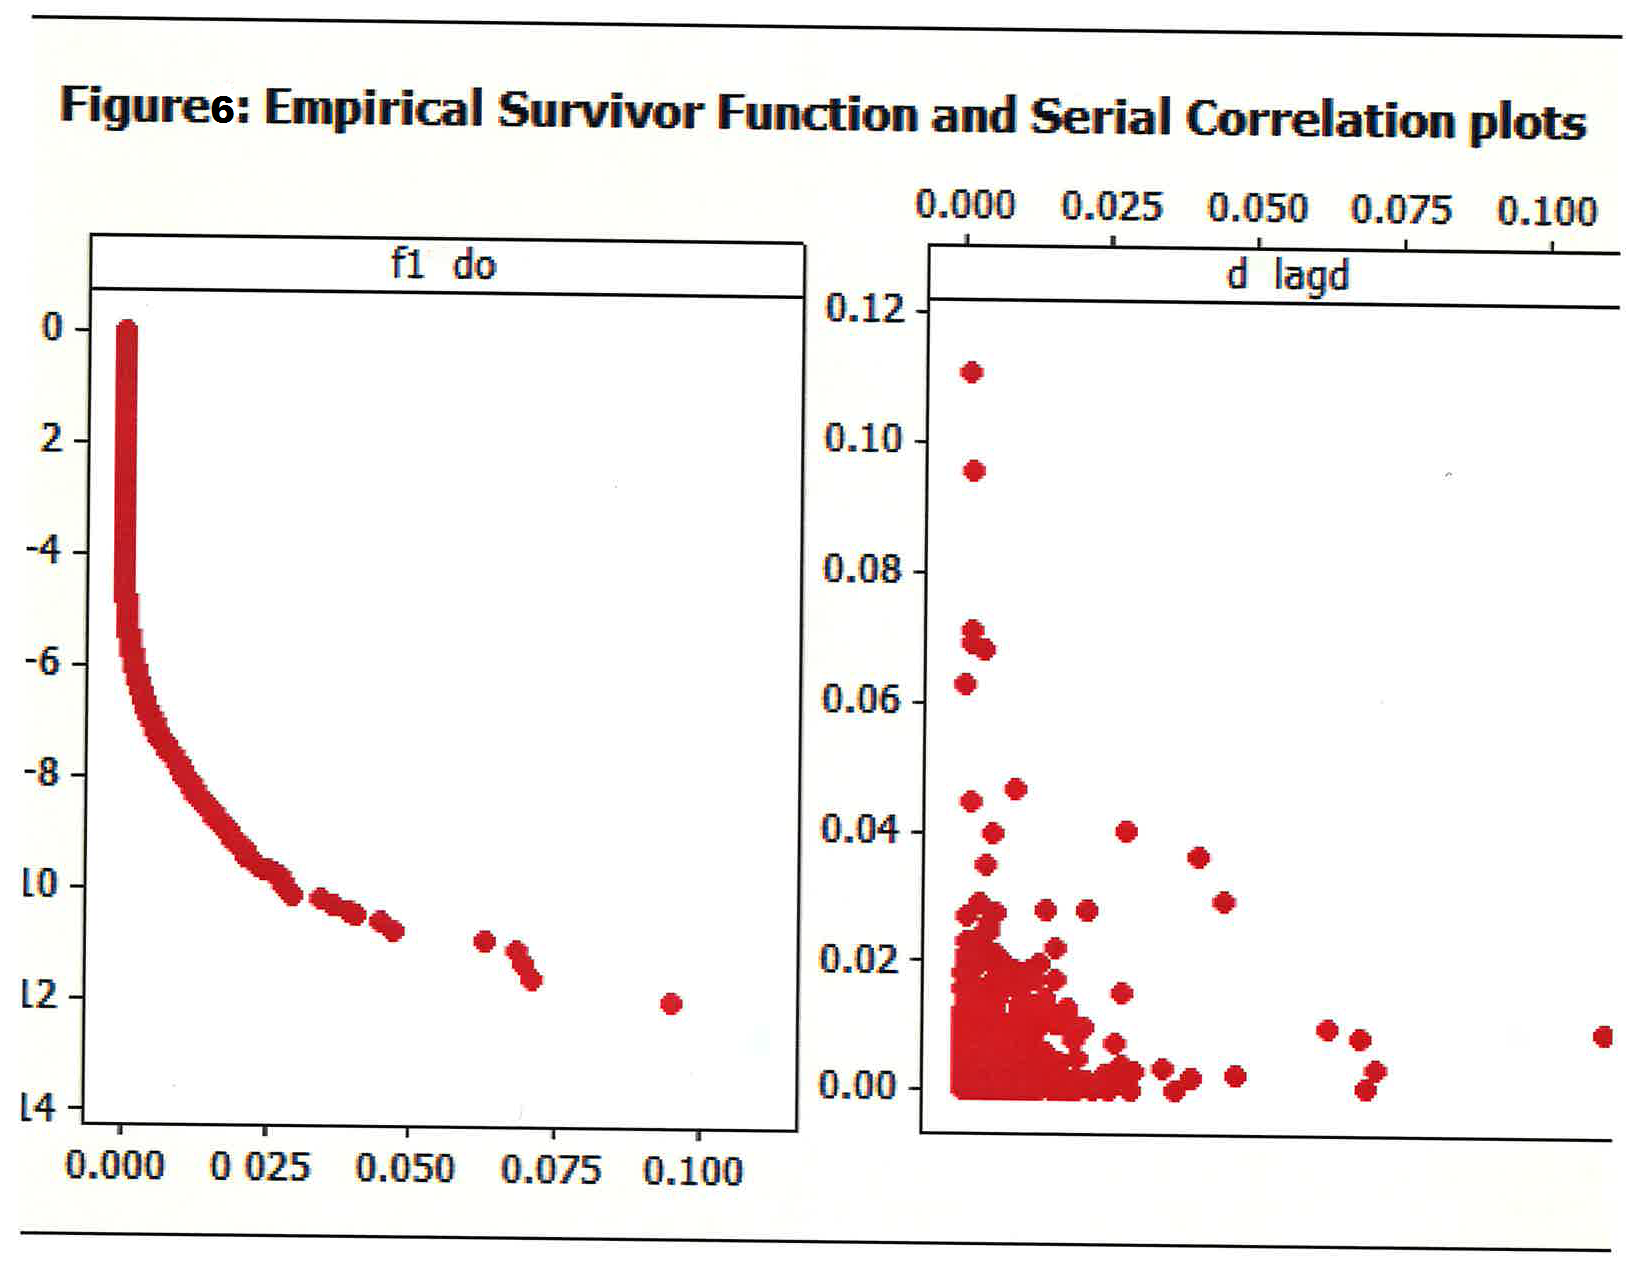
\includegraphics[width=\textwidth]{chapters/chapter_uvts/figures/Sec2-10Fig6.png}
	\caption{Empirical Survivor Function and Serial Correlation plots. \label{fig:survivor}}
	\end{figure}
	
	\begin{figure}[!ht]
	\centering
	 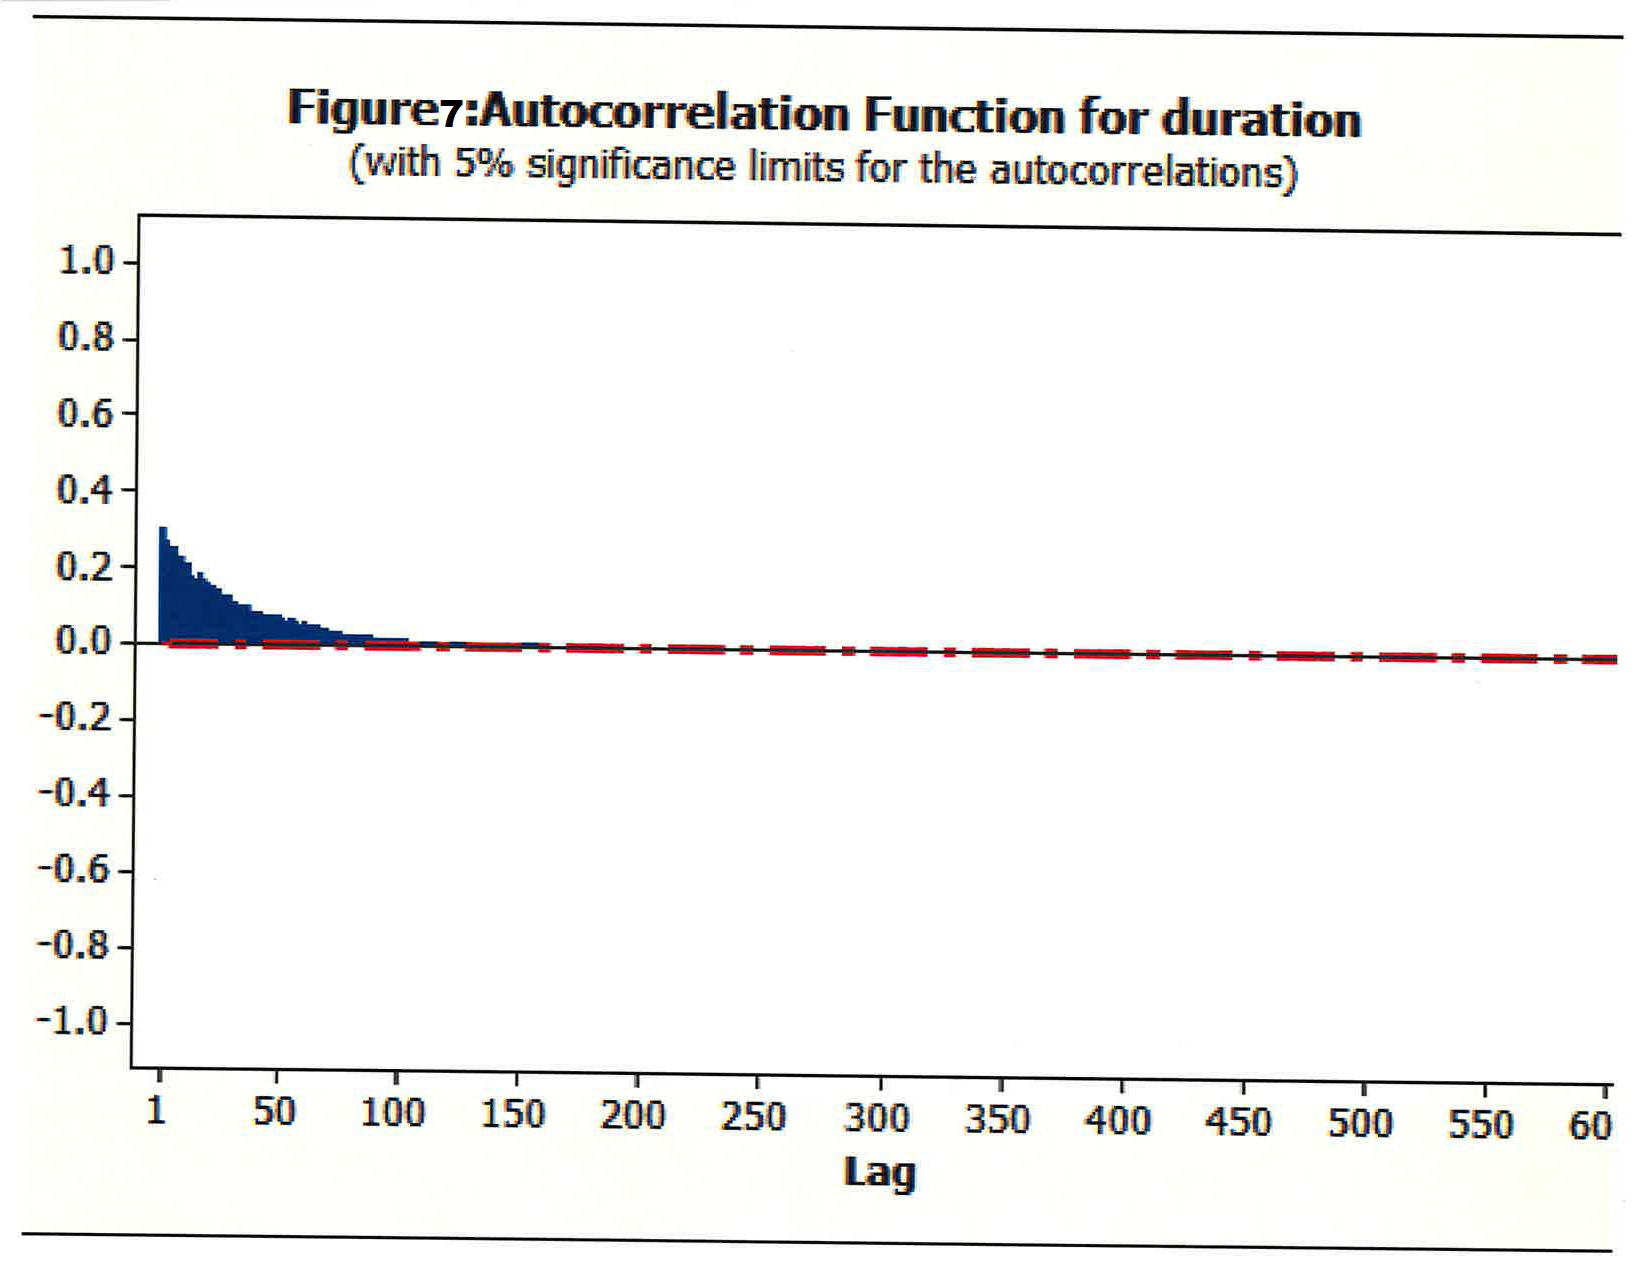
\includegraphics[width=\textwidth]{chapters/chapter_uvts/figures/Sec2-10Fig7.png}
	\caption{Autocorrelation Function for duration. \label{fig:duration}}
	\end{figure}
 
 The baseline distribution for the durations is exponential resulting from Poisson arrivals for a specified interval that assume a constant rate. It is suggested to plot log(1-$\frac{i}{n_0+1})$ against $d_{(i)}$ where $d_{(i)}$ results from the ordered durations, $d_{(1)} \leq d_{(2)} \leq ... \leq d_{(n_0)}$ calculated between successive $n_0+1$ occurrences. Departures from linearity would indicate that the exponential distribution may not hold. In addition it is also suggested to plot $d_{i+1}$ against $d_i$ to check on the dependance of durations. Cox and Lewis (1966, p14)~\cite{cox1966} state that, ``It is not clear how correlation in such data should be measured and tested; in particular it is not obvious that the ordinary correlation coefficient will be the most suitable measure with such data''. Engle and Russell (1998)~\cite{engle1998} show how the dependence in the duration data can be explicitly modeled in the context of high frequency transaction data. We illustrate this with the trading data for Microsoft (MSFT) for the month of January in the year 2013. This graph (Figure~\ref{fig:survivor}) clearly indicates that the durations do not follow an exponential distribution and do exhibit some dependence. This is confirmed by the autocorrelation function for durations (Figure~\ref{fig:duration}).


Cox and Lewis (1966)~\cite{cox1966} also observe a few issues that can arise with the point-process type data. It is possible that two or more events recorded as happening at the same time. This may be due to latency issues but if they occur due to genuine coincidences it is better to analyze the number of events attached to each occurrence time as a variate separately. Further complications are that there may be events, such as price and volume that may be interdependent and events that occur with related series that may be useful for modeling and predicting the future occurrence times.


\subsection{Stylized Models for High Frequency Financial Data}


There has been a great deal of interest in studying market micro-structure to better understand the trading mechanisms and the process of price formation. With the availability of Trades and Quotes (TAQ) data that contains all equity transactions on major exchanges, it has now became possible to better understand the market micro-structure. The extensive details from the order books over multiple exchanges have provided massive amount of data. Analyzing these data will be taken up in later chapters as well. Here we want to present some unique characteristics of the high frequency data and present most commonly used models in practice. To reiterate, the transactions (trades, quotes, bids, etc) may occur at any point in time (Figure~\ref{fig:exchhours}) during the exchange hours as given below.
	\begin{figure}[!ht]
	\centering
	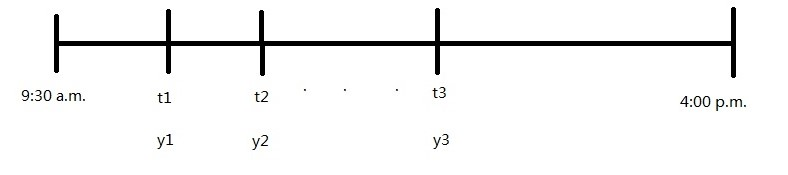
\includegraphics[width=\textwidth]{chapters/chapter_uvts/figures/33d1.jpg}
	\caption{Exchange hours. \label{fig:exchhours}}
	\end{figure}
High-frequency data refer to the `tick' `$t_i$' data which contains, in addition to the exact time of even occurrence, `$y_i$' called marks that may refer to all other elements of the limit order book such as traded price or quote etc. The traditional time series methods that we discussed in the context of low frequency data analysis are not applicable here as the ticks can occur at any point in time when the exchange are open. Standard econometric techniques are for data in discrete time intervals. Aggregating the high-frequency data to some fixed time interval will not capture the advantages of having access to detailed transaction data. Even for some heavily traded stocks, if the intervals are chosen to be short, there may be many intervals with no data and if the intervals are long, the microstructure features will be lost. Also certain key features such as the imbalance between bid side and ask side of the limit order book and when and how the market orders cross the spread are not easy to aggregate in a fixed time interval, however short or long it may be. Moreover, the timings of transactions provide valuable information for trading. Some noted features of high frequency data are:

\begin{itemize}
\item \textbf{Nonsynchronicity:} Different stocks have different trade intensities and even for a single stock, the intensity can vary over a day. For the aggregated low frequency (daily) data, thus, we cannot assume that daily returns occur in equally-spaced time series.

\item \textbf{Multiple transactions with the same time stamp:} It is possible that in periods of heavy trading especially in the opening and closing times of the exchange, each tick may contains multiple transactions. For the analysis of this type of occurrence, simple aggregate summary measures to more elaborate measures such as the variation in prices in addition to average prices are suggested.

\item \textbf{Multiple Exchanges:} In the US market there are at least sixteen known lit exchanges; due to latency issues there could be time delays in recording the submission times of orders that get dispatched at the same time. Also with the rule (NBBO) on getting best price anywhere in the market, an aggregated view of the market given a fixed time interval can miss capturing the dependency over exchanges. 

\item \textbf{Intra-day Periodicity:} Generally, it is observed for stocks transaction activities are higher near the open and the close than in the middle of the data. Thus volatility is higher, immediately after the opening and before the closing of the market resulting in U-shape pattern.

\item \textbf{Temporal Dependence:} High frequency data generally exhibit some dependence. The dependence is due to
    \begin{itemize}
    \item price discoveries
    \item bid-ask bounce
    \item Execution clustering of orders
    \end{itemize}
Under aggregation with low frequency data generally the dependence tends to decrease.

	\begin{figure}[!ht]
	\centering
	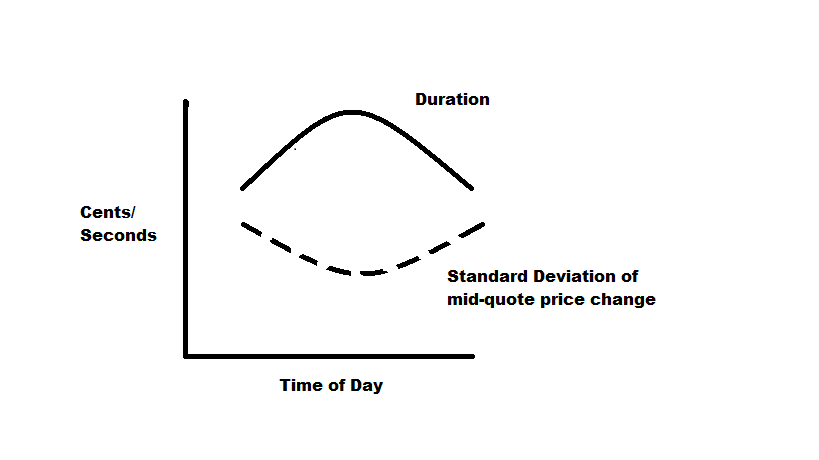
\includegraphics[width=\textwidth]{chapters/chapter_uvts/figures/Sec2-10Fig8.png}	
	\caption{Typical Diurnal patterns. \label{fig:diurnal}}
	\end{figure}

\item Volatility, volume, spread are higher near the open and close.

\item Time between trades, shorter near open and close.
\end{itemize}


\noindent\textbf{Stylized fact 6: Negative autocorrelation in returns:} Non-synchronous trading and bid-ask bounce both can introduce negative lag-1 autocorrelation in the returns. See Roll (1984)~\cite{????} and Lo and Mackinlay (1990)~\cite{lo1990}.


We want to briefly discuss the Roll model; on a typical day of trading stocks exhibit price changes numerous times. These changes signify merely the market friction, the friction between the demand and supply side and they are not necessarily due to true information about the stock. Assume that the true price (unobservable) follows a random walk model (\ref{eqn:?????}) as, 
	\begin{equation}\label{eqn:2plowstar}
	p_t^*=p_{t-1}^* + \epsilon_t 
	\end{equation}
and the observed price,
	\begin{equation}\label{eqn:2lowpstar}
	p_t = p_t^* + u_t
	\end{equation}
with `$\epsilon_t$' denoting the true information about the stock and `$u_t$' denoting the market friction. But the observed return,
	\begin{equation}\label{eqn:2firstrtlow}
	r_t=p_t-p_{t-1} = \epsilon_t + u_t - u_{t-1}
	\end{equation}
inducing the negative autocorrelation of lag 1 in the return due to the carry over term, `$u_{t-1}$'. The term on the right-hand side because of zero autocorrelation beyond lag-1 can be written as MA(1) model:
	\begin{equation}\label{eqn:2lowrt}
	r_t=a_t - \theta a_{t-1}
	\end{equation}
The value of `$\theta$' generally tends to be small, but nevertheless significant. 


\noindent \textit{Commonly used duration models:} The timing aspect of transaction was discussed in Easley and O'Hara (1992)~\cite{easley1992} and a rigorous set of tools was developed by Engle and Russell (1998)~\cite{engle1998}, as an alternative to fixed interval analysis. Treating the ticks as random variables that follow a point process, the intensity of transactions in an interval of length, $\Delta$, is defined as
	\begin{equation}\label{eqn:2lambda}
	\lambda(t) = \lim\limits_{\Delta \rightarrow 0}\frac{E[N(t+\Delta) - N(t)|F_t]}{\Delta}
	\end{equation}
where $N(t)$ denotes the number of ticks until `t' and $F_t$ is the information available until that time. The commonly used model for such arrival rates is Poisson that implies that the time between the two successive ticks is independent of pairwise ticks and follows an exponential distribution. But the duration data, $d_i = t_i - t_{i-1}$ exhibit some dependence, thus implying that time moves faster sometimes, faster than the clock time. The intensity rate, $\lambda(t)$ is not a constant, which is a typical characteristic of the exponential distribution. We briefly outline how the durations are modeled. For detailed discussion, see Tsay (2010)~\cite{tsay} or Lai and Xing (2008, Section 11.2)~\cite{lai1}. The autoregressive conditional duration (ACD) model is defined as follows:
	\begin{equation}\label{eqn:2dipsi}
	\begin{split}
	d_i&= t_i - t_{i-1} = \psi_i\varepsilon_i, \text{ and} \\
	\psi_i&= \alpha + \sum_{j=1}^p\alpha_j d_{t-j} + \sum_{v=1}^q\beta_v\psi_{i-v}
	\end{split}
	\end{equation}
where $\varepsilon_i$ are i.i.d. with $E(\varepsilon_i) = 1$; If $\varepsilon_t's$ are assumed to follow exponential the models (\ref{eqn:}) is called E(xpotential)ACD. Two alternative models WACD and GGACD are based on the following specification for the errors:
	\[
	\begin{split}
	\text{Weibull: }h(x) &= \frac{\alpha}{\beta^{\alpha}}x^{\alpha-1}\exp\left\{-(\frac{x}{\beta})^{\alpha}\right\} \\
	\text{Generalized Gamma: } y &= \lambda\frac{x}{\beta}
	\end{split}
	\]
where $\lambda = \frac{\sqrt{K}}{\sqrt{K+\frac{1}{\alpha}}}$. The hazard function of Generalized Gamma is quite flexible and may fit better various patterns. The stationary conditions would require that the roots of $\alpha(B) = 1 - \sum_{j=1}^q(\alpha_j+\beta_j)B^j$ are outside the unit circle when $g= \max(p,q)$ and $B$ is the back-shift operator. It is clear that the model (\ref{eqn:2dipsi}) is similar to GARCH$(p, q)$ model given in (\ref{eqn:}). The estimation is typically done through conditional maximum likelihood and all inferences are asymptotic.


An alternative more direct ARMA type model for log durations is suggested by Ghysels, Gourieroux and Jasiak (2004)~\cite{jasiak}:
\begin{equation}\label{eqn:21lnd}
	\ln{(d_i)} = \omega + \sum_{j=1}^p\alpha_j\ln{(d_{t-j})} + \sum_{j=1}^v\beta_j\varepsilon_{i-j} + \varepsilon_i
	\end{equation}
and $\varepsilon_i = \sqrt{h_i^v}u_i, h_i^v = \omega^v + \sum_{j=1}^{p^v}\alpha_j^v\varepsilon_{i-j}^2 + \sum_{j=1}^{q^v}\beta_j^vh_{i-j}^v$ where $u_i \sim N(0,1)$ i.i.d.; here the conditional mean and variance of durations are assumed to be separable. The duration volatility that is modeled using the second equation in (\ref{eqn:}) is interpreted as `liquidity' risk. \\


\noindent \textbf{Other Duration Related Models:} So far the discussion has been around modeling the durations, but the information set, $F_t$ has information on `marks', the information associated with the past ticks, such as the number of units transacted, price etc. McCulloch and Tsay (2009)~\cite{} suggest the following model:
	\begin{equation}\label{eqn:2lndi}
	\ln{d_i} = \beta_0 + \beta_1\ln{(d_{t-1})} + \beta_2s_{i-1} + \sigma\varepsilon_i
	\end{equation}
where $s_i$ is the size of the $i$th price change measured in ticks; other relevant variables can be easily added to this model.


\subsection{Models for Multiple Assets: High-Frequency Context}


There is a considerable interest in extending the univariate duration models to multiple stocks or to multiple types of arrival processes. Because investment managers generally consider a portfolio of stocks rather than a single one, it is important for them to follow the transaction processes of several stocks simultaneously. Because of non-synchronous trading relating two stocks with different trading intensities on a common time scale is somewhat difficult. Engle and Lunde (2003)~\cite{englelunde} establish the following model for a bivariate point process for trades and quotes:
	\begin{figure}[!ht]
	\centering
	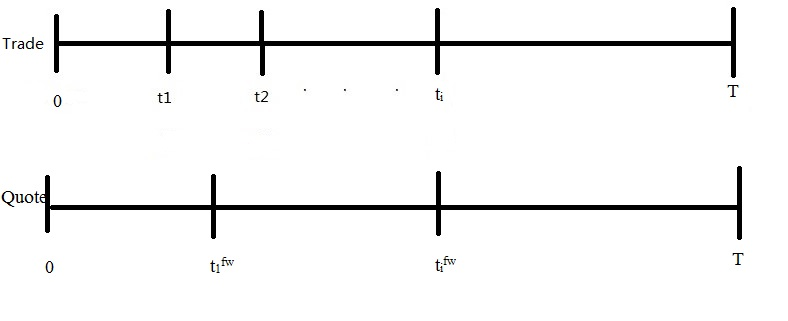
\includegraphics[width=\textwidth]{chapters/chapter_uvts/figures/33d3.jpg}
	\caption{Trades and Quotes. \label{fig:tradeactdoubline}}
	\end{figure}
Define $x_i = t_i - t_{i-1}$ as trade duration and $y_i = t_i^{f_w} - t_{i-1}^{f_w}$ as the forward quote duration; our goal is to model $(x_i,y_i)$ as a bivariate duration process but the underlying timings are not synchronized. Thus define, if $y_i > x_i$, then
	\begin{equation}\label{eqn:anothertildey}
	\widetilde{y}_i = (1 - d_i)y_i + d_ix_i
	\end{equation}
where $d_i$ is indicator variable, $d_i = I_{\{y_i>x_i\}}$. Model ($x_i,\widetilde{y}_i$) as censored process. The equation (98) provides a mechanism in a way to align the two processes. The joint distribution is given by
	\begin{equation}\label{eqn:2pxiyi}
	p(x_i,\widetilde{y}_i | F_{i-1},\omega) = g(x_i|F_{i-1},\omega_1) f(\widetilde{y}_i | x_i,F_{i-1},\omega_2)
	\end{equation}
The first term is the trade density and the second term is the quote density. The $\psi_i$ terms as in (\ref{eqn:}) are modeled as EACD, $\psi_i= f(\psi_{i-1},x_{i-1},z_{i-1})$ and quote density is also modeled as EACD after adjusting for censoring:
	\begin{equation}\label{eqn:2fdot}
	f(y_i|\cdot) = [h(y_i|\cdot)]^{1-d_i} \times S(x_i|\cdot)^{d_i}
	\end{equation}
The estimation of the parameters are done through quasi maximum likelihood. Using data for eight stocks, Engle and Lund (2003)~\cite{englelunde} observe that high trade arrival rates, large volume per trade, wide bid-ask spreads, all predict more rapid price revisions. The model given in Engle and Lund (2003)~\cite{englelunde} can be conceptually applied to any two point processes. Extending this concept to more than two processes could be of interest to the traders who may want to monitor the trading exchanges simultaneously. 


\section{Time Aggregation and Loss of Information}


\section{Realized Volatility and Econometric Models}


Estimating the volatility using the high-frequency data has received a great deal of attention lately. In the low frequency (daily) level some estimators based on select prices were presented. Intra-day dynamics of volatility is of interest to traders and that is not fully captured by the stock price indicators sampled during the day. If higher frequency data are used to estimate volatility of lower frequency data, it is important to know the model for the return at the lower frequency. To illustrate this, we consider data observed at two time scales; although they are at low frequency level, the concept can be easily extended to high-frequency context. If $r_{t,i}$ is the $i$th day return in $t$th month, the $t$th month return assuming there `n' trading days, $r_t^m = \sum_{i=1}^nr_{t,i}$. Note that $\sigma_m^2 = \Var(r_t^m|F_{t-1}) = \sum_{i=1}^n \Var(r_{t,i} | F_{t-1}) + 2 \sum_{i<j} \Cov(r_{t-i},r_{t-j} | F_{t-1})$. If $r_{t,i}$ is white noise sequence, then
	\begin{equation}\label{Eqn:2hatsigmasq}
	\hat{\sigma}_m^2 = \frac{n}{n-1} \sum_{i=1}^n(r_{t,i} - \overline{r}_t)^2
	\end{equation}
But we had observed that in the high frequency data returns do exhibit some serial correlation and so adjusting (\ref{eqn:}) for serial correlation is important to get a more accurate estimate of volatility. A simpler estimate of $\sigma_m^2$ is the so called realized volatility ($RV_t$)
	\begin{equation}\label{eqn:2RV}
	\text{RV}_t = \sum_{i=1}^n r_{t,i}^2
	\end{equation}
But in the estimation of intra-day volatility, the number of sampling intervals, `$n$' and hence, `$\Delta$', the interval size can affect the estimate. If $\Delta \rightarrow 0$, the value $RV_t$ in the $\Delta$-interval goes to infinity. Thus the optimal choice of `$\Delta$' is crucial and is reviewed below, for a judicious choice.


Bandi and Russell (2006)~\cite{bandi} argue that the observed price is the sum of efficient price and a friction price (see (\ref{eqn:})) that is induced by bid-ask bounce, price discreteness etc. Thus the observed variance such as (\ref{eqn:}) is the sum of variance of the efficient returns and the variance of micro-structure noise. As they indicate, both are useful: ``The variance of the efficient return process is a crucial ingredient in the practice and theory of asset valuation and risk management. The variance of microstructure noise components reflects the market structure and the price setting behavior of market participants and thereby contains information about the market fine-grain dynamics.'' Both components can be estimated using high frequency data but sampled at different frequencies. Data sampled at low frequency are used to estimate the efficient return variable and the data of high frequency are used to estimate the microstructure noise variance.


On any given day, assume that the observed price, at time `$i$' is as in (\ref{eqn:})
	\begin{equation}\label{eqn:2pi2}
	p_i = p_i^* + u_i, \quad i= 1,2,\ldots,n
	\end{equation}
where $p_i^*$ is the efficient price and $u_i$ is the of microstructure noise. Dividing a trading day into $M$ sub-periods, where $\delta= 1/M$ is the size of the sub-period, write the observed returns as
	\begin{equation}\label{eqn:2rji2}
	r_{j,i} = r_{j,i}^* + \varepsilon_{j,i}, \quad j= 1,2,\ldots,M
	\end{equation}
Assume that the frictions, $u$'s are i.i.d. mean zero and variance $\sigma_{u}^2$. Because $\varepsilon_{j,i}= u_{(i-1)+j\delta} - u{(i-1) + (j-1)\delta}$, $\Var(\varepsilon_{j,i})= 2\sigma_{\eta}^2$. It has been noted already that the return series exhibit negative first order autocovariance and $\varepsilon$'s can be taken as MA(1) structure for the $\eta$'s. Thus, the returns are computed at higher frequency at which the new information arrives. Thus $\sum_{j=1}^M r_{j,i}^2/M$ can be used to estimate noise variance. For the estimation of efficient price variance, we need to consider an  optimal division of a day into `M' number of subperiods. The optimal sampling frequency over `$n$' day is chosen as $\delta^* = 1/M^*$ with $M^*= \left[\dfrac{\hat{Q}}{\hat{\alpha}}\right]^{\frac{1}{3}}$, where $\hat{\alpha} = \sum_{i=1}^n\sum_{j=1}^M\overline{r}_{j,i}^2/(nM)$ and $\hat{Q}_i = \frac{M}{3}\sum_{j=1}^M\hat{r}_{j,i}^4$. Based on the analysis of a sample of S\&P 100 stocks mid quotes for the months of February 2002, Bandi and Russell (2006)~\cite{bandi} conclude that 5-min frequency is optimal and the 15-min interval may provide the variance estimates `excessively volatile'. The economic benefit of optimal sampling is that high frequency traders can employ a realistic variance forecasts in formulating the entry and exit strategies. Additional references on this topic include, A{\"\i}t-Sahalia, Mykland and Zhang (2005)~\cite{ait2005often} and Barndoff-Nielsen and Shepard (2002)~\cite{barndorff2002econometric}.


\section{Analytics from Machine Learning Literature}


The technical trading rules that are discussed in Chapter 3 involve a relatively small information set to carry out prediction. It treats each of the $n$ time series of asset returns as autonomous. As pointed out by Malkiel (2012)~\cite{malkiel}, these rules can be easily implemented by most market participants if such opportunities should emerge, and market efficiency would rule them out as winning strategies. More powerful prediction methods using a very large set of potential predictors and yet capable of avoiding overfitting are needed to take advantage of transient opportunities. We give a overview here of recent advances in high-dimensional regression and classification and in machine learning and computer science to handle different types of data (including text mining).


\section{Other Topics: Bet Size etc.}













\section{Exercises (starred items have $R$-codes available)}


\begin{enumerate}[1.]
\item Consider the exchange rate daily data from December 4, 2006 to November 5, 2010 (Rupee versus Dollar, Pound and Euro), Rates.csv.
\begin{enumerate}[(a)]
\item Compute the sample average, standard deviation and the first order autocorrelation of daily returns over the entire sample period.  Test if the mean and the first order autocorrelation are significantly different from zero using the tests proposed in Section 2.3.2. 

\item Plot histograms of the returns over the entire sample period; Does the distribution look normal?  Test it through Jarque-Bera test in (\ref{eqn:?????}).

\item Aggregate the data at the weekly level; do (a) and (b) on the aggregated data. Compare the result with the result for the daily level.
\end{enumerate}

\item For the returns of all three time series in problem 1,  construct
\begin{enumerate}[(a)]
\item ARMA models for the returns; identify the model structure via ACF and PACF.

\item  GARCH models for the squared returns; compare the model coefficients for the three series.  Comment on the difference if any.

\item Is there a co-movement among the three exchange-rate series? To make the plots on a comparable scale, convert the starting points of the series unity. Does the co-movement vary over different time regimes? (Back up your claim with solid analysis.) Identify the transition states and speculate how you can exploit this for trading decisions. 
\end{enumerate}

\item Exchange Rates: The file \texttt{Exchange Rates.csv} contains exchange rates between US dollar and twenty-five major currencies. The daily data spans from Jan 3, 2000 to April 10, 2012. Use this data to perform the following tasks: after computing the returns, $r_t=\log(p_t)-\log(p_{t-1})$ for each series.

\begin{enumerate}[(a)]
\item Plot histograms of the returns and test if the distributions are normal, via Q--Q plots.

\item Compute the auto-correlation function and identify which lags are significant. What is the tentative ARMA model?

\item Is there any ARCH effect? Why?

\item Fit GARCH(1,1,) and IGARCH(1,1) models using both normal and t-distributions for the innovations. Which volatility model appears to be the best?
\end{enumerate}

 \item Exchange rates: Consider the original series, $p_t$, for the duration starting June 11, 2003.
 Answer the following after dividing each series by $p_1$, so that the starting points are the same.
\begin{enumerate}[(a)]
\item Identify for each series, if there are any regime changes. Test if these changes are statistically significant.

\item Identify how many clusters are there and if the membership changes under different regimes.

\item Are the series co-integrated? Use Johansen's rank test (\ref{eqn:}) to identify the number of co-integrating relationships. Interpret the coefficients of the co-integrating vectors.

\item Compare the results in (c)  with (b). What is the connection between clustering and co-integration? Briefly discuss.
\end{enumerate}


\item Consider daily price of Apple stock from Apple.cav. The data can be obtained from Yahoo Finance and have 7 columns (namely, Date, Open, High, Low, Close, Volume, Adj Close). We focus on the adjusted closing price in the last column. Note the data needs to be reversed from the past to the recent. 
\begin{enumerate}[(a)]
\item Compute the daily log returns. Is there any serial correlation in the daily log returns? Use the test for white noise as outlined in the text. 

\item Consider the pivot quantities on the average of high and low price and the average of high, low and close prices. Compute the returns based on the pivot log prices and test for serial correlation. Compare this result with the finding in (a). 

\item Consider the log price series of AAPL stock. Is the log price series unit-root nonstationary? Perform a unit-root (Dickey-Fuller) test to answer the question and present your conclusion.
\end{enumerate}

\item Consider daily price of Apple stock again.
\begin{enumerate}[(a)]
\item Compute various measures of variance computed from the entries of the price bars. Comment on their correlation with log volume. 

\item Use the ARIMA modeling to come up with a parsimonions model for log volume. Comment on the model accuracy by setting aside a validation data set. 
\end{enumerate}


\item The \textit{Roll} model for trade prices discussed in the text can be more specifically stated as,
	\[
	\begin{split}
	p_t^*&= p_{t-1} + \epsilon_t, \;\;\;\;\; \epsilon_t \sim N(0,\sigma^2) \\
	\text{and } p_t&= p_t^* + c s_t, \;\;\;\;\; \text{where }s_t \in \{+1,-1\}
	\end{split}
	\]
Here $p_t^*$ is the ``true'' value of a security and $p_t$ is the observed trade price, which differ because of the bid-offer spread: $c$ is the half-spread and $s_t$ is the direction of the $t$th trade. $s_t$ and $\epsilon$ are serially independent and independent of each other.
\begin{enumerate}[(a)]
\item Calculate the serial correlation of the observed prices $p_t$. Construct an MA(1) model with the same autocorrelation structure. Of the two such models, take the invertible one. 

\item For the invertible model, construct the associated AR model. 

\item Use the model to show how to estimate the bid-ask spread and apply the results on the Apple data used in Problem (5) and (6). \\
\end{enumerate}


\textbf{Questions 8--10 refer to Level III data descried below:} \\


The dataset consists of (CSV) file that contains the entire trading session, including early and late hours from 6:00~a.m. to 8:00~p.m. EST. It contains intraday depth book activity several major tickers from up to 5 major national exchanges: Nasdaq, Direct Edge, NYSE, ARCA, and BATS (exact number of exchanges depends on the historical period). All messages are consolidates into one file ordered by timestamp. This dataset allows to build a full national depth book (super book) at any moment intraday. 

\begin{table}[h!]
   \caption{Column Format}
   \centering
   \begin{tabular}{p{2cm}p{8cm}} 
   \textbf{Column} & \text{Description} \\ \hline
   Timestamp & Number of milliseconds after the midnight. \\ \hline
   Ticker & Equity symbol (up to 8 characters) \\ \hline
   Order & Unique order ID. \\ \hline
   T & Message type. Allowed Values: \newline
	~~\llap{\textbullet}~~ ``B''--Add buy order \newline
	~~\llap{\textbullet}~~ ``S''--Add sell order \newline
	~~\llap{\textbullet}~~ ``E''--Execute outstanding order in part \newline
	~~\llap{\textbullet}~~ ``F''--Execute outstanding order in full \newline
	~~\llap{\textbullet}~~ ``D''--Delete outstanding order in full \newline 
	~~\llap{\textbullet}~~ ``X''--Bulk volume for the cross event \newline
	~~\llap{\textbullet}~~ ``T''--Execute non-displayed order  \\ \hline
   Shares & Order quantity, available for the ``B'', ``S'', ``E'', ``X'', ``C'', ``T'' messages. Zero for ``F'' and ``D'' messages. \\ \hline
   Price & Order price, available for the ``B'', ``S'', ``X'', and ``T'' order messages. Zero for cancellation and executions. The last 4 digits are decimal digits. The decimal portion is padded on the right with zeros. The decimal point is implied by position; it does not appear inside the price field. Divide by 10000 to convert into currency value. \\ \hline
   MPID & Market Participant ID associated with the transaction (4 characters) \\ \hline
   MCID &U Market Center Code (originating exchange--1 character)
   \end{tabular}
\end{table}


For the analysis of Problems 8--10, we consider the data for CISCO.

 
\item You need to aggregate the data into 5-min intervals before answering the following.
\begin{enumerate}[(a)]
\item Let $x_t$ denote the number of trades in the $t$th 5-minute interval. Ignore the time gaps between trading days. Plot the time series and its ACF. Determine if there are intraday period patterns in the series.

\item Using the last transaction in the $t$th 5-minute interval as the stock price in that interval, plot the
time series $y_t$ of 5-minute returns during the period and the corresponding ACF.

\item Consider the bivariate time series ($x_t$, $y_t$). How does $y_t$ vary with $x_t$? Are there intraday periodic patterns in ($x_t$, $y_t$)?

\item Plot the durations of the transaction times for Mondays and Fridays. Is there any difference in the
patterns?

\item Fit GARCH models for the durations and interpret the coefficients.

\item Is there any particular exchange that offers better price?
\end{enumerate}



\item Use the transaction data in Problem 8. There are seventy-eight five-minute intervals in a trading day. Let $d_i$ be the average of all log durations for the $i$th 5-minute interval across all trading days. Let $t_j$ be tick time of a trade during the $i$th 5-minute interval, define an adjusted duration as $\Delta t_j^* = \Delta t_j/\exp(d_i)$ where $\Delta t_j = t_j - t_{j-1}$.
\begin{enumerate}[(a)]
\item Is there a diurnal pattern in the adjusted duration series?

\item Build EACD and WACD models for the adjusted duration and compare them. Now aggregate the data over the 5-minute intervals; Let $r_t$ be the return and $V_t$ is the volume of transactions in the $t$th interval.

\item Is there any relationship between the volume $V_t$ and volatility $r_t^2$ . If there is develop a model that will capture the dependence of volatility on volume. Let $\overline{p}_t$ be the average price in the $t$th 5-minute
interval.
\end{enumerate}


\item Use the CISCO execution data only; aggregate at various time intervals: 1~min, 2~min, \dots, 15~min. For these levels record
\begin{enumerate}[(a)]
\item Average price, VWAP, realized volatility and aggregate volume.

\item By relating the returns and volatility estimates based on average price to realized volatility, identify the optimal duration for aggregation that will cancel out the market friction but pick up the true information. (You may want to refer to Bandi and Russell (2006)~\cite{bandi}). 
\end{enumerate}




\end{enumerate}



